\documentclass[sigconf]{acmart}
%\documentclass[format=acmsmall, review=false, screen=true]{acmart}
 \usepackage{booktabs} 

% \usepackage{epstopdf}
% \usepackage{textcomp} % copyright symbol
% \usepackage{adjustbox} % scaling figure size
% \usepackage{textcase}
% \usepackage{amsfonts}
\usepackage{graphicx}


% \usepackage{enumerate}
% \RequirePackage{xspace}
% \RequirePackage{graphics}
 \usepackage{xcolor}
% \RequirePackage{textcomp}
% \usepackage{mathrsfs}
% \usepackage{lipsum}
\usepackage{listings}
% \usepackage{multirow}
% \usepackage[english]{babel}
% \usepackage{array}
% \usepackage{pifont} % check mark
% \usepackage{stmaryrd}
\usepackage{footnote}
% \usepackage{makecell}
% \usepackage{xparse}
\usepackage{algorithm}
% \usepackage{algpseudocode}
\usepackage{amssymb}
\usepackage{stmaryrd}
\usepackage{amsmath}
%\usepackage{upgreek}
%\usepackage{mathtools}
% \usepackage{amsfonts}
% \RequirePackage{xspace}
% \RequirePackage{graphics}
% \usepackage{xcolor}
% \RequirePackage{textcomp}
% \usepackage{keyval}

\usepackage{xspace}
% \usepackage{mathrsfs}
\usepackage{paralist}
% \usepackage{lipsum}
% \usepackage{listings}
\usepackage{multirow}
% \usepackage{array}
\usepackage{adjustbox} % scaling figure size
% \usepackage{textcase}
% \usepackage{makecell}
\usepackage[inline]{enumitem} % errors
\usepackage{makecell}
% \usepackage{flushend} % equalize reference columns
%\usepackage{tabularx}
% \usepackage{standalone}
% \newif\ifbuildtikz
% \newcommand{\addtikz}[2]{\ifbuildtikz{\input{#1}}\else{\includegraphics[scale=#2]{#1}}\fi}
%
% activate rebuild of pictures by default;
% replace 'true' by 'false' to just include the graphics from the sub-pdfs
% this should increase build-time drastically, but at the cost that changes to the tikz-code are not considered
% \buildtikztrue
%\usepackage{etoolbox}
%\usepackage{IEEEtrantools} %equation

\RequirePackage{tikz}
 \usetikzlibrary{arrows,automata,shapes,calc,through,decorations.pathmorphing,decorations.fractals,chains,shapes.multipart}

%\usepackage{standalone}
%\newif\ifbuildtikz
%\newcommand{\addtikz}[2]{\ifbuildtikz{\scalebox{#2}{\input{#1}}}\else{\includegraphics[scale=#2]{#1}}\fi}
%
% activate rebuild of pictures by default;
% replace 'true' by 'false' to just include the graphics from the sub-pdfs
% this should increase build-time drastically, but at the cost that changes to the tikz-code are not considered

%\usepackage{beramono}
 \definecolor{javared}{rgb}{0.6,0,0} % for strings
 \definecolor{javagreen}{rgb}{0.25,0.5,0.35} % comments
 \definecolor{javapurple}{rgb}{0.5,0,0.35} % keywords
 \definecolor{javadocblue}{rgb}{0.25,0.35,0.75} % javadoc


 \lstset{
 	language=Python,
 	morekeywords={function,for, end, input, output, parameters, each,in,with,is,valid,from,to,property,stop,variable,counterexample,forall,then, begin, algorithm, Initialization, Require, Initialize, increase, length, find,getModelByName,strrep,copyModel,addState,addParam,replace,addTransition,getCopyState,getCopyState,addTransition,formode,fortran,sfroot,getTransitions,getStates,notDefaultTransition}, % note otherkeywords vs. morekeywords
 	%deletekeywords={invariants,invisible,inside,index},
 	basicstyle=\ttfamily\small,
 	keywordstyle=\color{javapurple}\bfseries,
 	stringstyle=\color{javared},
 	commentstyle=\color{javagreen}\sffamily\itshape,
 	%commentstyle=\color{javagreen},
 	morecomment=[s][\color{javadocblue}]{/**}{*/},
 	numbers=left,
 	%tabsize=1,
 	numberstyle=\color{black},
 	stepnumber=2,
 	numbersep=0pt,
 	tabsize=2,
 	showspaces=false,
 	showstringspaces=false,
 	xleftmargin=0.5em,
 	frame=single,
 	framexleftmargin=1em,
 	mathescape,
 	escapeinside={(*@}{@*)}
 }

\usepackage{subfigure}
%\usepackage{subfig}
%\usepackage{appendix}
%\usepackage[toc,page]{appendix}
\usepackage{arydshln} % hdashline
% \usepackage[free-standing-units]{siunitx}

% \usepackage{circuitikz}

%\usepackage[pdftex]{hyperref}

 \hypersetup{
 pdftitle={},
 pdfauthor={},
 pdfkeywords={},
 colorlinks=true,
 citecolor={purple},
 linkcolor={blue},
 bookmarksopen=true,
 bookmarksnumbered=true
 }

\newcommand\IL[1]{$\clubsuit$\footnote{IL: #1}}
\newcommand\JW[1]{$\spadesuit$\footnote{JW: #1}}
\newcommand\OS[1]{$\heartsuit$\footnote{OS: #1}}
\newcommand\RA[1]{$\ddagger$\footnote{RA: #1}}

% marking changes

\newcommand{\commenttaylor}[1]{{\color{red}[TTJ: #1]}}
\newcommand{\commentluan}[1]{{\color{blue}[LN: #1]}}
\newcommand{\commentnote}[2]{{\color{blue}[COMMENTCHANGE: Note: #1\\#2]}}
\newcommand{\commentchange}[1]{{\color{blue}[COMMENTCHANGE: #1]}}
%\newcommand{\commentchange}[1]{\textcolor{black}{#1}}

% for nomencl to produce page links
%\renewcommand*{\pagedeclaration}[1]{\unskip, \hyperpage{#1}}
%\renewcommand{\nomname}{List of Symbols and Functions}

\newcommand{\revision}[1]{\textcolor{blue}{#1}}

\newcommand{\authcomment}[1]{\textbf{[[#1]]}}
\newcommand{\todo}[1]{\textcolor{green}{\textbf{[TODO: [#1]]}}}
\newcommand{\note}[1]{\textcolor{blue}{\textbf{[Note: [#1]]}}}
%\newcommand{\taylor}[1]{}
%\newcommand{\todo}[1]{}

%FIXED SETS

%\newcommand{\Time}{{\sf T}}                     %time domain
\newcommand{\nnt}{{\sf T}^{\geq 0}}             %nonnegative time points
\newcommand{\post}{{\sf T}^{>0}}                %positive time points
\newcommand{\Variables}{{\sf V}}                %variables

%todo: check
\newcommand{\num}[1]{\relax\ifmmode \mathbb #1\else $\mathbb #1$\fi}
\newcommand{\nnnum}[1]{\relax\ifmmode 
  {\mathbb #1}_{\geq 0} \else ${\mathbb #1}_{\geq 0}$
  \fi}
\newcommand{\npnum}[1]{\relax\ifmmode 
  {\mathbb #1}_{\leq 0} \else ${\mathbb #1}_{\leq 0}$
  \fi}
\newcommand{\pnum}[1]{\relax\ifmmode 
  {\mathbb #1}_{> 0} \else ${\mathbb #1}_{> 0}$
  \fi}
\newcommand{\nnum}[1]{\relax\ifmmode 
  {\mathbb #1}_{< 0} \else ${\mathbb #1}_{< 0}$
  \fi}
\newcommand{\plnum}[1]{\relax\ifmmode 
  {\mathbb #1}_{+} \else ${\mathbb #1}_{+}$
  \fi}
\newcommand{\nenum}[1]{\relax\ifmmode 
  {\mathbb #1}_{-} \else ${\mathbb #1}_{-}$
  \fi}

\newcommand{\reals}{{\num R}}                    %reals
\newcommand{\booleans}{{\num B}}                    %reals
\newcommand{\nnreals}{{\nnnum R}}                    %nonnegative reals
\newcommand{\realsinfty}{{\num R} \cup \{\infty, -\infty\}}                    %nonnegative reals
\newcommand{\plreals}{{\plnum R}}                    %positive reals
\newcommand{\naturals}{{\num N}}                      %natural numbers
\newcommand{\integers}{{\num Z}}                      %integers
\newcommand{\rationals}{{\num Q}}                      %rationals
\newcommand{\nnrationals}{{\nnnum Q}}                   % nonnegative rationals
%\newcommand{\Time}{{\num T}}  

% EXECUTIONS TRACES and FRAGS
\newcommand{\extb}[1]{\relax\ifmmode {\sf ExtBeh}_{#1} \else ${\sf ExtBeh}_{#1}$\fi} 
\newcommand{\tdists}[1]{\relax\ifmmode {\sf Tdists}_{#1} \else ${\sf Tdists}_{#1}$\fi} 

\newcommand{\exec}[1]{\relax\ifmmode {\sf Execs}_{#1} \else ${\sf Exec}_{#1}$\fi} 
\newcommand{\execf}[1]{\relax\ifmmode {\sf Execs}^*_{#1} \else ${\sf Exec}^*_{#1}$\fi} 
\newcommand{\execi}[1]{\relax\ifmmode {\sf Execs}^\omega_{#1} \else ${\sf Exec}^\omega_{#1}$\fi} 

\newcommand{\ctrace}[1]{\relax\ifmmode {\sf Ctraces}_{#1} \else ${\sf Ctraces}_{#1}$\fi} 

\newcommand{\trace}[1]{\relax\ifmmode {\sf Traces}_{#1} \else ${\sf Traces}_{#1}$\fi} 
\newcommand{\tracef}[1]{\relax\ifmmode {\sf Traces}^*_{#1} \else ${\sf Traces}^*_{#1}$\fi} 
\newcommand{\tracei}[1]{\relax\ifmmode {\sf Traces}^\omega_{#1} \else ${\sf Traces}^\omega_{#1}$\fi} 

\newcommand{\frag}[1]{\relax\ifmmode {\sf Frags}_{#1} \else ${\sf Frags}_{#1}$\fi} 
\newcommand{\fragf}[1]{\relax\ifmmode {\sf Frags}^*_{#1} \else ${\sf Frags}^*_{#1}$\fi} 
\newcommand{\fragi}[1]{\relax\ifmmode {\sf Frags}^\omega_{#1} \else ${\sf Frags}^\omega_{#1}$\fi} 

\newcommand{\reach}[1]{\relax\ifmmode {\sf Reach}_{#1} \else ${\sf Reach}_{#1}$\fi} 

\newcommand{\execs}{{\exec{}}}
\newcommand{\traces}{{\trace{}}}
\newcommand{\fragss}{{\frag{}}}

\newcommand{\fexecs}{{\execf{}}}
\newcommand{\ftraces}{{\tracef{}}}
\newcommand{\ffragss}{{\fragf{}}}

\newcommand{\iexecs}{{\execi{}}}
\newcommand{\itraces}{{\tracei{}}}
\newcommand{\ifragss}{{\fragi{}}}


%\newcommand{\qed}{\hfill{\rule{2mm}{2mm}}\medskip}
%\newenvironment{proof}{\trivlist\item[]\emph{Proof}:}{\unskip\nobreak\hskip 1em plus 1fil\nobreak\qed\parfillskip=0pt\endtrivlist}
\newenvironment{noqedproof}{\pf}{}
%\newcommand{\pf}{\par\noindent{\bf Proof:}~}


%\newcounter{theorem}
\newtheorem{theoremcust}{Theorem}[theorem]
%\newtheorem{lemma}[theorem]{Lemma}
%\newtheorem{example}[theorem]{Example}
%\newtheorem{corollary}[theorem]{Corollary}
%\newtheorem{claim}[theorem]{Claim}
%\newtheorem{definition}[theorem]{Definition}
%\newtheorem{proposition}[theorem]{Proposition}
\newtheorem{invariant}[theorem]{Invariant}
\newtheorem{counterexample}[theorem]{Counterexample}
% \newtheorem{remark}[example]{Remark}
\newtheorem{assumption}[theorem]{Assumption}
 
\newenvironment{remark}
{\refstepcounter{theorem} \vspace{2ex}\par\noindent
\textbf{Remark}~\textbf{\thetheorem~}}
 
%\theoremstyle{remark}
%\newcounter{example}
% \newtheorem{example}{Example}[chapter]
% {\refstepcounter{theorem} \vspace{2ex}\par\noindent
% \textbf{Example}~\textbf{\theexampletheorem~}}{\qed}
 
 
 \def\examplenonum#1#2{
	\vspace{.15in}
	\noindent
	{\bf Example #1}{\em ~(continued)}{\bf .}
	{#2}{\qed}
	}
% 
% \renewcommand{\theequation}{\thesection.\arabic{equation}}
% \renewcommand{\thefigure}{\thesection.\arabic{figure}}
% \renewcommand{\thetable}{\thesection.\arabic{table}}
% \newcommand{\Section}[1]{\section{#1}%
%    \setcounter{equation}{0}\setcounter{figure}{0}\setcounter{table}{0}%
%    \setcounter{example}{0}}
% 
% \newenvironment{anotation}[1][Nancy]{\begin{quote}\small[[[#1]]]}{\normalsize\end{quote}}
% \newcommand{\ba}{\begin{anotation}}
% \newcommand{\ea}{\end{anotation}}
% 
% \newcommand{\bcb}{\chgbarbegin}
% \newcommand{\ecb}{\chgbarend}
% \chgbarwidth 1pt
% 
% \newcommand{\dec}{\ensuremath{{:}}}
% \newcommand{\eqdef}{\mathbin{::=}}
% \newcommand{\I}{{\ensuremath{\cap}}}



% OPERATIONS ON SETS, RELATIONS AND FUNCTIONS
\newcommand{\pow}[1]{{\bf P}(#1)} % powerset
\newcommand{\inverse}[1]{#1^{-1}}
\newcommand{\range}[1]{\ms{range{(#1)}}}
\newcommand{\domain}[1]{{\it dom}(#1)}
\newcommand{\type}[1]{\ms{type{(#1)}}}
\newcommand{\dtype}[1]{\ms{dtype{(#1)}}} % dynamic type
\newcommand{\restr}{\mathrel{\lceil}}
\newcommand{\proj}{\matrel{\lceil}}
\newcommand{\restrrange}{\mathrel{\downarrow}}
\newcommand{\point}[1]{\wp(#1)}     		%point trajectory



% HYBRID AUTOMATA
\def\A{{\cal A}} % HA
\def\B{{\cal B}} % HA
\def\C{{\cal C}} % HA
\def\D{{\cal D}} % set of discrete steps
\def\E{{\cal E}} % HA
\def\F{{\cal F}} % HA
\def\G{{\cal G}} % pieces of SHIOA
\def\H{{\mathcal H}} % HA
\def\I{{\mathcal I}} % environment sequence
\def\K{{\cal K}} % environment sequence
\def\L{{\cal L}} % 
\def\M{{\cal M}} % Mode switching transitions
\def\O{{\mathcal O}} % outcome function
\def\P{{\mathcal P}} % set of modes
\def\Q{{\mathcal Q}} % set of modes
\def\R{{\cal R}} % relation
\def\S{{\mathcal S}} % set of trajectories
\def\T{{\cal T}} % set of trajectories
\def\V{{\cal V}} % Lyapunov function
\def\U{{\mathcal U}} % set of trajectories
\def\X{{\mathcal X}} % Lyapunov function
\def\Y{{\cal Y}} % set of trajectories


% more special characters

\newcommand{\col}[1]{\relax\ifmmode \mathscr #1\else $\mathscr #1$\fi}

\def\statemodels{\col{S}}


% Names of actions, automata etc
\definecolor{HIOAcolor}{rgb}{0.776,0.22,0.07}
\newcommand{\HIOA}{\textcolor{HIOAcolor}{\tt HIOA\hspace{3pt}}}
\newcommand{\PVS}{\textcolor{HIOAcolor}{\tt PVS\hspace{3pt}}}
\newcommand{\PVSnogap}{\textcolor{HIOAcolor}{\tt PVS\hspace{1pt}}}
\newcommand{\HIOAbiggap}{\textcolor{HIOAcolor}{\tt HIOA\hspace{6pt}}}
\newcommand{\HIOAnogap}{\textcolor{HIOAcolor}{\tt HIOA}}
\newcommand{\anyrelation}{\lessgtr}

% Transformation for ADT
\newcommand{\SC}[2]{\relax\ifmmode {\tt Scount}(#1,#2) \else ${\tt Scount}(#1,#2)$\fi} 
\newcommand{\SCM}[2]{\relax\ifmmode {\tt Smin}(#1,#2) \else ${\tt Smin}(#1,#2)$\fi} 
\newcommand{\Aut}[1]{\relax\ifmmode {\tt Aut}(#1) \else ${\tt Aut}(#1)$\fi} 

\newcommand{\auto}[1]{{\operatorname{\mathsf{#1}}}}
%\newcommand{\act}[1]{{\operatorname{\mathsf{#1}}}}
\newcommand{\smodel}[1]{{\operatorname{\mathsf{#1}}}}
\newcommand{\pvstheory}[1]{{\operatorname{\mathit{#1}}}}
%\newcommand{\auto}[1]{\relax\ifmmode \sf #1\else $\sf #1$\fi}
%\newcommand{\act}[1]{\relax\ifmmode \sf #1\else $\sf #1$\fi}


%\newcommand{\Automaton}{{\bf automaton}}
\newcommand{\Asserts}{{\bf asserts}}
\newcommand{\Assumes}{{\bf assumes}}
\newcommand{\Backward}{{\bf backward}}
\newcommand{\By}{{\bf by}}
\newcommand{\Case}{{\bf case}}
\newcommand{\Choose}{{\bf  choose}}
\newcommand{\Components}{{\bf components}}
\newcommand{\Const}{{\bf const}}
\newcommand{\Converts}{{\bf converts}}
\newcommand{\Do}{{\bf do}}
\newcommand{\Eff}{{\bf eff}}
%\newcommand{\Else}{{\bf else}}
\newcommand{\Elseif}{{\bf elseif}}
\newcommand{\Enumeration}{{\bf enumeration}}
\newcommand{\Ensuring}{{\bf ensuring}}
\newcommand{\Exempting}{{\bf exempting}}
\newcommand{\Fi}{{\bf fi}}
%\newcommand{\For}{{\bf for}}
\newcommand{\Forward}{{\bf forward}}
\newcommand{\Freely}{{\bf freely}}
\newcommand{\From}{{\bf from}}
\newcommand{\Generated}{{\bf generated}}
\newcommand{\Local}{{\bf local}}
\newcommand{\Hidden}{{\bf hidden}}
%\newcommand{\If}{{\bf if}}
\newcommand{\In}{{\bf in}}
\newcommand{\Implies}{{\bf implies}}
\newcommand{\Includes}{{\bf includes}}
\newcommand{\Introduces}{{\bf introduces}}
\newcommand{\Input}{{\bf input}}
\newcommand{\Kind}{{\bf kind}}
\newcommand{\Initially}{{\bf initially}}
\newcommand{\Internal}{{\bf internal}}
\newcommand{\Invariant}{{\bf invariant}}
\newcommand{\Od}{{\bf od}}
\newcommand{\Of}{{\bf of}}
\newcommand{\Output}{{\bf output}}
\newcommand{\Partitioned}{{\bf partitioned}}
\newcommand{\Pre}{{\bf pre}}
%\newcommand{\Id}{{\bf id}}
\newcommand{\Stop}{{\bf stop}}
\newcommand{\Flowrate}{{\bf flowrate}}
\newcommand{\LFlowrate}{{\bf lflowrate}} % lower bound
\newcommand{\UFlowrate}{{\bf uflowrate}} % upper bound
%\newcommand{\Init}{{\bf Init}}
%\newcommand{\Var}{{\bf var}}
\newcommand{\Signature}{{\bf signature}}
\newcommand{\Simulation}{{\bf simulation}}
\newcommand{\Sort}{{\bf sort}}
\newcommand{\States}{{\bf states}}
\newcommand{\Tasks}{{\bf tasks}}
\newcommand{\Then}{{\bf then}}
\newcommand{\To}{{\bf to}}
\newcommand{\Trait}{{\bf trait}}
\newcommand{\Traits}{{\bf traits}}
\newcommand{\Transitions}{{\bf transitions}}
\newcommand{\Tuple}{{\bf tuple}}
\newcommand{\Type}{{\bf type}}
\newcommand{\Union}{{\bf union}}
\newcommand{\Uses}{{\bf uses}}
\newcommand{\Where}{{\bf where}}
%\newcommand{\While}{{\bf while}}
\newcommand{\With}{{\bf with}}


% Spacing
\newcommand{\FFF}{\vspace{0.1in}}
\newcommand{\BBB}{\hspace{-0.1in}}


\newcommand{\deq}{\mathrel{\stackrel{\scriptscriptstyle\Delta}{=}}}
% systematic labels

%\newcommand{\sslabel}[1]{\label{ss:#1}}
%\newcommand{\ssref}[1]{Subsection~\ref{ss:#1}}
\newcommand{\seclabel}[1]{\label{sec:#1}}
\newcommand{\secref}[1]{Section~\ref{sec:#1}}
\newcommand{\secreftwo}[2]{Sections~\ref{sec:#1}~and~\ref{sec:#2}}
\newcommand{\secrefthree}[3]{Sections~\ref{sec:#1},~\ref{sec:#2},~and~\ref{sec:#3}}
\newcommand{\chlabel}[1]{\label{ch:#1}}
\newcommand{\chref}[1]{Chapter~\ref{ch:#1}}
\newcommand{\chreftwo}[2]{Chapters~\ref{ch:#1}~and~\ref{ch:#2}}
\newcommand{\chrefthree}[3]{Chapters~\ref{ch:#1},~\ref{ch:#2},~and~\ref{ch:#3}}
\newcommand{\chreffour}[4]{Chapters~\ref{ch:#1},~\ref{ch:#2},~\ref{ch:#3},~and~\ref{ch:#4}}
\newcommand{\figlabel}[1]{\label{fig:#1}}
\newcommand{\figref}[1]{Figure~\ref{fig:#1}}
\newcommand{\figreftwo}[2]{Figures~\ref{fig:#1}~and~\ref{fig:#2}}
\newcommand{\figrefs}[2]{Figures~\ref{fig:#1}~and~\ref{fig:#2}}
\newcommand{\figrefthree}[3]{Figures~\ref{fig:#1},~\ref{fig:#2},~and~\ref{fig:#3}}
\newcommand{\figreffour}[4]{Figures~\ref{fig:#1},~\ref{fig:#2},~\ref{fig:#3},~and~\ref{fig:#4}}
\newcommand{\tablabel}[1]{\label{tab:#1}}
\newcommand{\tabref}[1]{Table~\ref{tab:#1}}
\newcommand{\applabel}[1]{\label{app:#1}}
\newcommand{\appref}[1]{Appendix~\ref{app:#1}}
\newcommand{\lnlabel}[1]{\label{line:#1}}
\newcommand{\lnrngref}[2]{lines~\ref{line:#1}--\ref{line:#2}\xspace}
\newcommand{\lnref}[1]{line~\ref{line:#1}\xspace}
\newcommand{\lnrefthru}[2]{lines~\ref{line:#1}~through~\ref{line:#2}\xspace}
\newcommand{\lnreftwo}[2]{lines~\ref{line:#1}~and~\ref{line:#2}\xspace}
\newcommand{\lnrefthree}[3]{lines~\ref{line:#1},~\ref{line:#2},~and~\ref{line:#3}\xspace}
\newcommand{\lnreffour}[4]{lines~\ref{line:#1},~\ref{line:#2},~\ref{line:#3},~and~\ref{line:#4}\xspace}
\newcommand{\lnreffive}[5]{lines~\ref{line:#1},~\ref{line:#2},~\ref{line:#3},~\ref{line:#4},~and~\ref{line:#5}\xspace}

\newcommand{\thmref}[1]{Theorem~\ref{thm:#1}\xspace}
\newcommand{\thmlabel}[1]{\label{thm:#1}}
\newcommand{\assref}[1]{Assumption~\ref{ass:#1}\xspace}
\newcommand{\asslabel}[1]{\label{ass:#1}}
\newcommand{\invlabel}[1]{\label{inv:#1}}
\newcommand{\invref}[1]{Invariant~\ref{inv:#1}}
\newcommand{\exlabel}[1]{\label{ex:#1}}
\newcommand{\exref}[1]{Example~\ref{ex:#1}}
\newcommand{\lemlabel}[1]{\label{lem:#1}}
\newcommand{\lemref}[1]{Lemma~\ref{lem:#1}}
\newcommand{\celabel}[1]{\label{ce:#1}}
\newcommand{\ceref}[1]{Counterexample~\ref{ce:#1}}

\newcommand{\proplabel}[1]{\label{prop:#1}}
\newcommand{\propref}[1]{Proposition~\ref{prop:#1}}
\newcommand{\deflabel}[1]{\label{def:#1}}
\newcommand{\defref}[1]{Definition~\ref{def:#1}}


%\newcommand{\formlabel}[1]{\label{eq:#1}}
%\renewcommand{\eqref}[1]{(\ref{eq:#1})}
\renewcommand{\eqref}[1]{Equation~\ref{eq:#1}}
\newcommand{\eqrefthru}[2]{Equations~\ref{eq:#1}~through~\ref{eq:#2}}
\newcommand{\eqreftwo}[2]{Equations~\ref{eq:#1}~and~\ref{eq:#2}}
\newcommand{\eqrefthree}[3]{Equations~\ref{eq:#1},~\ref{eq:#2},~and~\ref{eq:#3}}

\newcommand{\formlabel}[1]{\label{form:#1}}
\newcommand{\formref}[1]{Formula~\ref{form:#1}}

%\newcommand{\enumref}[1]{(\ref{#1})}
\newcommand{\enumref}[1]{\ref{#1}} % for enumitem

% defs FROM ptioa PAPER


\newcommand{\remove}[1]{}
\newcommand{\salg}[1]{\relax\ifmmode {\mathcal F}_{#1}\else ${\mathcal F}_{#1}$\fi} 
\newcommand{\msp}[1]{\relax\ifmmode (#1, \salg{#1}) \else $(#1, \salg{#1})$\fi} 
\newcommand{\msprod}[2]{\relax\ifmmode ( #1 \times #2, \salg{#1} \otimes \salg{#2}) \else $(#1 \times #2, \salg{#1} \otimes \salg{#2})$\fi} 
\newcommand{\dist}[1]{\relax\ifmmode {\mathcal P}\msp{#1}
  \else ${\mathcal P}\msp{#1}$\fi} 
\newcommand{\subdist}[1]{\relax\ifmmode {\mathcal S}{\mathcal P}\msp{#1} 
  \else ${\mathcal S}{\mathcal P}\msp{#1}$\fi} 
\newcommand{\disc}[1]{\relax\ifmmode {\sf Disc}(#1)
  \else ${\sf Disc}(#1)$\fi} 

\newcommand{\Trajeq}{\relax\ifmmode {\mathcal R}_\T \else ${\mathcal R}_\T$\fi} 
\newcommand{\Acteq}{\relax\ifmmode {\mathcal R}_A \else ${\mathcal R}_A$\fi} 
\newcommand{\noop}{\relax\ifmmode \lambda \else $\lambda$\fi} 
\newcommand{\close}[1]{\relax\ifmmode \overline{#1} \else $\overline{#1}$\fi} 

\newcommand{\corrtasks}{\mathop{\mathsf {c}}}
\newcommand{\full}{\mathop{\mathsf {full}}}
\newcommand{\fstate}{\mathop{\mathsf {fstate}}}
\newcommand{\lstate}{\mathop{\mathsf {lstate}}}
\newcommand{\ltime}{\mathop{\mathsf {ltime}}}
\newcommand{\tdist}{\mathop{\mathsf {tdist}}}
\newcommand{\extbeh}{\mathop{\mathsf {extbeh}}}
%\newcommand{\apply}{\mathop{\mathsf {apply}}}
\newcommand{\apply}[2]{\mathop{\mathsf {apply}({#1},{#2})}}
%\newcommand{\applytwo}{\mathop{\mathsf {apply2}}}
\newcommand{\support}{\mathop{\mathsf {supp}}}
\newcommand{\relation}{\mathrel{R}}
\newcommand{\cone}{C}
%\newcommand{\tracef}{\mathord{\mathsf {trace}}}
\newcommand{\flatten}{\mathord{\mathsf {flatten}}}
\newcommand{\discrete}{\mathord{\mathsf {Disc}}}
\newcommand{\lift}[1]{\mathrel{{\mathcal L}(#1)}}
\newcommand{\expansion}[1]{\mathrel{{\mathcal E}(#1)}}
%End of commands added by Roberto on May, 12

%>> Ling, December 2005

\newcommand{\subdisc}{\operatorname{\mathsf {SubDisc}}}
\newcommand{\tran}{\operatorname{\mathsf {tran}}}
\newcommand{\act}{\operatorname{\mathsf {act}}}

\renewcommand{\execs}{{\operatorname{\mathsf {Execs}}}}
\newcommand{\frags}{{\operatorname{\mathsf {Frags}}}}

\newcommand{\tracefnc}{{\operatorname{\mathsf {trace}}}}

\newcommand{\finite}{{\operatorname{\mathsf {finite}}}}
\newcommand{\hide}{{\operatorname{\mathsf {hide}}}}

\newcommand{\early}{{\operatorname{\mathsf {Early}}}}
\newcommand{\late}{{\operatorname{\mathsf {Late}}}}
\newcommand{\toss}{{\operatorname{\mathsf {Toss}}}}

\newcommand{\define}{:=}

\newcommand{\pc}{{\operatorname{\mathsf {counter}}}}
\newcommand{\chosen}{{\operatorname{\mathsf {chosen}}}}

\newcommand{\rand}{{\operatorname{\mathsf {random}}}}
\newcommand{\unif}{{\operatorname{\mathsf {unif}}}}

\newcommand{\ie}{i.e.,\xspace}
\newcommand{\Ie}{I.e.,\xspace}

\newcommand{\eg}{e.g.,\xspace}
\newcommand{\Eg}{E.g.,\xspace}

% IOA related stuff


%\newcommand{\Eff}{\mathit{Eff}}
%\newcommand{\Pre}{\mathit{Pre}}

\newcommand{\mybox}[3]{
  \framebox[#1][l]
  {
    \parbox{#2}
    {
      #3
    }
  }
}

\newcommand{\two}[4]{
  \parbox{.95\columnwidth}{\vspace{1pt} \vfill
    \parbox[t]{#1\columnwidth}{#3}%
    \parbox[t]{#2\columnwidth}{#4}%
  }}

\newcommand{\twosep}[4]{
  \parbox{\columnwidth}{\vspace{1pt} \vfill
    \parbox[t]{#1\columnwidth}{#3}%
   	\vrule width 0.2pt
    \parbox[t]{#2\columnwidth}{#4}%
  }}

\newcommand{\eqntwo}[4]{
  \parbox{\columnwidth}{\vspace{1pt} \vfill
    \parbox[t]{#1\columnwidth}{$ #3 $}
    \parbox[t]{#2\columnwidth}{$ #4 $}
  }}

\newcommand{\three}[6]{\vspace{1pt} \vfill
        \parbox{\columnwidth}{%
        \parbox[t]{#1\columnwidth}{#4}%
        \parbox[t]{#2\columnwidth}{#5}%
        \parbox[t]{#3\columnwidth}{#6}%
      }}

\newcommand{\tup}[1]
           {
             \relax\ifmmode
             \langle #1 \rangle
             \else $\langle$ #1 $\rangle$ \fi
           }

\newcommand{\lit}[1]{ \relax\ifmmode
                \mathord{\mathcode`\-="702D\sf #1\mathcode`\-="2200}
                \else {\it #1} \fi }


\newcommand{\figuresize}{\scriptsize}

\newcommand{\equationsize}{\footnotesize}

%\newcommand{\act}[1]{%
%  \relax\ifmmode
%                \mathord{\mathcode`\-="702D\sf #1\mathcode`\-="2200}%
%                \else
%                {\sf #1\/}%
%                \fi }


% \lstdefinelanguage{ioa}{
%   basicstyle=\figuresize,
%   keywordstyle=\bf \figuresize,
%   identifierstyle=\it \figuresize,
%   emphstyle=\tt \figuresize,
%   mathescape=true,
%   tabsize=20,
% %  tabsize=4,
%   sensitive=false,
%   columns=fullflexible,
%   keepspaces=false,
%   flexiblecolumns=true,
% %  basewidth=0.5em,
%   basewidth=0.05em,
%   escapeinside={(*@}{@*)},
%   moredelim=[il][\rm]{//},
%   moredelim=[is][\sf \figuresize]{!}{!},
%   moredelim=[is][\bf \figuresize]{*}{*},
%   keywords={automaton,and, 
%   	 choose,const,continue, components,
%   	 discrete, do,
%   	 eff, Eff, external,else, elseif, evolve, end,
%   	 fi,for, forward, from,
%   	 hidden,
%   	 in,input,internal,if,invariant, initially, imports,
%      let,
%      or, output, operators, od, of,
%      pre, Pre,
%      return,
%      such,satisfies, stop, signature, simulation, 
%      trajectories,trajdef, transitions, that,then, type, types, to, tasks,
%      variables, vocabulary, 
%      when,where, with,while},
%   emph={set, seq, tuple, map, array, enumeration},   
%    literate=
%         {(}{{$($}}1
%         {)}{{$)$}}1
%         % LaTeX math symbols
%         {\\in}{{$\in\ $}}1
%         {\\preceq}{{$\preceq\ $}}1
%         {\\subset}{{$\subset\ $}}1
%         {\\subseteq}{{$\subseteq\ $}}1
%         {\\supset}{{$\supset\ $}}1
%         {\\supseteq}{{$\supseteq\ $}}1
%         {\\forall}{{$\forall$}}1
%         {\\le}{{$\le\ $}}1
%         {\\ge}{{$\ge\ $}}1
%         {\\gets}{{$\gets\ $}}1
%         {\\cup}{{$\cup\ $}}1
%         {\\cap}{{$\cap\ $}}1
%         {\\langle}{{$\langle$}}1
%         {\\rangle}{{$\rangle$}}1
%         {\\exists}{{$\exists\ $}}1
%         {\\bot}{{$\bot$}}1
%         {\\rip}{{$\rip$}}1
%         {\\emptyset}{{$\emptyset$}}1
%         {\\notin}{{$\notin\ $}}1
%         {\\not\\exists}{{$\not\exists\ $}}1
%         {\\ne}{{$\ne\ $}}1
%         {\\to}{{$\to\ $}}1
%         {\\implies}{{$\implies\ $}}1
%         % LSL symbols (one-character)
%         {<}{{$<\ $}}1
%         {>}{{$>\ $}}1
%         {=}{{$=\ $}}1
%         {~}{{$\neg\ $}}1
%         {|}{{$\mid$}}1
%         {'}{{$^\prime$}}1
%         % LSL symbols (two characters)
%         {\\A}{{$\forall\ $}}1
%         {\\E}{{$\exists\ $}}1
%         {\\nE}{{$\nexists\ $}}1
%         {\\/}{{$\vee\,$}}1
%         {\\vee}{{$\vee\,$}}1
%         {/\\}{{$\wedge\,$}}1
%         {\\wedge}{{$\wedge\,$}}1
%         {=>}{{$\Rightarrow\ $}}1
%         {->}{{$\rightarrow\ $}}1
%         {<=}{{$\Leftarrow\ $}}1
%         {<-}{{$\leftarrow\ $}}1
% %        {<=}{{$\leq$}}1
% %        {>=}{{$\geq$}}1
%         {~=}{{$\neq\ $}}1
%         {\\U}{{$\cup\ $}}1
%         {\\I}{{$\cap\ $}}1
%         {|-}{{$\vdash\ $}}1
%         {-|}{{$\dashv\ $}}1
%         {<<}{{$\ll\ $}}2
%         {>>}{{$\gg\ $}}2
%         {||}{{$\|$}}1
% %%       {\[\]}{{\[\,\]}}2 {\{\}}{{\{\,\}}}2
% %%        {[}{{$\langle$}}1
% %%        {]}{{$\rangle$}}1
%         {[}{{$[$}}1
%         {]}{{$\,]$}}1
%         {[[}{{$\langle$}}1
%         {]]]}{{$]\rangle$}}1
%         {]]}{{$\rangle$}}1
%         {<=>}{{$\Leftrightarrow\ $}}2
%         {<->}{{$\leftrightarrow\ $}}2
%         {(+)}{{$\oplus\ $}}1
%         {(-)}{{$\ominus\ $}}1
%         {_i}{{$_{i}$}}1
%         {_j}{{$_{j}$}}1
%         {_{i,j}}{{$_{i,j}$}}3
%         {_{j,i}}{{$_{j,i}$}}3
%         {_0}{{$_0$}}1
%         {_1}{{$_1$}}1
%         {_2}{{$_2$}}1
%         {_n}{{$_n$}}1
%         {_p}{{$_p$}}1
%         {_k}{{$_n$}}1
%         {-}{{$\ms{-}$}}1
%         {@}{{}}0
%         {\\delta}{{$\delta$}}1
%         {\\R}{{$\R$}}1
%         {\\Rplus}{{$\Rplus$}}1
%         {\\N}{{$\N$}}1
%         {\\times}{{$\times\ $}}1
%         {\\tau}{{$\tau$}}1
%         {\\alpha}{{$\alpha$}}1
%         {\\beta}{{$\beta$}}1
%         {\\gamma}{{$\gamma$}}1
%         {\\ell}{{$\ell\ $}}1
%         {--}{{$-\ $}}1
%         {\\TT}{{\hspace{1.5em}}}3        
%       }
% 
% \lstdefinelanguage{ioaNums}[]{ioa}
% {
%   numbers=left,
%   numberstyle=\tiny,
%   stepnumber=2,
%   numbersep=4pt
% %  firstnumber=1
% }
% 
% \lstdefinelanguage{ioaNumsRight}[]{ioa}
% {
%   numbers=right,
%   numberstyle=\tiny,
%   stepnumber=2,
%   numbersep=4pt
% %  firstnumber=1
% }
% 
% \newcommand{\ioa}{\lstinline[language=IOA]}
% 
% \lstnewenvironment{IOA}%
%   {\lstset{language=IOA}}
%   {}
% 
% \lstnewenvironment{IOANums}%
%   {
%   \if@firstcolumn
%     \lstset{language=IOA, numbers=left, firstnumber=auto}
%   \else
%     \lstset{language=IOA, numbers=right, firstnumber=auto}
%   \fi
%   }
%   {}
% 
% \lstnewenvironment{IOANumsRight}%
%   {
%     \lstset{language=IOA, numbers=right, firstnumber=auto}
%   }
%   {}

%\lstnewenvironment{IOA}%
%  {\lstset{language=ioaLang}
%   \csname lst@SetFirstLabel\endcsname}
%  {\csname lst@SaveFirstLabel\endcsname\vspace{-4pt}\noindent}

% \newcommand{\figioa}[5]{
%   \begin{figure}[#1]
%       \hrule \F
%       {\figuresize \bf #2}
%       \lstinputlisting[language=ioaLang]{#5}
%       \F \hrule \F
%       \caption{#3}
%       \label{fig: #4}
%   \end{figure}
% }
% 
% \newcommand{\linefigioa}[9]{
% 
% }
% 
% \newcommand{\twofigioa}[8]{
%   \begin{figure}[#1]
%     \hrule \F
%     {\figuresize \bf #2} \\
%     \two{#5}{#6}
%     {
%       \lstinputlisting[language=ioaLang]{#7}
%     }
%     {
%       \lstinputlisting[language=ioaLang]{#8}
%     }
%     \F \hrule \F
%     \caption{#3}
%     \label{fig: #4}
%   \end{figure}
% }
% 
% 
% 
% \lstdefinelanguage{ioaLang}{%
%   basicstyle=\ttfamily\small,
%   keywordstyle=\rmfamily\bfseries\small,
%   identifierstyle=\small,
% %  commentline=\%,
%   keywords={assumes,automaton,axioms,backward,bounds,by,case,choose,components,const,d,det,discrete,do,eff,else,elseif,ensuring,enumeration,evolve,fi,fire,follow,for,forward,from,hidden,if,in,%
%     input,initially,internal,invariant,let, local,od,of,output,pre,schedule,signature,so,%
%     simulation,states,variables, tasks, stop,tasks,that,then,to,trajdef,trajectory,trajectories,transitions,tuple,type,union,urgent,uses,when,where,while,yield},
%   literate=
%         % LaTeX math symbols
%         {\\in}{{$\in$}}1
%         {\\preceq}{{$\preceq$}}1
%         {\\subset}{{$\subset$}}1
%         {\\subseteq}{{$\subseteq$}}1
%         {\\supset}{{$\supset$}}1
%         {\\supseteq}{{$\supseteq$}}1
%         {\\rho}{{$\rho$}}1
%         {\\infty}{{$\infty$}}1
%         % LSL symbols (one-character)
%         {<}{{$<$}}1
%         {>}{{$>$}}1
%         {=}{{$=$}}1
%         {~}{{$\neg$}}1 
%         {|}{{$\mid$}}1
%         {'}{{$^\prime$}}1
%         % LSL symbols (two characters)
%         {\\A}{{$\forall$}}1 {\\E}{{$\exists$}}1
%         {\\/}{{$\vee$}}1 {/\\}{{$\wedge$}}1 
%         {=>}{{$\Rightarrow$}}1 
%         {->}{{$\rightarrow$}}1 
%         {<=}{{$\leq$}}1 {>=}{{$\geq$}}1 {~=}{{$\neq$}}1
%         {\\U}{{$\cup$}}1 {\\I}{{$\cap$}}1
%         {|-}{{$\vdash$}}1 {-|}{{$\dashv$}}1
%         {<<}{{$\ll$}}2 {>>}{{$\gg$}}2
%         {||}{{$\|$}}1
% %       {\[\]}{{\[\,\]}}2 {\{\}}{{\{\,\}}}2
%         % LSL symbols (three or more characters)
%         {<=>}{{$\Leftrightarrow$}}2 
%         {<->}{{$\leftrightarrow$}}2
%         {(+)}{{$\oplus$}}1
%         {(-)}{{$\ominus$}}1
% }
% 
% \lstdefinelanguage{bigIOALang}{%
%   basicstyle=\ttfamily,
%   keywordstyle=\rmfamily\bfseries,
%   identifierstyle=,
% %  commentline=\%,
%   keywords={assumes,automaton,axioms,backward,by,case,choose,components,const,%
%     d,det,discrete,do,eff,else,elseif,ensuring,enumeration,evolve,fi,for,forward,from,hidden,if,in%
%     input,initially,internal,invariant,local,od,of,output,pre,schedule,signature,so,%
%     tasks, simulation,states,stop,tasks,that,then,to,trajdef,trajectories,transitions,tuple,type,union,urgent,uses,when,where,yield},
%   literate=
%         % LaTeX math symbols
%         {\\in}{{$\in$}}1
%         {\\preceq}{{$\preceq$}}1
%         {\\subset}{{$\subset$}}1
%         {\\subseteq}{{$\subseteq$}}1
%         {\\supset}{{$\supset$}}1
%         {\\supseteq}{{$\supseteq$}}1
%         % LSL symbols (one-character)
%         {<}{{$<$}}1
%         {>}{{$>$}}1
%         {=}{{$=$}}1
%         {~}{{$\neg$}}1 
%         {|}{{$\mid$}}1
%         {'}{{$^\prime$}}1
%         % LSL symbols (two characters)
%         {\\A}{{$\forall$}}1 {\\E}{{$\exists$}}1
%         {\\/}{{$\vee$}}1 {/\\}{{$\wedge$}}1 
%         {=>}{{$\Rightarrow$}}1 
%         {->}{{$\rightarrow$}}1 
%         {<=}{{$\leq$}}1 {>=}{{$\geq$}}1 {~=}{{$\neq$}}1
%         {\\U}{{$\cup$}}1 {\\I}{{$\cap$}}1
%         {|-}{{$\vdash$}}1 {-|}{{$\dashv$}}1
%         {<<}{{$\ll$}}2 {>>}{{$\gg$}}2
%         {||}{{$\|$}}1
% %       {\[\]}{{\[\,\]}}2 {\{\}}{{\{\,\}}}2
%         % LSL symbols (three or more characters)
%         {<=>}{{$\Leftrightarrow$}}2 
%         {<->}{{$\leftrightarrow$}}2
%         {(+)}{{$\oplus$}}1
%         {(-)}{{$\ominus$}}1
% }
% 
% 
% \lstnewenvironment{BigIOA}%
%   {\lstset{language=bigIOALang,basicstyle=\ttfamily}
%    \csname lst@SetFirstLabel\endcsname}
%   {\csname lst@SaveFirstLabel\endcsname\vspace{-4pt}\noindent}
% 
% \lstnewenvironment{SmallIOA}%
%   {\lstset{language=ioaLang,basicstyle=\ttfamily\scriptsize}
%    \csname lst@SetFirstLabel\endcsname}
%   %{\csname lst@SaveFirstLabel\endcsname\vspace{-4pt}\noindent}
%   {\csname lst@SaveFirstLabel\endcsname\noindent}


\newcommand{\true}{\relax\ifmmode \mathit true \else \em true \/\fi}
%\newcommand{\true}{\mathit{true}}
%\newcommand{\false}{\relax\ifmmode \mathit false \else \em false \/\fi}
%\newcommand{\false}{\mathit{false}}



%\newcommand{\Real}{{\operatorname{\texttt{Real}}}}
\newcommand{\Bool}{{\operatorname{\texttt{Bool}}}}
\newcommand{\Char}{{\operatorname{\texttt{Char}}}}
\newcommand{\ioaInt}{{\operatorname{\texttt{Int}}}}
\newcommand{\ioaNat}{{\operatorname{\texttt{Nat}}}}
\newcommand{\ioaAugR}{{\operatorname{\texttt{AugmentedReal}}}}
\newcommand{\ioaString}{{\operatorname{\texttt{String}}}}
\newcommand{\Discrete}{{\operatorname{\texttt{Discrete}}}}
%\newcommand{\Bool}{{\operatorname{\texttt{Bool}}}}

%\newcommand{\lnot}{\neg}
%\newcommand{\land}{\wedge}
%\newcommand{\lor}{\vee}
\newcommand{\limplies}{\Rightarrow}
\newcommand{\liff}{\Leftrightarrow}

\newlength{\bracklen}
\newcommand{\sem}[1]{\settowidth{\bracklen}{[}
     [\hspace{-0.5\bracklen}[#1]\hspace{-0.5\bracklen}]}

\newcommand{\defaultArraystretch}{1.4}
\renewcommand{\arraystretch}{\defaultArraystretch}

\newcommand{\gS}{\mathcal{S}}
\newcommand{\gV}{\mathcal{V}}
%\newcommand{\freevars}{\mathcal{FV}}

\newcommand{\gVspec}{\mathcal{V}_\mathit{spec}}
\newcommand{\gVa}{\mathcal{V}_\mathit{A}}
\newcommand{\gVsig}{\mathcal{V}_\mathit{sigs}}
\newcommand{\gVso}{\mathcal{V}_\mathit{sorts}}
\newcommand{\gVop}{\mathcal{V}_\mathit{ops}}
\newcommand{\sort}{\mathit{sort}}
\newcommand{\sig}{\mathit{sig}}
\newcommand{\id}{\mathit{id}}
\newcommand{\sigsep}{\lsl`->`}

%\newcommand{\T}{\mathit{true}}
%\newcommand{\F}{\mathit{false}}

\newcommand{\super}[2]{\ensuremath{\mathit{#1}^\mathit{#2}}}
\newcommand{\tri}[3]{\ensuremath{\mathit{#1}^\mathit{#2}_\mathit{#3}}}
\newcommand{\Assumptions}{\ensuremath{\mathit{Assumptions}}}
\newcommand{\actPred}[3][\pi]{\tri{P}{#2,#1}{#3}}
\newcommand{\actualTypes}[1]{\super{actualTypes}{#1}}
\newcommand{\actuals}[1]{\super{actuals}{#1}}
\newcommand{\autActVars}[2][\pi]{\vars{#2}{},\vars{#2,#1}{}}
\newcommand{\bracket}[2]{\mathit{#1}[\mathit{#2}]}
\newcommand{\compVars}[1]{\super{compVars}{#1}}
\newcommand{\context}{\mathit{context}}
\newcommand{\ensuring}[2]{\tri{ensuring}{#1}{#2}}
\newcommand{\initPred}[1]{\tri{P}{#1}{init}}
\newcommand{\initVals}[1]{\super{initVals}{#1}}
\newcommand{\initially}[2]{\tri{initially}{#1}{#2}}
\newcommand{\invPred}[2]{\tri{Inv}{#1}{#2}}
\newcommand{\knownVars}[1]{\super{knownVars}{#1}}
\newcommand{\localPostVars}[2]{\tri{localPostVars}{#1}{#2}}
\newcommand{\localVars}[2]{\tri{localVars}{#1}{#2}}
\newcommand{\locals}[1]{\bracket{Locals}{#1}}
\newcommand{\nam}[1]{\rho^{\mathit{#1}}}
\newcommand{\otherActPred}[3][\pi]{\otherTri{P}{#2,#1}{#3}}
\newcommand{\otherParams}[2]{\otherTri{params}{#1}{#2}}
\newcommand{\otherSub}[2]{\otherTri{\sigma}{#1}{#2}}
\newcommand{\otherTri}[3]{\tri{\smash{#1'}}{#2}{#3}}
\newcommand{\otherVars}[2]{\otherTri{vars}{#1}{#2}}
\newcommand{\params}[2]{\tri{params}{#1}{#2}}
\newcommand{\postVars}[1]{\super{postVars}{#1}}
\newcommand{\pre}[2]{\tri{Pre}{#1}{#2}}
\newcommand{\prog}[2]{\tri{Prog}{#1}{#2}}
\newcommand{\prov}[2]{\tri{Prov}{#1}{#2}}
\newcommand{\stateSorts}[1]{\super{stateSorts}{#1}}
\newcommand{\stateVars}[1]{\super{stateVars}{#1}}
\newcommand{\states}[1]{\bracket{States}{#1}}
\newcommand{\sub}[2]{\tri{\sigma}{#1}{#2}}
\newcommand{\sugActPred}[3][\pi]{\tri{P}{#2,#1}{#3,desug}}
\newcommand{\sugLocalVars}[2]{\ifthenelse{\equal{}{#2}}%
                             {\tri{localVars}{#1}{desug}}%
                             {\tri{localVars}{#1}{#2,desug}}}
\newcommand{\sugVars}[2]{\ifthenelse{\equal{}{#2}}%
                        {\tri{vars}{#1}{desug}}%
                        {\tri{vars}{#1}{#2,desug}}}
\newcommand{\cVars}[1]{\super{cVars}{#1}}

\newcommand{\vmap}{\dot{\varrho}}
\newcommand{\map}[2]{\tri{\vmap}{#1}{#2}}

\newcommand{\types}[1]{\super{types}{#1}}
%\newcommand{\vars}[2]{\tri{vars}{#1}{#2}}

\newcommand{\subActPred}[3][\pi]{\sub{#2,#1}{#3}(\tri{P}{#2,#1}{#3,desug})}
\newcommand{\subLocalVars}[2]{\sub{#1}{#2}(\tri{localVars}{#1}{#2,desug})}

\newcommand{\dA}{\hat{A}}
\newcommand{\renameAction}[1]{\ensuremath{\rho_{#1}(\vars{\dA{#1},\pi}{})}}
\newcommand{\renameComponent}[1]{\ensuremath{\rho_{#1}\dA_{#1}}}

\newenvironment{Syntax}{\[\begin{subSyntax}}{\end{subSyntax}\]\vspace{-.3in}}
\newenvironment{subSyntax}{\begin{array}{l}}{\end{array}}
\newcommand{\w}[1]{\mbox{\hspace*{#1em}}}



%TIOA macros
% Script math symbol name
\newcommand{\ms}[1]{\ifmmode%
\mathord{\mathcode`-="702D\it #1\mathcode`\-="2200}\else%
$\mathord{\mathcode`-="702D\it #1\mathcode`\-="2200}$\fi}

%\newcommand{\domain}[1]{{\it dom}(#1)} % domain

% KEYWORDS 
\newcommand{\kw}[1]{{\bf #1}} 
\newcommand{\tcon}[1]{{\tt #1}} 
\newcommand{\syn}[1]{{\tt #1}} 
\newcommand{\pvskw}[1]{{\sc #1}} 
\newcommand{\pvsid}[1]{{\operatorname{\mathit{#1}}}}


% TIMED AUTOMATA
\def\A{{\mathcal A}} % TA
\def\B{{\mathcal B}} % TA
\def\D{{\mathcal D}} % set of discrete steps
\def\T{{\mathcal T}} % set of trajectories
%\def\V{{\cal V}} % set of trajectories

% VALUATIONS
\newcommand{\vv}{{\bf v}}
\newcommand{\vw}{{\bf w}}
\newcommand{\vx}{{\bf x}}
\newcommand{\vX}{{\bf X}}
\newcommand{\vV}{{\bf V}}
\newcommand{\vy}{{\bf y}}
\newcommand{\va}{{\bf a}}
\newcommand{\vb}{{\bf b}}
\newcommand{\vq}{{\bf q}}
\newcommand{\vs}{{\bf s}}
\newcommand{\vm}{{\bf m}}

% Transitions and trajectory operations
\newcommand{\arrow}[1]{\mathrel{\stackrel{#1}{\rightarrow}}}
\newcommand{\sarrow}[2]{\mathrel{\stackrel{#1}{\rightarrow_{#2}}}}
\newcommand{\concat}{\mathbin{^{\frown}}} % concatenation
\newcommand{\paste}{\mathrel{\diamond}}

% AUTOMATA
%\def\A{{\cal A}}
%\def\B{{\cal B}}
%\def\T{{\cal T}} % set of trajectories

\def\CC{{\mathscr C}} % concatenation closure

% PVS STUFF

% \lstdefinelanguage{pvs}{
%   basicstyle=\tt \figuresize,
%   keywordstyle=\sc \figuresize,
%   identifierstyle=\it \figuresize,
%   emphstyle=\tt \figuresize,
%   mathescape=true,
%   tabsize=20,
% %  tabsize=4,
%   sensitive=false,
%   columns=fullflexible,
%   keepspaces=false,
%   flexiblecolumns=true,
% %  basewidth=0.5em,
%   basewidth=0.05em,
%   moredelim=[il][\rm]{//},
%   moredelim=[is][\sf \figuresize]{!}{!},
%   moredelim=[is][\bf \figuresize]{*}{*},
%   keywords={and, 
%   	 begin,
%   	 cases, const,
%   	 do,
%   	 external, else, exists, end, endcases, endif,
%   	 fi,for, forall, from,
%   	 hidden,
%   	 in, if, importing,
%      let, lambda, lemma,
%      measure, 
%      not,
%      or, of,
%      return, recursive,
%      stop, 
%      theory, that,then, type, types, type+, to, theorem,
%      var,
%      with,while},
%   emph={nat, setof, sequence, eq, tuple, map, array, enumeration, bool, real, exp, nnreal, posreal},   
%    literate=
%         {(}{{$($}}1
%         {)}{{$)$}}1
%         % LaTeX math symbols
%         {\\in}{{$\in\ $}}1
%         {\\mapsto}{{$\rightarrow\ $}}1
%         {\\preceq}{{$\preceq\ $}}1
%         {\\subset}{{$\subset\ $}}1
%         {\\subseteq}{{$\subseteq\ $}}1
%         {\\supset}{{$\supset\ $}}1
%         {\\supseteq}{{$\supseteq\ $}}1
%         {\\forall}{{$\forall$}}1
%         {\\le}{{$\le\ $}}1
%         {\\ge}{{$\ge\ $}}1
%         {\\gets}{{$\gets\ $}}1
%         {\\cup}{{$\cup\ $}}1
%         {\\cap}{{$\cap\ $}}1
%         {\\langle}{{$\langle$}}1
%         {\\rangle}{{$\rangle$}}1
%         {\\exists}{{$\exists\ $}}1
%         {\\bot}{{$\bot$}}1
%         {\\rip}{{$\rip$}}1
%         {\\emptyset}{{$\emptyset$}}1
%         {\\notin}{{$\notin\ $}}1
%         {\\not\\exists}{{$\not\exists\ $}}1
%         {\\ne}{{$\ne\ $}}1
%         {\\to}{{$\to\ $}}1
%         {\\implies}{{$\implies\ $}}1
%         % LSL symbols (one-character)
%         {<}{{$<\ $}}1
%         {>}{{$>\ $}}1
%         {=}{{$=\ $}}1
%         {~}{{$\neg\ $}}1
%         {|}{{$\mid$}}1
%         {'}{{$^\prime$}}1
%         % LSL symbols (two characters)
%         {\\A}{{$\forall\ $}}1
%         {\\E}{{$\exists\ $}}1
%         {\\/}{{$\vee\,$}}1
%         {\\vee}{{$\vee\,$}}1
%         {/\\}{{$\wedge\,$}}1
%         {\\wedge}{{$\wedge\,$}}1
%         {->}{{$\rightarrow\ $}}1
%         {=>}{{$\Rightarrow\ $}}1
%         {->}{{$\rightarrow\ $}}1
%         {<=}{{$\Leftarrow\ $}}1
%         {<-}{{$\leftarrow\ $}}1
% %        {<=}{{$\leq$}}1
% %        {>=}{{$\geq$}}1
%         {~=}{{$\neq\ $}}1
%         {\\U}{{$\cup\ $}}1
%         {\\I}{{$\cap\ $}}1
%         {|-}{{$\vdash\ $}}1
%         {-|}{{$\dashv\ $}}1
%         {<<}{{$\ll\ $}}2
%         {>>}{{$\gg\ $}}2
%         {||}{{$\|$}}1
% %%       {\[\]}{{\[\,\]}}2 {\{\}}{{\{\,\}}}2
% %%        {[}{{$\langle$}}1
% %%        {]}{{$\rangle$}}1
%         {[}{{$[$}}1
%         {]}{{$\,]$}}1
%         {[[}{{$\langle$}}1
%         {]]]}{{$]\rangle$}}1
%         {]]}{{$\rangle$}}1
%         {<=>}{{$\Leftrightarrow\ $}}2
%         {<->}{{$\leftrightarrow\ $}}2
%         {(+)}{{$\oplus\ $}}1
%         {(-)}{{$\ominus\ $}}1
%         {_i}{{$_{i}$}}1
%         {_j}{{$_{j}$}}1
%         {_{i,j}}{{$_{i,j}$}}3
%         {_{j,i}}{{$_{j,i}$}}3
%         {_0}{{$_0$}}1
%         {_1}{{$_1$}}1
%         {_2}{{$_2$}}1
%         {_n}{{$_n$}}1
%         {_p}{{$_p$}}1
%         {_k}{{$_n$}}1
%         {-}{{$\ms{-}$}}1
%         {@}{{}}0
%         {\\delta}{{$\delta$}}1
%         {\\R}{{$\R$}}1
%         {\\Rplus}{{$\Rplus$}}1
%         {\\N}{{$\N$}}1
%         {\\times}{{$\times\ $}}1
%         {\\tau}{{$\tau$}}1
%         {\\alpha}{{$\alpha$}}1
%         {\\beta}{{$\beta$}}1
%         {\\gamma}{{$\gamma$}}1
%         {\\ell}{{$\ell\ $}}1
%         {--}{{$-\ $}}1
%         {\\TT}{{\hspace{1.5em}}}3        
%       }
% 
% 
% 
% \lstdefinelanguage{BigPVS}{
%   basicstyle=\tt,
%   keywordstyle=\sc,
%   identifierstyle=\it,
%   emphstyle=\tt ,
%   mathescape=true,
%   tabsize=20,
% %  tabsize=4,
%   sensitive=false,
%   columns=fullflexible,
%   keepspaces=false,
%   flexiblecolumns=true,
% %  basewidth=0.5em,
%   basewidth=0.05em,
%   moredelim=[il][\rm]{//},
%   moredelim=[is][\sf \figuresize]{!}{!},
%   moredelim=[is][\bf \figuresize]{*}{*},
%   keywords={and, 
%   	 begin,
%   	 cases, const,
%   	 do, datatype,
%   	 external, else, exists, end, endif, endcases,
%   	 fi,for, forall, from,
%   	 hidden,
%   	 in, if, importing,
%      let, lambda, lemma,
%      measure,
%      not,
%      or, of,
%      return, recursive,
%      stop, 
%      theory, that,then, type, types, type+, to, theorem,
%      var,
%      with,while},
%   emph={nat, setof, sequence, eq, tuple, map, array, first, rest, add, enumeration, bool, real, posreal, nnreal},   
%    literate=
%         {(}{{$($}}1
%         {)}{{$)$}}1
%         % LaTeX math symbols
%         {\\in}{{$\in\ $}}1
%         {\\mapsto}{{$\rightarrow\ $}}1
%         {\\preceq}{{$\preceq\ $}}1
%         {\\subset}{{$\subset\ $}}1
%         {\\subseteq}{{$\subseteq\ $}}1
%         {\\supset}{{$\supset\ $}}1
%         {\\supseteq}{{$\supseteq\ $}}1
%         {\\forall}{{$\forall$}}1
%         {\\le}{{$\le\ $}}1
%         {\\ge}{{$\ge\ $}}1
%         {\\gets}{{$\gets\ $}}1
%         {\\cup}{{$\cup\ $}}1
%         {\\cap}{{$\cap\ $}}1
%         {\\langle}{{$\langle$}}1
%         {\\rangle}{{$\rangle$}}1
%         {\\exists}{{$\exists\ $}}1
%         {\\bot}{{$\bot$}}1
%         {\\rip}{{$\rip$}}1
%         {\\emptyset}{{$\emptyset$}}1
%         {\\notin}{{$\notin\ $}}1
%         {\\not\\exists}{{$\not\exists\ $}}1
%         {\\ne}{{$\ne\ $}}1
%         {\\to}{{$\to\ $}}1
%         {\\implies}{{$\implies\ $}}1
%         % LSL symbols (one-character)
%         {<}{{$<\ $}}1
%         {>}{{$>\ $}}1
%         {=}{{$=\ $}}1
%         {~}{{$\neg\ $}}1
%         {|}{{$\mid$}}1
%         {'}{{$^\prime$}}1
%         % LSL symbols (two characters)
%         {\\A}{{$\forall\ $}}1
%         {\\E}{{$\exists\ $}}1
%         {\\/}{{$\vee\,$}}1
%         {\\vee}{{$\vee\,$}}1
%         {/\\}{{$\wedge\,$}}1
%         {\\wedge}{{$\wedge\,$}}1
%         {->}{{$\rightarrow\ $}}1
%         {=>}{{$\Rightarrow\ $}}1
%         {->}{{$\rightarrow\ $}}1
%         {<=}{{$\Leftarrow\ $}}1
%         {<-}{{$\leftarrow\ $}}1
% %        {<=}{{$\leq$}}1
% %        {>=}{{$\geq$}}1
%         {~=}{{$\neq\ $}}1
%         {\\U}{{$\cup\ $}}1
%         {\\I}{{$\cap\ $}}1
%         {|-}{{$\vdash\ $}}1
%         {-|}{{$\dashv\ $}}1
%         {<<}{{$\ll\ $}}2
%         {>>}{{$\gg\ $}}2
%         {||}{{$\|$}}1
% %%       {\[\]}{{\[\,\]}}2 {\{\}}{{\{\,\}}}2
% %%        {[}{{$\langle$}}1
% %%        {]}{{$\rangle$}}1
%         {[}{{$[$}}1
%         {]}{{$\,]$}}1
%         {[[}{{$\langle$}}1
%         {]]]}{{$]\rangle$}}1
%         {]]}{{$\rangle$}}1
%         {<=>}{{$\Leftrightarrow\ $}}2
%         {<->}{{$\leftrightarrow\ $}}2
%         {(+)}{{$\oplus\ $}}1
%         {(-)}{{$\ominus\ $}}1
%         {_i}{{$_{i}$}}1
%         {_j}{{$_{j}$}}1
%         {_{i,j}}{{$_{i,j}$}}3
%         {_{j,i}}{{$_{j,i}$}}3
%         {_0}{{$_0$}}1
%         {_1}{{$_1$}}1
%         {_2}{{$_2$}}1
%         {_n}{{$_n$}}1
%         {_p}{{$_p$}}1
%         {_k}{{$_n$}}1
%         {-}{{$\ms{-}$}}1
%         {@}{{}}0
%         {\\delta}{{$\delta$}}1
%         {\\R}{{$\R$}}1
%         {\\Rplus}{{$\Rplus$}}1
%         {\\N}{{$\N$}}1
%         {\\times}{{$\times\ $}}1
%         {\\tau}{{$\tau$}}1
%         {\\alpha}{{$\alpha$}}1
%         {\\beta}{{$\beta$}}1
%         {\\gamma}{{$\gamma$}}1
%         {\\ell}{{$\ell\ $}}1
%         {--}{{$-\ $}}1
%         {\\TT}{{\hspace{1.5em}}}3        
%       }
% 
% \lstdefinelanguage{pvsNums}[]{pvs}
% {
%   numbers=left,
%   numberstyle=\tiny,
%   stepnumber=2,
%   numbersep=4pt
% %  firstnumber=1
% }
% 
% \lstdefinelanguage{pvsNumsRight}[]{pvs}
% {
%   numbers=right,
%   numberstyle=\tiny,
%   stepnumber=2,
%   numbersep=4pt
% %  firstnumber=1
% }
% 
% \newcommand{\pvs}{\lstinline[language=PVS]}
% 
% \lstnewenvironment{BigPVS}%
%   {\lstset{language=BigPVS}}
%   {}
% 
% \lstnewenvironment{PVSNums}%
%   {
%   \if@firstcolumn
%     \lstset{language=pvs, numbers=left, firstnumber=auto}
%   \else
%     \lstset{language=pvs, numbers=right, firstnumber=auto}
%   \fi
%   }
%   {}
% 
% \lstnewenvironment{PVSNumsRight}%
%   {
%     \lstset{language=pvs, numbers=right, firstnumber=auto}
%   }
%   {}
% 
% 
% \newcommand{\figpvs}[5]{
%   \begin{figure}[#1]
%       \hrule \F
%       {\figuresize \bf #2}
%       \lstinputlisting[language=pvs]{#5}
%       \F \hrule \F
%       \caption{#3}
%       \label{fig: #4}
%   \end{figure}
% }
% 
% \newcommand{\linefigpvs}[9]{
% 
% }
% 
% \newcommand{\twofigpvs}[8]{
%   \begin{figure}[#1]
%     \hrule \F
%     {\figuresize \bf #2} \\
%     \two{#5}{#6}
%     {
%       \lstinputlisting[language=pvsLang]{#7}
%     }
%     {
%       \lstinputlisting[language=pvsLang]{#8}
%     }
%     \F \hrule \F
%     \caption{#3}
%     \label{fig: #4}
%   \end{figure}
% }
% 
% 
% \lstdefinelanguage{pvsproof}{
%   basicstyle=\tt \figuresize,
%   mathescape=true,
%   tabsize=4,
%   sensitive=false,
%   columns=fullflexible,
%   keepspaces=false,
%   flexiblecolumns=true,
%   basewidth=0.05em,
% }





%\newcommand{\abs}[1]{\left\lvert#1\right\rvert}
\newcommand{\abs}[1]{\left\vert#1\right\vert}
\newcommand{\pair}[1]{\left\langle#1\right\rangle}
\newcommand{\tuple}[1]{\left\langle#1\right\rangle}

\newcommand{\floor}[1]{\left\lfloor#1\right\rfloor}
\newcommand{\ceil}[1]{\left\lceil#1\right\rceil}
%\newcommand{\norm}[1]{\lvert\lvert#1\rvert\rvert}
\newcommand{\norm}[1]{\left\Vert#1\right\Vert}
\newcommand{\twonorm}[1]{\left\Vert#1\right\Vert_{2}}
\newcommand{\infnorm}[1]{\left\Vert#1\right\Vert_{\infty}}
\newcommand{\argmin}[2]{\underset{#2}{\operatorname{argmin}} #1}
\newcommand{\argmax}[2]{\underset{#2}{\operatorname{argmax}} #1}
\newcommand{\maxel}[2]{\underset{#2}{\operatorname{max}} #1}
\newcommand{\minel}[2]{\underset{#2}{\operatorname{min}} #1}
\newcommand{\sgn}[1]{\operatorname{sgn} \left( #1 \right)}
\newcommand{\lima}[2]{\underset{#2}{\operatorname{lim}} #1}
\newcommand{\supel}[2]{\underset{#2}{\operatorname{sup}} \ #1}
\newcommand{\infel}[2]{\underset{#2}{\operatorname{inf}} \ #1}


%
\newcommand{\numLoc}{{\it m}}
\newcommand{\numVar}{{\it n}}
\newcommand{\numTrans}{{\it nTrans}}


%\def\option{{\sf option}}
%\def\optionDynamic{{\sf optDyn}}

\def\Init{\act{Init}}
\def\Initi{\act{Init}_i}
\def\InitGi{\act{Init_G}[i]}
\def\InitLi{\act{Init_L}[i]}
\def\Propi{\act{Prop}_i}

\def\Var{\act{Var}}
%\def\numVar{\act{numVar}}
\def\Vari{\Var_i}
\def\Varj{\Var_j}
\def\Varh{\Var_h}

\def\Act{\act{Act}}
\def\Acti{{\Act}_i}

%\def\Loc{\act{Loc}}
%\def\numLoc{\act{numLoc}}
\def\Modei{\Loc_i}
\def\Modej{\Loc_j}

%\def\Trans{\act{Trans}}
%\def\numTrans{\act{numTran}}

%\def\option{\act{option}}

\def\Mode{\act{Mode}}
\def\Modei{\Mode_i}

\def\vmin{v_{min}}
\def\vmax{v_{max}}

\def\next{\mathit{next}}
\def\nexti{\next[i]}
\def\last{\mathit{last}}



\def\ITerm{\mathsf{ITerm}}
\def\DTerm{\mathsf{DTerm}}
\def\RTerm{\mathsf{RTerm}}
\def\RPoly{\mathsf{RPoly}}
\def\RCons{\mathsf{RAtom}}
\def\ZTerm{\mathsf{ZTerm}}
\def\ZPoly{\mathsf{ZPoly}}
\def\ZCons{\mathsf{ZAtom}}
\def\Formula{\mathsf{Formula}}
\def\Atom{\mathsf{Atom}}
\def\Sent{\mathsf{Sent}}





\newcommand{\tickYes}{\checkmark\xspace}
\newcommand{\tickNo}{\hspace{1pt}\ding{55}\xspace}

\newcommand{\lgcname}{LH-assertion\xspace}
\newcommand{\lgcnames}{LH-assertions\xspace}
%\newcommand{\toolname}{{\it Passel}\xspace} % parameterized abstraction for systems / self-stabilizing employing logic
\newcommand{\toolpassel}{{\it Passel}\xspace}
\newcommand{\toolmurphi}{Mur$\varphi$\xspace} 
\newcommand{\toolspin}{Spin\xspace}
\newcommand{\toolmcmt}{MCMT\xspace}
\newcommand{\toolcharon}{Charon\xspace}
\newcommand{\toolphaver}{PHAVer\xspace}
\newcommand{\toolhytech}{HyTech\xspace}
\newcommand{\toolhylink}{HyLink\xspace}
\newcommand{\toolhare}{HARE\xspace}
\newcommand{\toolpvs}{PVS\xspace}
\newcommand{\toolsal}{SAL\xspace}
\newcommand{\toolkeymaera}{KeYmaera\xspace}
\newcommand{\toolspaceex}{SpaceEx\xspace}
\newcommand{\tooluppaal}{UPAAAL\xspace}
\newcommand{\toolisabelle}{Isabelle/HOL\xspace}
\newcommand{\toolyices}{Yices\xspace}
\newcommand{\toolzthree}{Z3\xspace}
\newcommand{\tooliiv}{IIV\xspace}
\newcommand{\tooldreach}{dReach\xspace}
\newcommand{\toolflow}{Flow*\xspace}
\newcommand{\toolreaffirm}{REAFFIRM\xspace}

\newcommand{\robotframework}{StarL\xspace} % 








\newcommand{\ds}[1]{\left\llbracket#1\right\rrbracket}	%denotation of states

\def\Ai{\A_i}
\def\Aj{\A_j}

\def\AN{\A^N}


\def\this{this}


\def\br{\mathbf{b^r}}
\def\bl{\mathbf{b^l}}

\def\mr{\mathbf{m^r}}
\def\ml{\mathbf{m^l}}

\def\hthreer{\mathbf{h3^r}}
\def\htwor{\mathbf{h2^r}}
\def\hthreel{\mathbf{h3^l}}
\def\htwol{\mathbf{h2^l}}

\def\fly{\mathbf{fly}}

\def\final{\mathbf{fin}}
\def\runway{\mathbf{run}}

\def\taxi{\mathbf{taxi}}

\def\lt{\mathit{left}}
\def\rt{\mathit{right}}













% TODO: MAKE SURE NEXT MERGED AND CONSISTENT WITH OTHER COMMANDS
%\newcommand{\corrtasks}{\mathop{\mathsf {c}}}
%\newcommand{\full}{\mathop{\mathsf {full}}}
%\newcommand{\fstate}{\mathop{\mathsf {fstate}}}
%\newcommand{\lstate}{\mathop{\mathsf {lstate}}}
\newcommand{\dom}{\mathop{\mathsf {dom}}}
%\newcommand{\ltime}{\mathop{\mathsf {ltime}}}
%\newcommand{\tdist}{\mathop{\mathsf {tdist}}}
%\newcommand{\extbeh}{\mathop{\mathsf {extbeh}}}
%%\newcommand{\apply}{\mathop{\mathsf {apply}}}
%\newcommand{\apply}[2]{\mathop{\mathsf {apply}({#1},{#2})}}
%%\newcommand{\applytwo}{\mathop{\mathsf {apply2}}}
%\newcommand{\support}{\mathop{\mathsf {supp}}}
%\newcommand{\relation}{\mathrel{R}}
%\newcommand{\cone}{C}
%%\newcommand{\tracef}{\mathord{\mathsf {trace}}}
%\newcommand{\flatten}{\mathord{\mathsf {flatten}}}
%\newcommand{\discrete}{\mathord{\mathsf {Disc}}}
%\newcommand{\lift}[1]{\mathrel{{\mathcal L}(#1)}}
%\newcommand{\expansion}[1]{\mathrel{{\mathcal E}(#1)}}










% CDC
\def\Agenti{{\auto{Agent_i}}} % agent i automaton
\def\Agentj{{\auto{Agent_j}}} % agent j automaton
\def\System{{\auto{System}}} % system automaton

\def\suspect{{\act{suspect}}} % suspect action
\def\update{{\act{update}}} % update action

%\def\l{{\mathfrak l}} % left var
%\def\r{{\mathfrak r}} % right  var

\def\l{{L}} % left var
\def\r{{R}} % right  var



\def\Xq{\X_{\backslash \sim}} % set of all equivalence classes on state-space
\def\Mq{\M_{\backslash \sim}} % set of all equivalence classes on unsaturated state-space

\def\dom{{\mathop{\mathsf {dom}}}}

\def\zerov{\mathbf{0}} % zero vector

\def\Terminable{\Lambda}			% valid starting states
\def\Terminated{\Omega}	% states eventually reached


\def\dforall{\dot{\forall}}
\def\dexists{\dot{\exists}}

\newcommand{\simulink}{Simulink\textsuperscript{\textregistered}}

\newcommand{\UGrd}{{\bf ugrd}}


\def\muxsem{\auto{MUX-SEM}}
\def\muxsemra{\auto{MUX-SEM-RA}}
\def\muxindexta{\auto{MUX-INDEX-RECT}}
\def\tmux{\auto{TMUX}}
\def\fischer{\auto{Fischer}}
\def\fischertimed{\auto{Fischer-Timed}}
\def\fischeraux{\auto{Fischer-Aux}}
\def\fischeraux{\auto{Fischer-Aux-Timed}}
\def\sats{\auto{SATS}}
\def\ssats{\auto{SSATS}}
\def\ssatstimed{\auto{SSATS-Timed}}





\def\SymState{\mathtt{S}}
\def\SymStateGlobals{\mathtt{G}}
\def\SymStateClasses{\mathtt{Classes}}
\def\SymStateCount{\mathtt{N}}
\def\SymClass{\mathtt{C}}
\def\SymClassFormula{\mathtt{Form}}
\def\SymClassFormulaInst{\mathtt{Inst}}
\def\SymClassCount{\mathtt{Count}}
\def\SymClassVarCount{\mathtt{I}}


%\def\SymConcretization{\gamma}
%\def\symreach{\widehat{\reach}}
\newcommand{\symconcretization}[1]{\ds{#1}}

\def\symreach{\sf AnonReach}
\def\SymReach{\symreach}
\def\SymReachAN{\symreach(\AN)}

\def\SymReachClasses{\mathtt{ReachForms}}


\def\SymAuto{\pi}
\def\SymFrontier{{\sf Frontier}}
\def\SymFrontierNew{{\SymFrontier_{\mathtt{New}}}}
\def\SymStateNew{{\SymState_{\mathtt{New}}}}
\def\SymClassNew{{\SymClass_{\mathtt{New}}}}

\def\SymStatesNew{\sf States_{\mathtt{New}}}

\def\MergeClasses{\auto{mergeClasses}}

\newcommand{\mergeclasses}[1]{\MergeClasses(#1)}
\newcommand{\postdiscrete}{\mathit{post}}
\newcommand{\posttime}{\mathit{post_{time}}}
\newcommand{\PostDiscrete}[3]{\mathit{post}(#1, #2, #3)}
\newcommand{\PostDiscreteClass}[2]{\mathit{post_{class}}(#1, #2)}
%\newcommand{\PostTime}[2]{\mathit{post_{time}}(#1, #2)}
\newcommand{\PostTime}[1]{\mathit{post_{time}}(#1)}
\newcommand{\symid}[1]{\SymAuto(#1)}
\newcommand{\symclass}[2]{\left\langle#1, #2\right\rangle}
\newcommand{\symclassfull}[3]{\left\langle#1, #2, #3\right\rangle}
\newcommand{\symstatenoglobal}[1]{\left\{#1\right\}}
\newcommand{\symstate}[2]{\left\langle\symstatenoglobal{#1}, #2\right\rangle}
%\newcommand{\symstatefull}[2]{\left\langle\symstatenoglobal{#1}, #2\right\rangle}
\def\SuccDiscrete{\auto{discreteSuccessors}}
\newcommand{\succdiscrete}[3]{\SuccDiscrete(#1, #2, #3)}
\def\SuccCont{\auto{contSuccessors}}
\newcommand{\succcont}[3]{\SuccCont(#1, #2, #3)}

\def\RemapIndices{\auto{RemapIndices}}


\def\qj{q[j]}







\def\Projected{\act{P}}
% TODO: reorganize / merge with below
\def\N{\act{N}}
\def\ID{[\N]}
\def\NArb{\mathcal{N}}
\def\IDArb{[\NArb]}
\def\IDP{[\Projected]}
\def\IDn{[n]}

\def\IDE{\ID_{\bot}}
\def\IDEArb{\IDArb_{\bot}}

\def\Init{\act{Init}}
\def\Initi{\act{Init}_i}
\def\InitNArb{\Theta^{\NArb}}


\def\VarX{\act{X}}
\def\VarXi{\act{X}[i]}
\def\VarXj{\act{X}[j]}
\def\Var{\act{V}}
\def\VarN{\Var^{\N}}
\def\VarNArb{\Var^{\NArb}}
\def\Varn{\Var_n}
\def\Vari{\Var_i}
\def\VarP{\Var_P}
\def\Varj{\Var_j}
\def\VarG{\Var_G}

\def\VarL{\Var_L}
\def\VarLi{\VarL[i]}
\def\VarLj{\VarL[j]}
\def\VarGi{\VarG[i]}
\def\VarPi{\VarP[i]}

\def\Varh{\Var_h}

\def\QN{Q^{\N}}
\def\QP{Q^{\Projected}}
\def\DN{D^{\N}}
\def\TN{T^{\N}}
\def\ThetaN{\Theta^{\N}}

\def\QNArb{Q^{\NArb}}
\def\TNArb{T^{\NArb}}
\def\DiscreteTransNArb{\D^{\NArb}}
\def\DiscreteTransN{\D^{\N}}
\def\ContTransNArb{\T^{\NArb}}
\def\ContTransN{\T^{\N}}
\def\ThetaNArb{\Theta^{\NArb}}



\def\Act{\act{Act}}
\def\Acti{{\Act}_i}

\def\Loc{\act{Loc}}
\def\Modei{\Loc_i}

\def\Mode{\act{Mode}}
\def\Modei{\Mode_i}

\def\Loci{\Loc_i}

\def\Transi{\act{Trans}_i}
\def\Transh{\act{Trans}_h}
\def\Flowi{\act{Flow}_i}

%\newcommand{\loc}[1]{{\act{#1}}}

%\NewDocumentCommand\trans{mg}{%
%    \ensuremath{\IfNoValueTF{#1}{\act{t}}{\act{#1}} \IfNoValueTF{#2}{}{}}%
%}
%\newcommand{\trans}[0]{{\act{t}}}
%\newcommand{\trans}[1]{{\act{#1}}}
\newcommand{\transfromto}[3]{{\act{#1}(\loc{#2}, \loc{#3})}}
\newcommand{\val}[1]{{\mathit{val}(#1)}}
%\newcommand{\vars}[1]{{\mathit{vars}(#1)}}
\newcommand{\freevars}[1]{{\mathit{free}(#1)}}
\newcommand{\boundvars}[1]{{\mathit{bound}(#1)}}
\newcommand{\qbody}[1]{{\mathit{body}(#1)}}
\newcommand{\indexvars}[1]{{\mathit{ivars}(#1)}}
\newcommand{\localvar}[2]{{{#1_{#2}}}}
\newcommand{\localvardot}[2]{{\dot{#1}_{#2}}}
\newcommand{\localvarprime}[2]{{\dot{#1}_{#2}}}
\newcommand{\localvardotsyntax}[2]{{\localvar{#1}{#2}\_\mbox{dot}}}
\newcommand{\arrayvar}[1]{\bar{#1}}
\newcommand{\arrayvars}[1]{\langle#1\rangle}
%\newcommand{\guard}[1]{{\Grd(#1)}}
\newcommand{\guardft}[2]{{\Grd(#1,~#2)}}
\newcommand{\uguard}[1]{{\UGrd(#1)}}
\newcommand{\uguardft}[2]{{\UGrd(#1,~#2)}}
\newcommand{\effect}[1]{{\Eff(#1)}}
\newcommand{\effectft}[2]{{\Eff(#1,~#2)}}

\newcommand{\passelformulas}[1]{{\Lambda(#1)}}


\def\qi{\localvar{q}{i}}
\def\qh{\localvar{q}{h}}
\def\mh{\localvar{m}{h}}
\def\sh{\localvar{s}{h}}
\def\qiarray{\bar{q}}
\def\xi{\localvar{x}{i}}
\def\xh{\localvar{x}{h}}
\def\si{\localvar{s}{i}}
\def\mi{\localvar{m}{i}}
\def\mj{\localvar{m}{j}}
\def\sj{\localvar{s}{j}}
\def\xidot{\localvardot{x}{i}}
\def\xj{\localvar{x}{j}}
\def\xjdot{\localvardot{x}{j}}
\def\xiarray{\bar{x}}
\def\yi{\localvar{y}{i}}
\def\yj{\localvar{y}{j}}

\def\vmin{v_{min}}
\def\vmax{v_{max}}

\def\next{\mathit{next}}
\def\nexti{\next[i]}
\def\last{\mathit{last}}


\def\ITerm{\mathsf{ITerm}}
\def\DTerm{\mathsf{DTerm}}
\def\RTerm{\mathsf{RTerm}}
\def\Formula{\mathsf{Formula}}
\def\Atom{\mathsf{Atom}}
\def\Sent{\mathsf{Sent}}


%\def\Ai{\A_i}
\def\Ai{\A(i)}
\def\Bi{\B(i)}
\def\Ci{\C(i)}
\def\AiN{\A(\N, i)}
\def\AiNArb{\A(\NArb, i)}
%\def\Aj{\A_j}
\def\Aj{\A(j)}
\def\AN{\A^{\N}}
%\def\A3{\A(3)}
\def\reach{{\sf Reach}}
\def\ReachAN{\reach(\AN)}
\def\exec{{\sf Exec}}
%\def\ReachA3{\reach(\A3)}
\def\ANArb{\A^{\NArb}}
\def\ANsmt{\A^{\Nsmt}}
\def\AProjected{\A^{\Projected}}
\def\ReachANArb{\reach(\ANArb)}
\def\An{\A^n}
\def\FN{\F_{\N}}
\def\Fn{\F_n}

\def\sp{\mathit{post}}

\def\vxi{\vx_i}




\def\dforall{\dot{\forall}}
\def\dexists{\dot{\exists}}

\def\LocType{\act{L}}

\def\UnsafetyProperty{\upsilon}
\def\UnsafetyPropertyN{\upsilon(\N)}
\def\UnsafetyPropertyNArb{\upsilon(\NArb)}
\def\SafetyProperty{\zeta}
\def\SafetyPropertyN{\SafetyProperty(\N)}
\def\SafetyPropertyNsmt{\SafetyProperty(\Nsmt)}
\def\SafetyPropertyNArb{\SafetyProperty(\NArb)}
\def\IndInvN{\Gamma(\N)}
\def\IndInvn{\Gamma(n)}
\def\IndInvNArb{\Gamma(\NArb)}


\def\Indices{\mathcal{I}}










% abstract interpretation
\def\ConcreteS{\mathcal{S}}
\def\ConcreteD{\mathcal{C}}
\def\ConcreteInit{\Theta}
\def\ConcreteInitN{\Theta_\N}
\def\ConcreteT{\mathcal{T}}
\def\ConcreteXform{\tau}
\def\ConcreteXformDiscrete{\tau_D}
\def\ConcreteXformTime{\tau_T}
\def\ConcreteXformlfp{\tau^{\ast}}
\def\ConcreteXformN{\tau_\N}
\def\ConcreteXformNDiscrete{\tau_\N^D}
\def\ConcreteXformNTime{\tau_\N^T}
\def\ConcreteXformNlfp{\tau_\N^{\ast}}
\def\ConcreteSN{\ConcreteS_\N}
\def\ConcreteSi{\ConcreteS_i}
\def\ConcreteDN{\ConcreteD_\N}

\def\AbstractS{\mathcal{S}}
\def\AbstractD{\mathcal{L}}
\def\AbstractDN{\AbstractD} % same
\def\AbstractXform{\tau}
\def\AbstractXformN{\tau_\N}
\def\AbstractXformNlfp{\tau_\N^{\ast}}
\def\AbstractXformBest{\tau^{\sharp}}
\def\AbstractXformBestlfp{\tau^{\sharp\ast}}
\def\AbstractXformBestN{\AbstractXformN^{\sharp}}
\def\AbstractXformBestNlfp{\AbstractXformN^{\sharp\ast}}

\def\concretization{\gamma}
\def\concretizationN{\concretization_\N}
\def\abstraction{\alpha}
\def\abstractionN{\abstraction_\N}

\def\rem{\act{rem}}
\def\try{\act{try}}
\def\wait{\act{wait}}
\def\cs{\act{cs}}
\def\idle{\act{idle}}
\def\start{\act{start}}


\def\locrem{\act{rem}}
\def\loctry{\act{try}}
\def\locwait{\act{wait}}
\def\loccs{\act{cs}}
\def\locset{\act{set}}
\def\locidle{\act{idle}}
\def\loccheck{\act{check}}
\def\locstart{\act{start}}
\def\locloop{\act{loop}}
\def\locfly{\act{fly}}
\def\lochold{\act{hold}}
\def\locbase{\act{base}}
\def\locrunway{\act{runway}}

\def\loclow{\act{low}}
\def\locmed{\act{med}}
\def\lochigh{\act{high}}





\def\lfp{f^{*}_{\N,\Projected}}
\def\Nsmt{\N_0}

\def\off{\mathit{off}}
\def\on{\mathit{on}}

%\def\QNPower{2^{\QN}}
\def\QNPower{Pow(\QN)}
%\def\QPPower{2^{\QP}}
\def\QPPower{Pow(\QP)}

\newcommand{\verteq}{\rotatebox{90}{$\,=$}}
\newcommand{\vertequiv}{\rotatebox{90}{$\,\equiv$}}

\def\projgen{\auto{pg}}


\def\thetaik{\localvar{\theta}{i}[k]}
\def\thetaikn{\localvar{\theta}{i}[k+1]}
\def\thetajk{\localvar{\theta}{j}[k]}

\def\rflock{\mathit{r_f}}
\def\rsafety{\mathit{r_s}}
\def\xik{\xi[k]}
\def\xjk{\xj[k]}
\def\xikn{\xi[k+1]}
\def\xrotik{\localvar{\hat{x}}{i}[k]}
\def\xrotikn{\localvar{\hat{x}}{i}[k+1]}
\def\xrotjk{\localvar{\hat{x}}{j}[k]}
\def\yi{\localvar{y}{i}}
\def\yik{\yi[k]}
\def\yikn{\yi[k+1]}
\def\yrotik{\localvar{\hat{y}}{i}[k]}
\def\yrotikn{\localvar{\hat{y}}{i}[k+1]}
\def\Aik{\localvar{A}{i}[k]}
\def\Athetaikn{\localvar{A^{\theta}}{i}[k+1]}
\def\Athetaik{\localvar{A^{\theta}}{i}[k]}
\def\Athetarevik{\localvar{A^{-\theta}}{i}[k]}
\def\Athetarevikn{\localvar{A^{-\theta}}{i}[k+1]}


\def\SafetyPropertyN{\zeta(\N)}
\def\FlockingPropertyN{\phi(\N)}
\def\FlockingPropertyGN{\phi(G)}

\def\SafetyPropertyNk{\zeta_{\N}(k)}
\def\SafetyPropertyGNk{\zeta(G,k)}
\def\FlockingPropertyNk{\phi_{\N}(k)}
\def\FlockingPropertyGNk{\phi(G,k)}

\def\xvec{\bf{x}}
\def\xvecik{\localvar{\xvec}{i}[k]}
\def\xvecrotik{\localvar{\bf{\hat{x}}}{i}[k]}
\def\xvecjk{\localvar{\xvec}{j}[k]}


\newcommand{\nbrleft}[1]{\localvar{L}{#1}}
\newcommand{\nbrright}[1]{\localvar{R}{#1}}

\def\nbrlefti{\nbrleft{i}}
\def\nbrrighti{\nbrright{i}}

\newcommand{\localvarsup}[3]{{{#1_{#2}^{#3}}}}

\def\Vpaneli{\localvarsup{V}{i}{sp}}
\def\Ipaneli{\localvarsup{I}{i}{sp}}
\def\Vdci{\localvarsup{V}{i}{\mathit{dc}}}
\def\Vrefi{\localvarsup{V}{i}{\mathit{ref}}}
\def\Idci{\localvarsup{I}{i}{\mathit{dc}}}
\def\Vaci{\localvarsup{V}{i}{\mathit{ac}}}
\def\Iaci{\localvarsup{I}{i}{\mathit{ac}}}

\def\Vac{V^{\mathit{ac}}}
\def\Vacpeak{V^{\mathit{p}}}
\def\Vgrid{V^{\mathit{grid}}}
\def\Vgridrms{V^{\mathit{rms}}}

\def\Tswitchi{\localvarsup{T}{i}{\mathit{ac}}}

\newcommand{\tclock}[1]{\localvarsup{u}{#1}{\mathit{ac}}}
\def\tclocki{\tclock{i}}
\def\tclockdoti{\localvarsup{\dot{u}}{i}{\mathit{ac}}}


\newcommand{\Ahbridge}[1]{\A_{#1}^{ac}}
\def\Ahbridgei{\Ahbridge{i}}
\newcommand{\Abuck}[1]{\A_{#1}^{dc}}
\def\Abucki{\Abuck{i}}

\def\buckClocki{\localvarsup{\tau}{i}{\mathit{dc}}}
\def\dutyBucki{\localvarsup{\delta}{i}{\mathit{dc}}}
\def\switchBucki{\localvarsup{T}{i}{\mathit{dc}}}

\def\twaitiset{\localvarsup{\Delta}{i}{ac}}
\newcommand{\twaitzp}[1]{\localvarsup{\delta}{#1}{\mathit{z+}}}
\def\twaitzpi{\localvarsup{\delta}{i}{\mathit{z+}}}
\def\twaitpi{\localvarsup{\delta}{i}{\mathit{p}}}
\def\twaitzni{\localvarsup{\delta}{i}{\mathit{z-}}}
\def\twaitni{\localvarsup{\delta}{i}{\mathit{n}}}

\def\Nbrsi{\localvar{\mathit{Nbrs}}{i}}

\def\failedi{\localvar{\mathit{F}}{i}}
\def\failedj{\localvar{\mathit{F}}{j}}
\def\idi{\localvar{\mathit{id}}{i}}

\def\flefti{\localvarsup{\mathit{L}}{i}{F}}
\def\frighti{\localvarsup{\mathit{R}}{i}{F}}

%\def\ID{\{1, \ldots, N\}} % agent id set
%\def\ID{[N]}
%\def\ID{[\N]}
\def\ID{\mathit{ID}}
\def\IDE{\ID_{\bot}}

%\newcommand{\IDdef}[1]{[#1]}
\newcommand{\IDdef}[1]{\ID_{#1}}
\def\IDF{\IDdef{\act{F}}}
\def\NF{\N_{\act{F}}}
\def\IDNF{\IDdef{\act{O}}}
\def\NNF{\N_{\act{O}}}


\def\Tgrid{T^{ac}}
\def\fgrid{f^{ac}}

\newcommand{\poststate}[1]{#1[k+1]}
\newcommand{\prestate}[1]{#1[k]}

%\newcommand{\contstate}[1]{\vx.#1}
\newcommand{\contstate}[1]{#1(t)}


\def\Edg{\mathit{Edg}}
%\def\Inv{Inv}
%\def\Rst{\mathit{Rst}}
%\newcommand{\Rst}{{\mathit{Rst}}}

% random generation related
\newcommand{\Grd}{{\mathit{Grd}}}
\def\Invi{\Inv_i}
%\newcommand{\Inv}{{\mathit{Inv}}}
\newcommand{\Flow}{{\mathit{Flow}}}

\def\Vi{\mathtt{Var_i}}
\def\Xi{\mathtt{X_i}}
\def\Qi{Q_i}
\def\Di{D_i}
%

\def\Li{\mathit{l_i}}
\def\Lociter{\mathit{l}}
\def\Transiter{\mathit{t}}
\def\Transij{\mathit{t_{i,j}}}
%\def\Inv{Inv}
\def\rst{\mathit{rst}}
\def\trans{\mathit{trans}}

\newcommand{\grd}{{\mathit{grd}}}
\newcommand{\flow}{{\mathit{flow}}}
\newcommand{\inv}{{\mathit{inv}}}
\newcommand{\flag}{{\mathit{flag}}}
\newcommand{\init}{{\mathit{init}}}

%\newcommand{\trans}{{\mathit{trans}}}
%\newcommand{\reset}{{\mathit{rst}}}
\def\Option{\mathtt{Opt}}
%\def\optFlowset{{\Option.{\mathtt{F}}}}
%\def\optAdjMatrixset{{\Option.{\mathtt{L}}}}
%\def\optInvariantset{{\Option.{\mathtt{I}}}}
%\def\optuardset{{\Option.{\mathtt{G}}}}
%\def\optResetset{{\Option.{\mathtt{R}}}}
%\def\optTimeset{{\Option.{\mathtt{T}}}}
\def\optFlowset{\mathtt{F}}
\def\optAdjMatrixset{\mathtt{L}}
\def\optInvariantset{\mathtt{I}}
\def\optGuardset{\mathtt{G}}
\def\optResetset{\mathtt{R}}
\def\optTimeset{\mathtt{T}}

\def\Timeset{\mathtt{Time}}
\def\TimeVar{\mathit{\tau}}
\def\TimeFex{\mathit{\beta}}
\def\TimeIex{\mathit{\theta}}
\def\TimeGex{\mathit{\sigma}}
\def\TimeRex{\mathit{\phi}}
\def\TimeIniex{\mathit{\iota}}
\def\TimeFlow{\dot{\mathit{\tau}} = 1}
\def\TimeInvariant{\mathit{a\tau \leq b}}
\def\TimeGuard{\mathit{c\tau \leq d}}
\def\TimeReset{\mathit{\tau = e}}
\def\TimeInitial{{\mathit{\tau}} = f}

%
%\newcommand{\option}{{\mathit{O}}}
%
\newcommand{\optionFlow}{{\sf optFlw}}
\newcommand{\optionAdjMatrix}{{\sf optLoop}}
\newcommand{\optionInvariant}{{\sf optInv}}
\newcommand{\optionGuard}{{\sf optGrd}}
\newcommand{\optionReset}{{\sf optRst}}
\newcommand{\optionRand}{{\sf optRand}}

\newcommand{\posdef}{\mathit{pd}}
\newcommand{\negdef}{\mathit{nd}}
\newcommand{\possedef}{\mathit{psd}}
\newcommand{\negsedef}{\mathit{nsd}}
\newcommand{\indef}{\mathit{ind}}



\newcommand{\simpoly}{\mathit{spo}}
\newcommand{\crosspoly}{\mathit{cpo}}
\newcommand{\ortpoly}{\mathit{opo}}
\newcommand{\unbpoly}{\mathit{upo}}
\newcommand{\numDim}{\mathit{d}}

\newcommand{\const}{\mathit{const}}
\newcommand{\symbolic}{\mathit{symbo}}
%\newcommand{\positive}{{\it positive} {\it definite}}

\newcommand{\eglabel}[1]{\label{def:#1}}
\newcommand{\egref}[1]{Example~\ref{def:#1}}

\def\RandAdj{{\sf randAdjMatrix}}
\def\RandFlow{{\sf randFlow}}
\def\RandInv{{\sf randInv}}
\def\RandGrd{{\sf randGrd}}
\def\RandRst{{\sf randRst}}
\def\RandInit{{\sf randInit}}
\def\Distructure{{\sf discreteStructure}}

\def\Sign{{\sf sign}}
\def\RandVarset{\mathtt{X}}
\def\RandVar{\mathit{x}}
\newcommand{\RandVari}[1]{\RandVar_{#1}}
%
\def\AdjMatrix{{\sf adjMatrix}}
\def\DiagAdjMatrix{\sf diag{(\AdjMatrix)}}
\def\AdjMatrixi{{\AdjMatrix[i, :]}}
\def\AdjMatrixj{{\AdjMatrix[:, j]}}
\def\AdjMatrixij{{\AdjMatrix[i, j]}}
\def\AdjMatrixii{{\AdjMatrix[i, i]}}
\def\randAdjMatrix{{\sf randi}([0, 1], \numLoc)}
\def\randMatrix{{\sf rand}(\numVar, 1)}

\def\SymFlow{\mathtt{optFlw}}
%\def\SymFlowType{\mathtt{Type}}
\def\SymFlowA{\mathtt{\Lambda}}
\def\SysFlowtypei{\mathtt{\zeta}}

%
\def\SymInv{\mathtt{optInv}}
%\def\SymInvType{\mathtt{Poly}}
%\def\SymInvA{\mathtt{Ineq}}
\def\SysInvtypei{\mathtt{\rho}}
\def\SymInvA{\mathtt{\Gamma}}
%
\def\SymGrdA{\mathtt{\Omega}}
%

\def\SymRst{\mathtt{optRst}}
%\def\SymRstType{\mathtt{kind}}
%\def\SymInvA{\mathtt{Ineq}}
\def\SysRsttypei{\mathtt{\psi}}
\def\SymRstA{\mathtt{\Phi}}
%
%\def\SymGrdA{\mathtt{\Omega}}

%
%
%\def\LocSet{{\sf setOfLocs}}
%\def\TransSet{{\sf setOfTrans}}
\def\Automaton{\H}
%\def\Randspaceex{\sf \A_S}
%\def\Randflow{\sf \A_F}
%\def\Randdreach{\sf \A_D}
%\def\Randhycreate{\sf \A_H}
%\def\Randslsf{\sf \A_M}
%\def\Randother{\sf \A_O}
%\def\RandSystem{\sf \A_R}
\def\Randspaceex{\sf A_S}
\def\Randflow{\sf A_F}
\def\Randdreach{\sf A_D}
\def\Randhycreate{\sf A_H}
\def\Randslsf{\sf A_M}
\def\Randother{\sf A_O}
\def\RandSystem{\sf A_R}
\def\RandHAVar{{\RandSystem.{\mathtt{Var}}}}
\def\RandHALoc{{\RandSystem.{\mathtt{Loc}}}}
\def\RandHATrans{{\RandSystem.{\mathtt{Trans}}}}
\def\RandHAFlow{{\RandSystem.{\mathtt{Flow}}}}
\def\RandHAInvariant{{\RandSystem.{\mathtt{Inv}}}}
\def\RandHAGuard{{\RandSystem.{\mathtt{Grd}}}}
\def\RandHAReset{{\RandSystem.{\mathtt{Rst}}}}
\def\RandHAInit{{\RandSystem.{\mathtt{Init}}}}

\def\invariantset{\mathtt{Inv}}

\def\RandHA{{\sf randHA}}
\def\Reachcheck{{\sf reachCheck}}
\def\ReachSet{{\sf Reach}}
\def\TraceSet{{\sf Trace}}
\def\InterSett{{\sf Inter(t)}}
\def\ReachSett{{\R(t)}}
\def\ReachSeti{{\R_i}}
\def\ReachSetj{{\R_j}}
\def\ReachSetit{{\R_i(t)}}
\def\ReachSetjt{{\R_j(t)}}
\def\TraceSetk{{\T_k}}
\def\TraceSetkt{{\T_k(t)}}

%\def\RandHATransCount{{\RandHA_{\mathtt{Trans}}.getTransitionCount()}}
\def\RandHAAdjMatrix{{\RandHA_{\mathtt{AdjMatrix}}}}
%\def\RandHAAdjMatrixi{{\RandHA_{\mathtt{AdjMatrix}}[i]}}

%\def\RandHAFlowi{{\RandHA_{\mathtt{Flw}}[i]}}

%\def\RandHAInvarianti{{\RandHA_{\mathtt{Inv}}[i]}}
%\def\RandHAGuardj{{\RandHA_{\mathtt{Grd}}[j]}}
%\def\RandHAResetj{{\RandHA_{\mathtt{Rst}}[j]}}
%\def\RandHAInit{{\RandHA_{\mathtt{Init}}}}
\def\RandHATuple{{\RandHA_{\tuple{\mathtt{Loc}, \mathtt{Flw}, \mathtt{Inv}, \mathtt{Trans}, \mathtt{Grd}, \mathtt{Rst, \mathtt{Init}}}}}}

\def\HermitianU{\mathit{U}^*A\mathit{U}} 
\def\HermitianV{\mathit{v}^*A\mathit{v}} 
\def\HermitianD{\lambda\mathit{v}^*\mathit{v}} 

\newcommand{\interval}[1]{\left[#1\right]}
% converter related
\newcommand{\auxa}{\ensuremath{a}\xspace}
\newcommand{\auxA}{\ensuremath{A}\xspace}
\newcommand{\auxt}{\ensuremath{\tau}\xspace}
\newcommand{\auxT}{\ensuremath{\mathcal{T}}\xspace}
\newcommand{\auxTmax}{\ensuremath{\mathcal{T}_\text{max}}\xspace}
\newcommand{\auxFail}{\ensuremath{\mathcal{T}_f}\xspace}
\newcommand{\auxr}{\ensuremath{r}\xspace}
\newcommand{\auxR}{\ensuremath{R}\xspace}
\newcommand{\eps}{\ensuremath{\varepsilon}\xspace}
\newcommand{\wpr}[2]{\ensuremath{\mathit{wp}(#1, #2)}\xspace}
\newcommand{\asgn}[1]{\ensuremath{Asgn(#1)}\xspace}
\newcommand{\junct}{\ensuremath{J}\xspace}


%
\def\SpikeDetection{{\sf SpikeDetection}}
\def\TimeLocal{{\sf TimeLocalization}}
\def\FreqLocal{{\sf FreqLocalization}}
\def\CoefsLocal{{\sf CoefLocalization}}
\def\Spiketime{{\sf spike}}
%\def\Spiketime{{\sf W_S}}
\def\SpikeCoef{{\sf WTscoef}}
\def\HuntingCoef{{\sf WThcoef}}
\def\SplitData{{\sf Split}}
\def\SubCls{{\sf MiningParameter}}
\def\HuntingFunction{{\sf HuntingClassification}}
\def\ParameterSynthesis{{\sf HuntingParamSyn}}
\def\MissRate{{\sf MisClsRate}}
\def\TrunCate{{\sf TruncateParam}}
\def\MaxElement{{\sf OptimizeParam}}
\def\Partition{{\sf Partition}}
\def\DTSTL{{\sf DT4STL}}

\def\ParamSynthesis{{\sf ParamSynthesis}}
\def\Falsification{{\sf Falsification}}


\def\Falsify{{\sf FalsifyHyperSTL}}
\def\Simulate{{\sf Simulate}}
\def\NewTraceGen{{\sf NewTraceGen}}
\def\NewInputGen{{\sf NewInputGen}}
\def\preReduction{{\sf HyperSTL2STL}} 
\def\NewSysGen{{\sf NewSystemGen}} 
\def\FalsifySTL{{\sf FalsifySTL}}
\def\RobustComputation{{\sf RobustComputation}}

\renewcommand{\labelitemi}{$\bullet$}
\renewcommand{\labelitemiii}{$\cdot$}
\renewcommand{\labelitemii}{$\diamond$}
\renewcommand{\labelitemiv}{$\ast$}
\newcommand{\timedomain}{\mathbb{T}}
\newcommand{\signaldomain}{\mathbb{D}}
\newcommand{\bool}{\mathbb{B}}

\newcommand{\prop}{\varphi}

\newcommand{\system}{M}
\newcommand{\semantics}[1]{\llbracket #1 \rrbracket}

\newcommand{\power}{\mathit{Power}}
\newcommand{\projL}{\mathit{ProjL}}

\newcommand{\mypara}[1]{\vspace{0.5em}\noindent{\bf #1.}}

\newcommand{\securitylevel}{\mathit{sl}}

\newcommand{\venc}{v_{enc}}
\newcommand{\nenc}{n_{enc}}
\newcommand{\vgps}{v_{gps}}
\newcommand{\ngps}{n_{gps}}
\newcommand{\nrad}{n_{rad}}
\newcommand{\drad}{d_{rad}}
\newcommand{\dsafe}{d_{safe}}
\newcommand{\vlead}{v_{l}}
\newcommand{\vset}{v_{set}}

%\newcommand{\Grd}{{\mathit{Grd}}}
\def\Invi{\Inv_i}
\newcommand{\Invset}{{\mathit{Inv}}}
\newcommand{\inveg}{{\mathit{inv}}}
\newcommand{\Initset}{{\mathit{Init}}}
\newcommand{\Flowset}{{\mathit{Flow}}}
\newcommand{\floweg}{{\mathit{flow}}}
\newcommand{\flowrate}{{\mathit{f}}}
\newcommand{\Locset}{{\mathit{Mode}}}
\newcommand{\Varset}{{\mathit{Var}}}
\newcommand{\Transset}{{\mathit{Trans}}}
\newcommand{\Transrelation}{T}
\newcommand{\DisTrans}{D}
\newcommand{\Trajectory}{\T}
\newcommand{\src}{\mathit{source}}
\newcommand{\dst}{\mathit{destination}}
\newcommand{\guard}{\mathit{guard}}
\newcommand{\reset}{reset}
\newcommand{\Traji}{\T_i}
\newcommand{\DisTrani}{D_i}

\def\Vi{\mathit{Var_i}}
\def\Xi{\mathit{X_i}}
\def\Qi{Q_i}
\def\q{q}
\def\s{s}
%\def\val{\mathit{v}}
\def\Di{D_i}

\def\AutomatonH{\H}
\newcommand{\Real}{\mathbb{R}}
\newcommand{\nnReal}{{\nnnum \Real}} 
\newcommand{\Realn}{\mathbb{R}^n}
\newcommand{\Realm}{\mathbb{R}^m}
\newcommand{\Realp}{\mathbb{R}^p}
\newcommand{\Flowfunction}{\Omega}
\newcommand{\talpha}{t_{\alpha}}
\newcommand{\tbeta}{t_{\beta}}
\newcommand{\locone}{\ell\mathit{oc_{1}}}
\newcommand{\loctwo}{\ell\mathit{oc_{2}}}


\newcommand{\high}{\mathit{H}}
\newcommand{\low}{\mathit{L}}
\newcommand{\until}{\mathbf{U}}
\newcommand{\trc}{\mathbf{w}}
\newcommand{\trcvar}{\mathbf{v}}
%\newcommand{\trcvar}{\boldsymbol{\uppi}}
\newcommand{\trcp}{\mathbf{p}}
\newcommand{\trcvarset}{\mathcal V}
%\newcommand{\HyperOmega}{HyperSTL$_{\mathbf{\omega}}$\xspace}
\newcommand{\HyperOmega}{t-HyperSTL\xspace}

\def\qh{\localvar{q}{h}}
\def\mh{\localvar{m}{h}}
\def\sh{\localvar{s}{h}}
\def\qiarray{\bar{q}}
\def\xi{\localvar{x}{i}}
\def\xh{\localvar{x}{h}}
\def\si{\localvar{s}{i}}
\def\mi{\localvar{m}{i}}
\def\mj{\localvar{m}{j}}
\def\sj{\localvar{s}{j}}
\def\xidot{\localvardot{x}{i}}
\def\xj{\localvar{x}{j}}
\def\xjdot{\localvardot{x}{j}}
\def\xiarray{\bar{x}}
\def\yi{\localvar{y}{i}}
\def\yj{\localvar{y}{j}}
\def\ai{\localvar{a}{i}}
\def\qi{\localvar{q}{i}}
\def\qk{\localvar{q}{k}}
\def\sk{\localvar{s}{k}}
\def\qc{\localvar{q}{c}}
\def\qn{\localvar{q}{n}}
\def\lock{\localvar{m}{k}}
\def\valk{\localvar{\val}{k}}
\def\loco{\localvar{\ell}{0}}
\def\valo{\localvar{\val}{0}}
\def\flowi{\localvar{f}{i}}
\def\invi{\localvar{inv}{i}}
\def\qkminusone{\localvar{q}{k-1}}
\def\qiplusone{\localvar{q}{i + 1}}
\def\skminusone{\localvar{q}{k-1}}
\def\siplusone{\localvar{q}{i + 1}}
\def\flowiplusone{\localvar{f}{i + 1}}
\def\inviplusone{\localvar{inv}{i + 1}}
\def\giplusone{\localvar{g}{i + 1}}
\def\riplusone{\localvar{r}{i + 1}}
\def\Ti{\localvar{T}{i}}
\def\ti{\localvar{t}{i}}
\def\tiplusone{\localvar{t}{i+1}}
\def\Tk{\localvar{T}{k}}
\def\Tiplusone{\localvar{T}{i + 1}}
\def\Tone{\localvar{T}{1}}
\def\Ttwo{\localvar{T}{2}}
%\newcommand{\Time}{{\sf T}} 
\def\Si{\localvar{S}{i}}
\def\Sk{\localvar{S}{k}}
\def\Sc{\localvar{S}{c}}
\def\Sn{\localvar{S}{n}}
\def\Siplusone{\localvar{S}{i + 1}}
\def\Skminusone{\localvar{S}{k-1}}
\def\dotline{...}
\def\stateset{S}
\def\actionset{A}
\def\transet{T}
\def\iniset{I}
\def\mode{m}

\newcommand{\VarInput}{{\mathit{I}}}
\newcommand{\VarOutput}{{\mathit{O}}}
\newcommand{\Parameterset}{{\mathit{P}}}
\newcommand{\Trajectoryset}{{\mathit{Traj}}}

\renewcommand{\labelitemi}{$\bullet$}
\renewcommand{\labelitemiii}{$\cdot$}
\renewcommand{\labelitemii}{$\diamond$}
\renewcommand{\labelitemiv}{$\ast$}


\begin{document}

% Copyright
%\setcopyright{acmcopyright}
%\setcopyright{acmlicensed}
%\setcopyright{rightsretained}
%\setcopyright{usgov}
%\setcopyright{usgovmixed}
%\setcopyright{cagov}
%\setcopyright{cagovmixed}


%\copyrightyear{2019} 
%\acmYear{2019} 
%\setcopyright{acmcopyright}
%\acmConference{ICCPS '19}{April 16-18, 2019}{Montreal, Canada}\acmPrice{15.00}\acmDOI{}
%\acmISBN{9}
% DOI
%\doi{10.475/123_4}

% ISBN
%\isbn{123-4567-24-567/08/06}

%Conference
%\conferenceinfo{PLDI '13}{June 16--19, 2013, Seattle, WA, USA}

%\acmPrice{\$15.00}

%
% --- Author Metadata here ---
%\conferenceinfo{WOODSTOCK}{'97 El Paso, Texas USA}
%\CopyrightYear{2007} % Allows default copyright year (20XX) to be over-ridden - IF NEED BE.
%\crdata{0-12345-67-8/90/01}  % Allows default copyright data (0-89791-88-6/97/05) to be over-ridden - IF NEED BE.
% --- End of Author Metadata ---
\title{REAFFIRM: Model-Based Repair of Hybrid Systems for Improving Resiliency}
%%
%\author{Luan Viet Nguyen, Gautam Mohan, James Weimer, Oleg Sokolsky, Insup Lee, Rajeev Alur\\}
%\affiliation{\institution{Department of Computer and Information Science \\ University of Pennsylvania\\ \{luanvn, gmohan1, weimerj, sokolsky, lee, alur\}@seas.upenn.edu}} 

%\email{{luanvn ,gmohan1 ,weimerj ,sokolsky ,lee ,alur}@seas.upenn.edu}
%\author{Gautam Mohan}
%\affiliation{\institution{Department of Computer and Information Science University of Pennsylvania}} \email{lgmohan1@seas.upenn.edu}
%\author{Oleg Sokolsky} 
%\affiliation{\institution{Department of Computer and Information Science University of Pennsylvania}}\email{sokolsky@cis.upenn.edu}
%\author{James Weimer}
%\affiliation{\institution{Department of Computer and Information Science University of Pennsylvania}}\email{weimerj@seas.upenn.edu}
%\author{Insup Lee}
%\affiliation{\institution{Department of Computer and Information Science University of Pennsylvania}}\email{lee@cis.upenn.edu
%\author{Rajeev Alur} 
%\affiliation{\institution{Department of Computer and Information Science University of Pennsylvania}}\email{alur@cis.upenn.edu}


%\author{Luan Viet Nguyen}
%\affiliation{\institution{Department of Computer and Information Science University of Pennsylvania}} \email{luanvn@seas.upenn.edu}
%\author{Gautam Mohan}
%\affiliation{\institution{Department of Computer and Information Science University of Pennsylvania}} \email{lgmohan1@seas.upenn.edu}
%\author{Oleg Sokolsky} 
%\affiliation{\institution{Department of Computer and Information Science University of Pennsylvania}}\email{sokolsky@cis.upenn.edu}
%\author{James Weimer}
%\affiliation{\institution{Department of Computer and Information Science University of Pennsylvania}}\email{weimerj@seas.upenn.edu}
%\author{Insup Lee}
%\affiliation{\institution{Department of Computer and Information Science University of Pennsylvania}}\email{lee@cis.upenn.edu}
%\author{Rajeev Alur} 
%\affiliation{\institution{Department of Computer and Information Science University of Pennsylvania}}\email{alur@cis.upenn.edu}
%
\renewcommand{\shortauthors}{Nguyen et al.}
%\vspace{1em}
\begin{abstract}
\label{sec:abstract}
%%
Model-based design offers a promising approach for assisting developers to build a reliable and secure cyber-physical systems (CPSs) in a systematic manner. In this methodologies, a designer first constructs a model, with mathematically precise semantics, of the system under design, and performs extensive analysis with respect to correctness requirements before generating the implementation from the model.
%
However, as new vulnerabilities are discovered, requirements evolve aimed at ensuring resiliency. Current methodology demands an expensive, and at times infeasible, redesign and reimplementation of the system from scratch.
%
In this paper, we propose a new methodology, which we call \toolreaffirm to facilitate the integration of evolving resiliency requirements in model-based design and verification for CPSs.
%
\toolreaffirm contains two main modules, a model transformation, and a model synthesizer. 
%
The first module applies a given resilience pattern specified as a model transformation script to a partial behavior model and produces a candidate resilient model that contains parameters for which the values need to be synthesized to ensure that the safety requirement is satisfied. 
%
The second module takes a parametrized model as an input and performs the synthesis of parameter values that makes the requirement, expressed as a formula in the Signal Temporal Logic, satisfied. It internally uses the falsification tool Breach properly to search over the space of parameter values and find values for which the input safety property is violated. Based on the counterexample produced by Breach, parameter ranges are tightened and the process repeats until the property is satisfied.
%
%
To evaluate the proposed approach, we use \toolreaffirm to automatically synthesize resilient models for an adaptive cruise control (ACC) system under GPS sensor spoofing attacks, and for a single machine infinite bus (SMIB) system under sliding-mode switching attacks.
%
\end{abstract} 	
	
\maketitle
%\vspace{-1em}


%\renewcommand{\baselinestretch}{0.95}
%!TEX root = main.tex
\section{Introduction}
\label{sec:intro}
%
%\JW{Fixed: It would be nice to have a picture here showing how reaffirm is used -- ideally reaffirm would be a box that is detailed later on in section 3 ... but it would show the workflow for how a designer might use the tool.}
%
%\JW{Fixed: Somewhere in this motivation we need to assert that it is impossible to know all potential future attacks/vulnerabilities -- and this is where current techniques for secure-by-design systems engineering have shortcomings.}
%
A cyber-physical system (CPS) consists of computing devices communicating with one another and interacting with the physical world via sensors and actuators. Increasingly, such systems are everywhere, from smart buildings to autonomous vehicles to mission-critical military systems. 
%
The rapidly expanding field of CPSs precipitated a corresponding growth in security concerns for these systems. The increasing amount of software, communication channels, sensors and actuators embedded in modern CPSs make them likely to be more vulnerable to both cyber-based and physics-based attacks~\cite{wan2015security, wasicek2014aspect, kocher2004security, al2015design, gamage2010enforcing}. As an example, \emph{sensor spoofing} attacks to CPSs become prominent, where a hacker can arbitrarily manipulate the sensor measurements to compromise secure information or to drive the system toward unsafe behaviors. Such attacks have successfully disrupted the braking function of the anti-lock braking systems~\cite{Shoukry2013,al2015design}, and compromised the insulin delivery service of a diabetes therapy system~\cite{li2011hijacking}. Alternatively, attackers can gain access to communication channels to either manipulate the switching behavior of a smart power grid~\cite{liu2011class} or disable the brake system of a modern vehicle~\cite{koscher2010experimental}. Generally, constructing a behavioral model at design time that offers resiliency for all kinds of attacks and failures is notoriously difficult. 
% \JW{Fixed: do you mean physics-based attacks? physical-based attacks doesn't make sense grammatically.}
%Therefore, it is essential for a designer to build a CPS model with a resilient capability to cope with different attack scenarios. However, constructing a behavioral model at design time that offers resiliency for all kinds of attacks and failures is notoriously difficult as a) it requires investigating many sub-components in an integrated manner, especially for a large-scale CPS, and b) it is impossible to know all potential future attacks and vulnerabilities.
%
%Current techniques for secure-by-design systems engineering do not provide a formal way for a designer to specify a resiliency pattern to automatically repair system models based on evolving resiliency requirements under unanticipated attacks. %The goal of the proposed methodology in this paper is to  

%Our vision of \toolreaffirm is that a designer can incorporate the toolkit as an efficient repair mechanism in the model-based design paradigm to iteratively improve the original design for resiliency when new vulnerabilities are identified and requirements evolve.
%The goal of the proposed methodology and the associated toolkit, which we call REAFFIRM, is to facilitate integration of evolving cyber-physical resiliency requirements in the model-based design of CPSs. 
%However, many CPSs are developed today without considering resiliency at all. Model-based system developers often neglect or incompletely consider incorporating resiliency patterns in their designs. 
%\JW{Fixed: Again, this is a strong statement -- we might want to play nicer with the reviewers and change the wordings.  It isn't that designers don't consider resiliency requirements -- there just isn't a formal way to analyze and repair system models based on evolving resiliency requirements.}
%
%
% 
%Toward addressing this problem, we offer an effective way for model-based system developers to specify and incorporate resiliency patterns in their designs. Our approach allows a designer to write a simple model transformation script described a potential edit for an original model to provide resilience when vulnerabilities are discovered.
%
%Then the model transformation tool of \toolreaffirm will take the transformation script and the original model as inputs and generate a candidate resilient model that contains parameters whose values will be determined by the model synthesizer of \toolreaffirm. As a result, \toolreaffirm outputs a completed model which satisfies a given safety property formally specified as a Signal Temporal Logic (STL)~\cite{maler2004monitoring} formula. 
%
%Our vision of \toolreaffirm is that a designer can incorporate the toolkit as an efficient repair mechanism in the model-based design paradigm to iteratively improve the original design for resiliency when new vulnerabilities are identified and requirements evolve.   


%
%A general solution would be to formally specify safety properties of a CPS that protect the system against possible adversarial attacks using formalisms such as signal temporal logic (STL)~\cite{maler2004monitoring} and to then iteratively improve the design using \emph{falsification}~\cite{nghiem2010monte}, which would automatically identify vulnerabilities in the design. 

%Model-based design offers a promising approach for assisting developers to build a reliable and secured CPSs in a systematic manner~\cite{alur2015principles,lee2000s,barthe2004secure}. 
%
\begin{figure}[t!]%
	\centering%
    %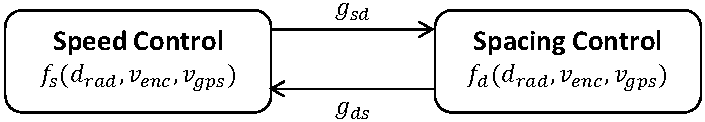
\includegraphics[width=0.48\textwidth]{image/acc_abstract_model}%
		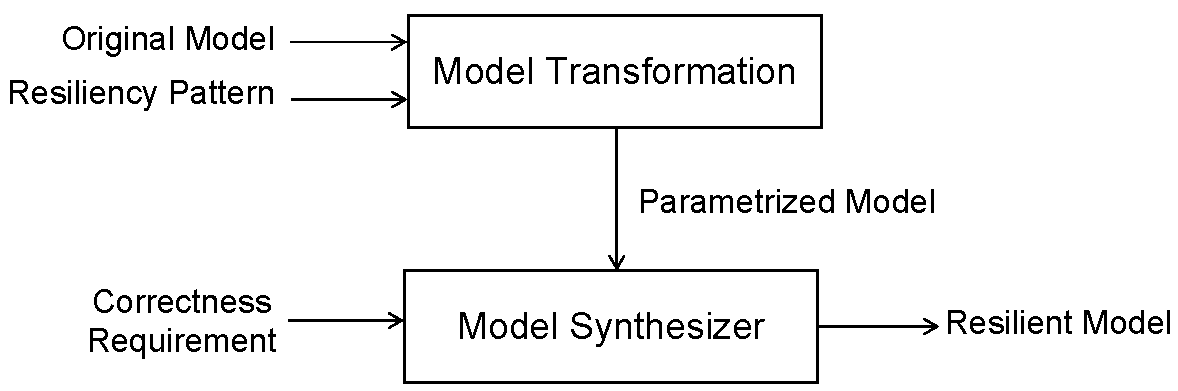
\includegraphics[width=0.46\textwidth]{image/overview}%
		%\includegraphics[trim = 17mm 85mm 17mm 0mm, clip, width=0.95\textwidth]{image/spectral_signal}%
		%\vspace{-1em}
	\caption{\toolreaffirm overview.} %{\color{red} JW: can you add dashed box containing the Model transformation and model synthesizer boxes so it is clear what we consider the inputs/outputs of \toolreaffirm, and what are internal signals.}}%
    \vspace{-1em}
	\figlabel{overview}%
	%\vspace{-1em}
\end{figure}%
Traditionally a model of a CPS consists of block diagrams describing the system architecture and a combination of state machines and differential equations describing the system dynamics~\cite{alur1995algorithmic}. Suppose a designer has initially constructed a model of a CPS that satisfies correctness requirements, but at a later stage, this correctness guarantee is invalidated, possibly due adversarial attacks on sensors, or violation of environment assumptions. Current techniques for secure-by-design systems engineering do not provide a formal way for a designer to specify a resiliency pattern to automatically repair system models based on evolving resiliency requirements under unanticipated attacks. 

In this paper, we propose a new methodology and an associated toolkit, which we call \toolreaffirm, to assist a designer in repairing the original model so that it continues to satisfy the correctness requirements under the modified assumptions. %\JW{Fixed: We haven't introduced the notion of a partial model yet -- this will be confusing to the reviewers.}
%
The proposed technique relies on designing a collection of \emph{potential edits} (or \emph{resiliency patterns}) to the original model to generate the new model whose parameters values can be determined by solving the \emph{parameter synthesis problem}. 
%\JW{Fixed: does designing a collection of resiliency patterns solve the model synthesis problem?  I don't think it does -- perhaps we can re-word this.}
%
%\JW{Fixed: This seems trivial -- why do we need a tool to do this?  Perhaps you can change "conservative" to "trivial" -- and move this sentence to after the next sentence.}
%
%
\figref{overview} shows an overview of \toolreaffirm, which contains two mains modules including a \emph{model transformation} and a \emph{model synthesizer} built on top of the falsification tool Breach~\cite{donze2010breach}.
\toolreaffirm takes the following inputs 1) the original system modeled as a Simulink/Stateflow (SLSF) diagram, 2) the resiliency pattern specified by the designer and 3) the safety requirement expressed as a Signal Temporal Logic (STL)~\cite{maler2004monitoring} formula, and then utilizes the falsification tool Breach to synthesize the repaired SLSF model that satisfies the safety requirement.

%There is currently lack of an automated mechanism that can efficiently repair the initial design and provide resilience.  
%
%
%Many significant research have been introduced to build resilient CPSs such as the approach proposed in~\cite{fitzgerald2012rigorous} that can be used to design a resilient CPS through co-simulation of discrete-event models, a modeling and simulation integration platform for secure and resilient CPS based on attacker-defender games proposed in~\cite{koutsoukos2018sure} with the corresponding testbed introduced in~\cite{neema2018integrated}, and the resilience profiling of CPSs presented in~\cite{jackson28resilience}. Although these approaches can leverage the modeling and testing for a resilient CPS, they do not offer a model repair mechanism as well as a generic approach to design a resiliency pattern when vulnerabilities are discovered. In most of the case, a designer needs to rebuild the system from scratch, which requires a lot of time and efforts.
%
%
 %Moreover, there is a lack of a generic method for a designer to specify a resiliency pattern.  
%
 %
%
%

%Suppose the designer has initially constructed a model of a CPS that satisfies correctness requirements, but at a later stage, this correctness guarantee is invalidated, possibly due to the emergence of new requirements, or adversarial attacks on sensors, or violation of environment assumptions. 
%
%

 %For example, a trivial way ensuring safety upon encountering an unexpected or hazardous situation is to hand over control to a baseline safety controller. 
%
%\OS{Fixed: "known" may not be the right word.  Maybe "specified by the designer."}  
%
%The resilient version generated by \toolreaffirm may have additional modes of operation as well as new transitions between different modes, and as a result, has resilient behaviors.
%

%The designer can construct a resiliency pattern to repair the original model based on the feedback derived from a counterexample generated by the \emph{falsification} tool embedded within \toolreaffirm. 
%%
%%\OS{Fixed: I don't quite understand the message of this sentence.  Are behaviors resilient because they are derived from a counterexample?  They are not added due to the counterexample.  On the contrary, counterexamples remove some behaviors added by the pattern because they do not fix the problem.}
%%
%Since a counterexample characterizes undesirable, or \emph{shall not},\OS{This is language specific to CASE.  Not everyone will understand.} situations, it can naturally describe how a system should respond when a particular sensor fails, or a previously unanticipated attack is identified. The model synthesizer within \toolreaffirm can automatically integrate such a counterexample with state-machine based models thus allowing an incremental design to support resiliency.
%
%
To allow a designer to specify resiliency patterns we have developed a new \emph{model transformation language} for hybrid systems, called HATL (Hybrid Automata Transformation Language).
%\IL{Expand it here since this is the first time HATL is used}
A HATL script is a sequence of statements that describe the modifications over the structure of hybrid systems modeled as hybrid automata~\cite{alur1995algorithmic}.  Examples of edits to a model include creating new modes of operations, duplicating modes, adding transitions, modifying switching conditions, and substitution of state variables in flow equations. 
%
The proposed language allows the designer to write a resiliency pattern in a generic manner, programmatically modify the initial design without knowing the internal structures of a system. The interpreter of HATL is implemented in Python with the backend is extensible for the translations to different modeling frameworks of hybrid systems. The current implementation of HATL supports the translation of a HATL script to an equivalent Matlab script that can perform the model transformation for Stateflow models.
%
To the best of our knowledge, this transformation language is the first effort to design a programmable pattern to repair CPS models for improving resiliency.
%
%\OS{Fixed: I would rephrase this to make the connection with the earlier statement that a pattern needs to be specified as input. Consider "to allow the designer to specify a resilience pattern, we have developed..."}
%For example, a conservative way ensuring safety upon encountering an unexpected or hazardous situation is to hand over control to a baseline safety controller.


For evaluation, we apply \toolreaffirm to automatically synthesize the repaired models for two proof-of-concept case studies in the domains of automotive control and smart power systems. The first case study is a simplified model of an adaptive cruise control (ACC) system under a GPS sensor spoofing attack, and the resiliency pattern to fix the model is to ignore the GPS measurement and only use the wheel encoders, which are additional (redundant) sensors for estimating a vehicle's velocity. The synthesizer tool of \toolreaffirm automatically synthesizes the condition that triggers a switch to a copy of the model that ignores the GPS measurement. The second case study is a single-machine infinite-bus (SMIB) model, which is an approximation of a smart power grid, under a sliding-mode attack. In this case, the mitigation strategy is to increase the minimal dwell-time to avoid rapid changes between different operation modes. Thus, the resiliency pattern is adding a dwell-time variable in each mode of the model, and the minimal dwell-time can be synthesized automatically by \toolreaffirm.  
%
%
%

In summary, the main contributions of the paper are as follows.
%
\begin{enumerate}[leftmargin= 2 em]
\item the methodology to facilitate the model-based repair for improving the resiliency of CPSs against unanticipated attacks and failures,
\item the design and implementation of an extensible model transformation language for specifying resiliency patterns used to repair CPS models,
\item the end-to-end design and implementation of the toolkit, which integrates the model transformation and the model synthesis tools to automatically repair CPS models,
\item the applicability of our approach on two proof-of-concept case studies where the CPS models can be automatically repaired to mitigate practical attacks.
\end{enumerate}
%\JW{Fxied: an extensible?}
%
%We anticipate that our methodology proposed along with \toolreaffirm for automatically conducting the model repair and specifying the patterns of resiliency will be contributions of significant interest to the research community in the design of resilient CPSs. Our vision of \toolreaffirm is that a designer can incorporate the toolkit as an efficient repair mechanism in the model-based design paradigm to iteratively improve the original design for resiliency when new vulnerabilities are identified and requirements evolve.
%
%

The remainder of the paper is organized as follows.~\secref{overview} presents an overview of our proposed methodology through a simplified example of the ACC system, and introduces the architecture of \toolreaffirm.~\secref{transformation} describes our model transformation language used to design a resiliency pattern for hybrid systems.~\secref{synthesis} presents the model synthesizer of \toolreaffirm.~\secref{result} presents two case studies that illustrate the capability of \toolreaffirm in automatically repairing the original models of a) the ACC system under a GPS sensor spoofing attack and b) the smart power grid system under a sliding-mode attack.~\secref{rw} reviews the related works to \toolreaffirm.~\secref{conclude} concludes the paper and presents future research directions for the proposed work.
% \JW{Fixed a toy example ... no need to say "running" -- that will be obvious.}






%
\section{Overviews of Methodology}
\seclabel{overview}
%
%
In this section, we will explain our methodology through the running example of an adaptive control system (ACC). This system has been designed to satisfy safety requirements pertaining to vehicle spacing that varies with vehicle speed.
%which aims to safely adapt a vehicle speed
%In the following, we first present the original (legacy) system which satisfies an initial functional safety requirement. 
%
Assume that a designer has previously modeled an ACC system as a combination of the vehicle dynamics and an control module, and resiliency was not considered in the initial design. In the following, we will describe the ACC system as originally designed, its attack scenario, and an example of resilient pattern. 
%
Then, we present the structure of \toolreaffirm and demonstrate how \toolreaffirm can automatically perform a model transformation and synthesis to construct a new ACC model with resiliency. 
%
%which will (in the subsequent discussion) be adapted to satisfy a resiliency requirement.
%
%

\subsection{Original ACC Model}
\begin{figure}[t!]%
	\centering%
	\begin{adjustbox}{max size={0.99\columnwidth}{0.75\textheight}}%
	\begin{tikzpicture}[>=stealth',shorten >=1pt,auto,node distance=8cm,font=\Large]
		%\tikzstyle{every state}=[minimum size=3cm,font=\normalsize]
		\tikzstyle{every state}=[font=\Large,rectangle,rounded corners, minimum size=5cm]
		\node[state] (speed)      			{\makecell[c]{$\textbf{Speed Control}$\\\\
		$\begin{aligned}
		\dot{d} & = \vlead - v \nonumber \\
		\dot{v} & = 2\vlead - v - \hat{v} \nonumber \\
		\dot{\hat{d}} & = \vlead - \hat{v} + 10(\drad-\hat{d})\nonumber \\
		\dot{\hat{v}} & = 2\vlead - 3\hat{v} + \frac{1}{2} (\ngps + \nenc) \nonumber\\
		\end{aligned}$\\\\
		$\hat{d} \geq 10 + 2\hat{v}$
		}};
		\node[state] (space) [right of=speed]	{\makecell[c]{$\textbf{Spacing Control}$\\\\
		$\begin{aligned}
		\dot{d} & = \vlead - v \nonumber \\
		\dot{v} & = 2\vlead - v - \hat{v} -\frac{1}{4}(10 + 2\hat{v}-\hat{d}) \nonumber \\
		\dot{\hat{d}} & = \vlead - \hat{v} + 10 (\drad-\hat{d})\nonumber \\
		\dot{\hat{v}} & = 2\vlead - 3\hat{v} + \frac{1}{2} (\ngps + \nenc) -\frac{1}{4}(10 + 2\hat{v}-\hat{d}) \nonumber\\
		\end{aligned}$\\\\
		$\hat{d} < 10 + 2\hat{v}$
		}};
		
		\node (speedtospace) [above=6mm of speed,xshift=40mm]{\makecell[c]{$\hat{d} < 10 + 2\hat{v}$}};
		%$\dot{d} = \vlead - v$\\$\dot{v} = 2\vlead - v - \hat{v} -\frac{1}{4}(10 + 2\hat{v}-\hat{d}$\\$\dot{\hat{d}} = \vlead - \hat{v} + 10(\drad-\hat{d})$\\$\dot{\hat{v}} = 2\vlead - 3\hat{v} + \frac{1}{2} (\ngps + \nenc) -\frac{1}{4}(10 + 2\hat{v}-\hat{d}$}}; 
		
		\node[coordinate] (c1) [above=5mm of speed.north] {};
		\node[coordinate] (c2) [above=5mm of space.north] {};
		\draw[->]			(speed.north) -- (c1) -- (c2) to (space.north);
		
		\node (spacetospeed) [below=6mm of space,xshift=-40mm]{\makecell[c]{$\hat{d} \geq 10 + 2\hat{v}$}};

		\node[coordinate] (c3) [below=5mm of space.south] {};
		\node[coordinate] (c4) [below=5mm of speed.south] {};
		\draw[->]			(space.south) -- (c3) -- (c4) to (speed.south);
		%
		%\path[->]			(speed.north) edge[bend left] node{\makecell[c]{$\mathit{OD} \leq \mathit{OD}_t \wedge t_m \geq t_\text{mOn} $\\$t_m' := 0$}} (space.north); 
		%\path[->]			(space.south)	edge[bend left] node{\makecell[c]{$\mathit{OD} \geq \mathit{OD}_t \wedge t_m \geq t_\text{mOff} $\\$t_m' := 0$}} (speed.south); 
	\end{tikzpicture}%
	\end{adjustbox}%
	\caption{Original ACC model}%
	\figlabel{original}%
\end{figure}

%To illustrate and motivate our proposed approach, this subsection presents a case study of a control system that aims to safely adapt a vehicle speed, namely, an adaptive cruise control (ACC) system. 

%
%\noindent
%{\bf Original ACC Model.}
The original ACC system operates in two modes: \emph{speed control} and \emph{spacing control}. In speed control, the host car travels at a driver-set speed. In spacing control, the host car aims to maintain a safe distance from the lead car. The ACC system decides which mode to use based on the real-time sensor measurements. For example, if the lead car is too close, the ACC system switches from speed control to spacing control. 
%
Similarly, if the lead car is further away, the ACC system switches from spacing control to speed control. In other words, the ACC system makes the host car travel at a driver-set speed as long as a safe distance is maintained.

The vehicle has two states in which $d$ is the distance to the lead car, and $v$ is the speed of the host vehicle. These states evolve according to $\dot{d} = \vlead - v$ and $\dot{v} = -v + u$, 
%
where $\vlead$ is the speed of the lead vehicle  and $u$ is the control input.  In this example, we assume that the lead vehicle speed is known exactly (\eg it is communicated between vehicles). Conceptually, the dynamics for $d$ represent that the derivative of the relative distance is the difference between the lead vehicle speed and the host vehicle speed.  The dynamics for the host vehicle speed indicate that as the vehicle speed increases, it takes more acceleration (\ie force) provided by the controller (\ie engine) to maintain speed. 

An ACC equipped vehicle has sensors that measure its velocity $v$ via noisy wheel encoders, $\venc = v + \nenc$, and a noisy GPS sensor, $\vgps = v+\ngps$, where $\nenc$ and $\ngps$ denote the encoder and GPS noisy, respectively. 
%
%
Additionally, the ACC system has a radar sensor that measures the distance to a (potential) lead vehicle, $\drad = d+\nrad$. 
%
To design a control law, we need to estimate the state of the vehicle (\ie we need an estimate of $d$ and $v$, which we will call $\hat{d}$ and $\hat{v}$). To estimate the distance and velocity, we employ state estimators
%
\begin{align}
\dot{d} & = \vlead - \hat{v} + 10(\drad - \hat{d}) \nonumber \\
\dot{v} & = -\hat{v} + u +  \frac{1}{2} ((\vgps + \venc) - \hat{v}) \nonumber
\end{align}
%
%
To implement a controller, a control law based on the state estimates in speed and distance control modes are given: 

\begin{align}
u_s & = \vlead - (\hat{v}-\vlead) \nonumber \\
u_d & = \vlead - (\hat{v}-\vlead) - \frac{1}{4} (d_{ref} - \hat{d}) \nonumber
\end{align}
%
%
where $u_s$ is the control law in the speed mode, $u_d$ is the control law in the spacing mode, and $d_{ref} = 10 + 2\hat{v}$. These control laws incorporate a reference velocity $\vlead$, which can be thought of as constant gain that depends on the lead (or desired) vehicle velocity, while the other terms depend on the deviation of the lead vehicle and and ego vehicle states. Switching between modes is handled by monitoring the state estimates. The designer models the complete ACC system (including vehicle dynamics) as a hybrid system, illustrated in \figref{original}. Here, the transition from speed control to spacing control occurs when the estimate of the distance is less than twice the estimated safe distance, \ie $\hat{d} < 10 + 2\hat{v}$. A similar condition is provided for transitioning from spacing control to speed control, \ie $\hat{d} \geq 10 + 2\hat{v}$. 
%
%
 %Next we add a new resilience requirement that is determined to be violated by the original system. Finally, we adapt the original system such that the resilience requirement is satisfied.

\subsection{Safety Violation under GPS Sensor Attack}
%\noindent
%{\bf Attack Scenarios.}
%
In this example, the functional safety specification of the ACC system is specified that $d$ should always be greater than $d_{safe} = 5 + v$. Assume that the designer has verified the ACC system safety requirement under the scenario when $d(0) \geq 20$, $v(0) \leq 30$, $|d(0) - \hat{d}(0)| \leq 1$, $|v(0) - \hat{v}(0)| \leq 1$ , $\vlead \geq 0$, $|\nenc| \leq 0.05$ and $|\ngps| \leq 0.05$.
%
After designing the initial ACC system, it is determined that the GPS sensor can be \emph{spoofed} \cite{tippenhauer2011requirements, kerns2014unmanned}. GPS spoofing occurs when incorrect GPS packets (possibly sent by a malicious attacker) are received by the GPS receiver. In the ACC system, this allows an attacker to arbitrarily change the GPS velocity measurement. 
%
Thus, a new scenario occurs when the assumption that $|\ngps| \leq 0.05$ is omitted, and the new assumption is $|\ngps| \leq \infty$.
As a result, the safety specification could be violated under the GPS sensor attacks, and a designer needs to repair the original model with a resilient pattern. 

\subsection{Example of Resilient Pattern}
%
%
To provide resilience against the GPS attacks, a potential strategy is to ignore the GPS value in resilient modes and use only the wheel encoders to estimate velocity. Since the ACC system has redundancy in the sensory information of its estimated velocity, the model synthesizer can repair the model by replacing the GPS velocity measurement with the wheel encoder velocity measurement when the GPS measurement significantly deviates from the wheel encoder measurement.
%
%
Thus, the proposed fix then is first to create a resilient copy of the original model where the controller simply ignores the GPS reading as it can no longer be trusted. Then, adding new transitions from the legacy speed and spacing modes of the original model to the new resilient speed and spacing modes of the copy that uses only the wheel encoder as a velocity measurement source. We note that this transformation is generic, that is, it can be applied in a uniform manner to any given model simply by creating a duplicate version of each original mode and transition, copying the dynamics in each mode, but without a reference to the variable $\ngps$. 

%
%
\begin{figure}[!t]%frame=none,
\begin{lstlisting}[basicstyle=\ttfamily\footnotesize, numbers=none]
model = getModelByName("ACC") # retrieve the ACC model
model_copy = copyModel(model) # make a model copy 
	
# start a transformation  
addParam(model,"theta") # add new parameter theta
	
formode m = model.Mode {
		m_copy = addState(model,m)
		replace(m_copy.flow,"ngps","nenc")
		addTransition(model,m,m_copy,"abs(ngps-nenc)>theta")
}

fortran t = model_copy.Trans {
		# get source and destination modes of transition t
		src = t.source	
		dst = t.destination 
		# retrieve copies of source and destination modes 
		src_copy = getCopyState(model,src)  
		dst_copy = getCopyState(model,dst) 
		addTransition(model,src_copy,dst_copy,t.guard)
}
# end of the transformation
\end{lstlisting}
\caption{An example of a resilient pattern written as a HATL script for the ACC system.}%
\figlabel{examplecode}%
	%\vspace{-0.5em}%
\end{figure}
%
%


~\figref{examplecode} shows an example of a resilient pattern written as a transformation script that specifies a transformation from the original ACC model shown in~\figref{original} to the parametrized model that enables resilience. 
%
In this script, we first create a copy of the original model. Next, we iterate over each mode of the model by calling the \emph{formode loop}, make a copy with replacing the variable $\ngps$ by $\nenc$, and then add a new transition from the original mode to the copied mode with a new guard condition. This guard condition is a constraint specified over the difference between $\ngps$ by $\nenc$ and a new parameter $\theta$, which is added into the model using a function call \emph{addParam}.
%
%
Observe that while it would be possible to use only the wheel encoder all the time, a better velocity estimate must be obtained by using an average velocity measurement (from both the GPS and wheel encoders) when the GPS sensor is performing within nominal specifications. The main analysis question is when should the model switch from original copy to this resilient copy.  In this example, we model this switching condition as $|\ngps -\nenc| \geq \theta$, where $\theta$ is an unknown parameter. 




\subsection{REAFFIRM Toolkit}
%
Our \toolreaffirm prototype for the model-based design and repair with resiliency consists of two tools, corresponding to a \emph{model transformation} and a \emph{model synthesizer} as shown in \figref{overview}.
%
\begin{itemize}[leftmargin= 2 em]
	\item \textbf{Model Transformation} takes a given initial model and a resiliency pattern, and generates a partial model that contains \emph{holes}, that is, parameters for which values need to be determined to ensure that the correctness requirements are satisfied. The resiliency pattern captures a generic way of transforming models that corresponds to commonly known mitigation strategies. The parameters in the incomplete model correspond to unknown switching conditions, or unknown assignments in variable updates, or even unknown coefficients in controller dynamics. The model is specified using the MathWorks Simulink/Stateflow (SLSF) format, and the correctness requirement is specified in the temporal logic Signal Temporal Logic (STL) that is widely used in tools for verification for cyber-physical systems~\cite{maler2004monitoring}. The resiliency pattern can be specified as a \emph{model transformation script} that operates on the internal representation of SLSF models specifying the desired transformation in a generic way. As an example, for a system that contains a nominal controller and a safety controller, a resiliency pattern can be specified as a transition from nominal controller to safety controller.
%
\item \textbf{Model Synthesizer} takes a parameterized model (SLSF) and a correctness requirement (STL formula) as inputs and outputs a completed model with parameter values instantiated so as to satisfy the correctness requirements.  Internally, the tool utilizes an open-source model falsification tool---Breach~\cite{donze2010breach}, to check an SLSF model against the specification. The counterexamples returned by this falsification tool are used to determine values for the desired parameters. At the end of a falsification loop, the completed model produced by \toolreaffirm, compared to the partial behavior model, can have additional modes of operation as well as new transitions between different modes, and as a result has resilient behaviors specified in the resilient patterns.
\end{itemize}
%
%
%
%
\begin{figure}[t!]%
	\centering%
    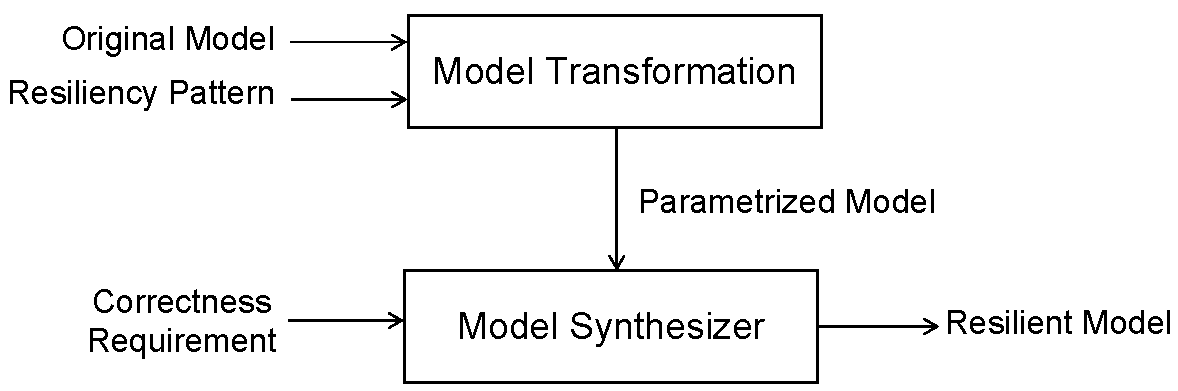
\includegraphics[width=0.48\textwidth]{image/overview}%
		%\includegraphics[trim = 17mm 85mm 17mm 0mm, clip, width=0.95\textwidth]{image/spectral_signal}%
		%\vspace{-1em}
	\caption{\toolreaffirm Overview.}%
	\figlabel{overview}%
	%\vspace{-1em}
\end{figure}%
%
%

To provide a resilience for the ACC example, the transformation tool of \toolreaffirm will take the original ACC model shown in ~\figref{original} and the transformation script shown in \figref{examplecode}, and then output the \emph{parameterized} model shown in \figref{updated}, where the variable $\ngps$ is replaced by the variable $\nenc$ in the resilient speed and spacing control modes, and the value of $\theta$ needs to be determined. Next, the model synthesizer of \toolreaffirm takes the parameterized ACC model, the safety requirement encoded as an STL formula $\Box_{[0, \infty]} (d[t] < 5 + v[t])$, and the specific range of $\theta$, and then calls the synthesizer to determine the best $\theta$ which ensures the final model will always satisfy the safety requirement. If the tool cannot find any value of $\theta$ over a given range, it will suggest a designer to either search over a wider parameter range or try a different resilient pattern.   
%
%

\begin{figure}[t!]%
	\centering%
	\begin{adjustbox}{max size={0.99\columnwidth}{0.75\textheight}}%
	\begin{tikzpicture}[>=stealth',shorten >=1pt,auto,node distance=8cm,font=\Large]
		%\tikzstyle{every state}=[minimum size=3cm,font=\normalsize]
		\tikzstyle{every state}=[font=\Large,rectangle,rounded corners, minimum size=5cm]
		\node[state] (speed)      			{\makecell[c]{$\textbf{Speed Control}$\\\\
		$\begin{aligned}
		\dot{d} & = \vlead - v \nonumber \\
		\dot{v} & = 2\vlead - v - \hat{v} \nonumber \\
		\dot{\hat{d}} & = \vlead - \hat{v} + 10(\drad-\hat{d})\nonumber \\
		\dot{\hat{v}} & = 2\vlead - 3\hat{v} + \frac{1}{2} (\ngps + \nenc) \nonumber\\
		\end{aligned}$\\\\
		$\hat{d} \geq 10 + 2\hat{v}$
		}};
		\node[state] (space) [right of=speed]	{\makecell[c]{$\textbf{Spacing Control}$\\\\
		$\begin{aligned}
		\dot{d} & = \vlead - v \nonumber \\
		\dot{v} & = 2\vlead - v - \hat{v} -\frac{1}{4}(10 + 2\hat{v}-\hat{d}) \nonumber \\
		\dot{\hat{d}} & = \vlead - \hat{v} + 10 (\drad-\hat{d})\nonumber \\
		\dot{\hat{v}} & = 2\vlead - 3\hat{v} + \frac{1}{2} (\ngps + \nenc) -\frac{1}{4}(10 + 2\hat{v}-\hat{d}) \nonumber\\
		\end{aligned}$\\\\
		$\hat{d} < 10 + 2\hat{v}$
		}};
		
		\node[state] (res_speed) [below of=speed]  {\makecell[c]{$\textbf{Resilient Speed Control}$\\\\
		$\begin{aligned}
		\dot{d} & = \vlead - v \nonumber \\
		\dot{v} & = 2\vlead - v - \hat{v} \nonumber \\
		\dot{\hat{d}} & = \vlead - \hat{v} + 10(\drad-\hat{d})\nonumber \\
		\dot{\hat{v}} & = 2\vlead - 3\hat{v} + \frac{1}{2} (\nenc + \nenc) \nonumber\\
		\end{aligned}$\\\\
		$\hat{d} \geq 10 + 2\hat{v}$
		}};
		
		\node[state] (res_space) [right of=res_speed]	{\makecell[c]{$\textbf{Resilient Spacing Control}$\\\\
		$\begin{aligned}
		\dot{d} & = \vlead - v \nonumber \\
		\dot{v} & = 2\vlead - v - \hat{v} -\frac{1}{4}(10 + 2\hat{v}-\hat{d}) \nonumber \\
		\dot{\hat{d}} & = \vlead - \hat{v} + 10 (\drad-\hat{d})\nonumber \\
		\dot{\hat{v}} & = 2\vlead - 3\hat{v} + \frac{1}{2} (\nenc + \nenc) -\frac{1}{4}(10 + 2\hat{v}-\hat{d}) \nonumber\\
		\end{aligned}$\\\\
		$\hat{d} < 10 + 2\hat{v}$
		}};
		
		
		\node (speedtospace) [above=6mm of speed,xshift=40mm]{\makecell[c]{$\hat{d} < 10 + 2\hat{v}$}};
		%$\dot{d} = \vlead - v$\\$\dot{v} = 2\vlead - v - \hat{v} -\frac{1}{4}(10 + 2\hat{v}-\hat{d}$\\$\dot{\hat{d}} = \vlead - \hat{v} + 10(\drad-\hat{d})$\\$\dot{\hat{v}} = 2\vlead - 3\hat{v} + \frac{1}{2} (\ngps + \nenc) -\frac{1}{4}(10 + 2\hat{v}-\hat{d}$}}; 
		
		\node[coordinate] (c1) [above=5mm of speed.north] {};
		\node[coordinate] (c2) [above=5mm of space.north] {};
		\draw[->]			(speed.north) -- (c1) -- (c2) to (space.north);
		
		\node (spacetospeed) [below=6mm of space,xshift=-40mm]{\makecell[c]{$\hat{d} \geq 10 + 2\hat{v}$}};

		\node[coordinate] (c3) [below=5mm of space.south] {};
		\node[coordinate] (c4) [below=5mm of speed.south] {};
		\draw[->]			(space.south) -- (c3) -- (c4) to (speed.south);
		
		\node (res_speedtospace) [above=6mm of res_speed,xshift=40mm]{\makecell[c]{$\hat{d} < 10 + 2\hat{v}$}};
		%$\dot{d} = \vlead - v$\\$\dot{v} = 2\vlead - v - \hat{v} -\frac{1}{4}(10 + 2\hat{v}-\hat{d}$\\$\dot{\hat{d}} = \vlead - \hat{v} + 10(\drad-\hat{d})$\\$\dot{\hat{v}} = 2\vlead - 3\hat{v} + \frac{1}{2} (\ngps + \nenc) -\frac{1}{4}(10 + 2\hat{v}-\hat{d}$}}; 
		
		\node[coordinate] (c5) [above=5mm of res_speed.north] {};
		\node[coordinate] (c6) [above=5mm of res_space.north] {};
		\draw[->]			(res_speed.north) -- (c5) -- (c6) to (res_space.north);
		
		\node (res_spacetospeed) [below=6mm of res_space,xshift=-40mm]{\makecell[c]{$\hat{d} \geq 10 + 2\hat{v}$}};

		\node[coordinate] (c7) [below=5mm of res_space.south] {};
		\node[coordinate] (c8) [below=5mm of res_speed.south] {};
		\draw[->]			(res_space.south) -- (c7) -- (c8) to (res_speed.south);
		
		\node[coordinate] (c9) 	[left=5mm of speed.south] {};
		\node[coordinate] (c10) [left=5mm of res_speed.north] {};
		\node[coordinate] (c11) [right=5mm of space.south] {};
		\node[coordinate] (c12) [right=5mm of res_space.north] {};
		
		%\draw[->]			(speed.south)[right=1mm to (res_speed.north);
		%\draw[->]			(space.south) to (res_space.north);
		
		\path[->]			(c9) edge node[xshift=-29mm]{\makecell[c]{$|\ngps -\nenc| \geq \theta$}}(c10); 
		\path[->]			(c11) edge node[xshift=1mm]{\makecell[c]{$|\ngps -\nenc| \geq \theta$}} (c12); 
		
		%
		%\path[->]			(speed.north) edge[bend left] node{\makecell[c]{$\mathit{OD} \leq \mathit{OD}_t \wedge t_m \geq t_\text{mOn} $\\$t_m' := 0$}} (space.north); 
		%\path[->]			(space.south)	edge[bend left] node{\makecell[c]{$\mathit{OD} \geq \mathit{OD}_t \wedge t_m \geq t_\text{mOff} $\\$t_m' := 0$}} (speed.south); 
	\end{tikzpicture}%
	\end{adjustbox}%
	\caption{Updated Resilient ACC model}%
	\figlabel{updated}%
\end{figure}

%
%\vspace{-0.5em}
%\section{Preliminaries}
\seclabel{pre}


%\subsection{Protocol Completion}



\subsection{Parameterized Hybrid Input-Output Automata}
Hybrid automata~\cite{alur1995algorithmic} are a modeling formalism popularly used to model CPSs which include both continuous dynamics and discrete state transitions. A hybrid automaton is essentially a FSM extended with a set of real-valued variables evolving continuously over intervals of real-time~\cite{alur1995algorithmic}. In our approach, we consider a CPS that can be formally represented as parametrized hybrid input-output automata (PHIOA)\footnote{In this paper, we only consider \emph{deterministic} systems, where the system produces the same output for a given input. Note the contrast with {\em stochastic} systems in which one or more elements of the system have randomness associated with them; for example, the value of some system parameter may be extracted from a probability distribution. As a result, the stochastic system may yield different outputs for a given input.}, where the parameters representing arbitrary values which do not change during one system execution~\cite{frehse2008counterexample, schwarz2011modelling}. 
%\noindent
%{\bf Hybrid Automata.}
\begin{definition}[Parameterized Hybrid Input-Output Automata]
A $\AutomatonH$ is a tuple, $\AutomatonH$ $\deq$ $\langle$$\Varset$, $\Locset$,  $\Transset$, $\Trajectoryset$, $\Initset$$\rangle$, where
%
%\begin{itemize}[leftmargin= 1 em]
\begin{itemize}[leftmargin= 2em]
%\begin{inparaenum}[(a)]
%
%
%\item $\mathtt{Lab}$: a finite set of synchronization labels,
%
\item $\Varset$: the finite set of $n$ continuous, real-valued variables; we have $\Varset = \X \cup \P$, where $\X \in \Realn$ is the set of $n$ state variables and $\P\in\Realp$ is the set of $p$ parameters. Moreover, $\Varset$ is the disjoint of the set of input variables $\I$ and the set of output variables $\O$, and $\Q \deq \Locset \times \Realn$ is the state space.
%
\item $\Locset$: the finite set of discrete modes.  For each mode $\mode \in \Locset$, $\mode.\inveg \subseteq \Real^{n+p}$ denotes the invariant of mode $\mode$, and $\mode.\floweg \subseteq \Realn$ describes the continuous dynamics.
%and $\forall x \in \Varset$, a \emph{valuation} $\val{x} \in \Real$ is a function mapping $x$ to a point in its type---here, $\Real$; and $\Q \deq \Locset \times \Realn$ is the state space. 
%\item $\VarInput$: the set of input variables. 
%\item $\VarOutput$: the set of output variables.
%
%\item $\Parameterset$: the set of parameters. 
%
%
%
%\item $\Invset$: the finite set of invariants. For each mode $\mode \in \Locset$, $\mode.\inveg \subseteq \Realn$ denotes the invariant $\inveg \in \Invset$ of mode $\mode$. 
%
%\item $\Flowset$: the finite set of ordinary differential inclusions. For each $\floweg\in \Flowset$, $\mode.\floweg \subseteq \Realn$ describes the continuous dynamics in each mode $\mode \in \Locset$.
%
\item $\Transset$: the finite set of transitions between modes.
%
Each transition is a tuple $\tau \deq \tuple{\mode, \mode', \guard, \reset}$, where $\mode$ is a source mode and $\mode'$ is a target mode that may be taken when a guard condition $\guard$ is satisfied, and the post-state is updated by an update map $\reset$.
%
\item $\Trajectoryset$: a finite set of continuous trajectory models the valuations of state variables over an interval of real time $[0, T]$. Let $\val{x}_t$ be the valuations of variable $x$ at time points $t$, $\forall t \in [0, T]$, $\forall x \in \X$, $\exists m \in \Locset$, a trajectory $\gamma \in \Trajectoryset$ is a mapping function $\gamma: [0, T] \rightarrow \val{\X}$ such that:
\begin{itemize}
\item $\val{x}_t = \val{x}_0 + \int_{\delta = 0}^{t} m.\floweg(x) d\delta$, and %where $\Delta_0$ is a valuation of variable $x$ at $t = 0$
\item $\val{x}_t \models m.\inveg$ for all $t \in [0, T]$.
%
\end{itemize}
%
\item $\Initset$ is an initial condition, and $\Initset \subseteq \Q$.
%\end{inparaenum}
\end{itemize}
\end{definition}
% 
We use the dot (.) notation to refer to different components of tuples \eg $\AutomatonH.\Transset$ refers to the transitions of automaton $\AutomatonH$ and $\tau.\guard$ refers to the guard of a transition $\tau$.
%\end{definition}

The semantics of a PHIOA $\AutomatonH$ are defined in terms of executions, which are sequences of states. Given the set of parameter value $P_0\in \Realp$, an \emph{execution} of $\AutomatonH$ w.r.t $P_0$ is a sequence $\pi_{P_0} \deq \s_0 \rightarrow \s_1 \rightarrow \s_2 \rightarrow \dotline$, where $\s_0 \in \Initset$ is an initial state, and $\s_i \rightarrow \s_{i+1}$ is the update from the current-state $\s_i$ to the post-state $\s_{i+1}$, that is specified by the transition relations of $\AutomatonH$ including:
\begin{inparaenum}[(a)]
\item a discrete transition that describes the instantaneous state update, or
\item a continuous trajectory that represents the state update over a real time interval (see \cite{david2010timed,frehse2008counterexample} for more details).
\end{inparaenum}
%
%
We say a state $\s_k$ is \emph{reachable} from an initial state $\s_0$ w.r.t $P_0$ if there exists an execution $\pi_{P_0} \deq \s_0 \rightarrow \s_1 \rightarrow \dotline \rightarrow \sk$. We denote $\exec(\AutomatonH)$ and $\reach(\AutomatonH)$  as the set of all executions and the set of all reachable states of $\AutomatonH$, respectively.

\begin{definition}[Verification Problem]
Given a safety specification $\varphi$ which is a formula over $\Locset$ and $\Varset$ that describes a set of states $\ds{\varphi} \subseteq \Q$, where $\ds{\cdot}$ is the set of states satisfying $\varphi$, a PHIOA automaton $\AutomatonH$ satisfies the specification $\phi$, denoted $\AutomatonH \models \phi$ if and only if $\reach(\AutomatonH) \subseteq \ds{\varphi}$.
\end{definition}

If a PHIOA automaton $\AutomatonH$ does not satisfy a safety specification $\varphi$, there exists an execution $\pi_{P_0} \in \exec(\AutomatonH)$ w.r.t to some parameter values $P$ in which some state $\si \in \pi_{P_0}$ violates $\varphi$, \ie $\si \notin \ds{\varphi}$. We call such an execution as a \emph{counterexample}. Searching for a counterexample of $\AutomatonH$ with respect to a safety property $\varphi$ is considered as solving the falsification problem of $\AutomatonH$.
 

\begin{definition}[Falsification Problem]
Given a PHIOA automaton $\AutomatonH$ and a safety specification $\varphi$, a falsification problem is to find the sets of input parameters values $P_0$ of $\P$ and initial conditions of state variables $X_0$ of $\X$ that generates a counterexample driving the automaton $\AutomatonH$ toward a violation of $\varphi$.
\end{definition}

As a counterexample returned by addressing the falsification problem illustrates unexpected behaviors of a system, it reveals how a system should be repaired to mitigate an adversarial attack or accommodate a system change. The designer then either develops a corresponding pattern or search through the space of potential edits to transform an original system to a new system that produces no counterexample with respect to the given safety specification. %Let $\varphi$,$\pi_P \in \exec(\AutomatonH)$ be a counterexample returned from solving the falsification problem of $\AutomatonH$ against $\varphi$ w.r.t the set of input parameters values $P$, the designer can specify a resilient pattern $\Gamma$ based on $\pi_P$,   

\begin{definition}[Model Transformation Problem]
Given an initial PHIOA automaton $\AutomatonH$ with a set of parameter $\P$, a safety specification $\varphi$ such that $\AutomatonH \not\models \varphi$, and a resilient pattern $\Gamma$, addressing the model transformation problem of $\AutomatonH$ is to determine a new PHIOA automaton $\tilde{\AutomatonH} \deq \Gamma(\AutomatonH)$ such that $\tilde{\AutomatonH}\models\varphi$.
\end{definition}


%\begin{definition}[Model Synthesis Problem]
%Given an transformed PHIOA automaton $\tilde{\AutomatonH}$ and a safety specification, let $\varphi$,$\pi_P \in \exec(\AutomatonH)$ be a counterexample returned from solving the falsification problem of $\AutomatonH$ against $\varphi$ w.r.t the set of input parameters values $P$, and a resilient pattern $\Gamma$, addressing the model synthesis problem of $\AutomatonH$ is to determine a new PHIOA automaton $\tilde{\AutomatonH} \deq \Gamma(\AutomatonH,\pi_P)$ such that $\tilde{\AutomatonH}\models\varphi$.
%\end{definition}

In this paper, the transformed automaton $\tilde{\AutomatonH}$ contains a set of parameter $\P'= \P \cup \P_s$ in which the values of $\P_s$ need to be synthesized to ensure the system is correct. 

%\begin{definition}[Model Synthesis Problem]
%Given a transformed PHIOA automaton $\tilde{\AutomatonH}$ with set of parameter $\P_s$ and a safety specification $\varphi$, the model synthesis problem of $\AutomatonH$ is to determine a set of instance values $P_0$ of $\P'$ such that $\tilde{\AutomatonH} \models\varphi$.
%\end{definition}


%\begin{definition}[Model Synthesis Problem]
%Given an transformed PHIOA automaton $\tilde{\AutomatonH}$ and a safety specification, let $\varphi$,$\pi_P \in \exec(\AutomatonH)$ be a counterexample returned from solving the falsification problem of $\AutomatonH$ against $\varphi$ w.r.t the set of input parameters values $P$, and a resilient pattern $\Gamma$, addressing the model synthesis problem of $\AutomatonH$ is to determine a new PHIOA automaton $\tilde{\AutomatonH} \deq \Gamma(\AutomatonH,\pi_P)$ such that $\tilde{\AutomatonH}\models\varphi$.
%\end{definition}

%Recently, falsification tools such as Breach~\cite{donze2010breach} and S-taliro~\cite{annpureddy2011s} have been introduced and successfully applied to falsify complex automotive control systems. 



\subsection{Continuous-time Stateflow Chart}
In this paper, we model a PHIOA as a \emph{continuous-time} Stateflow chart, which is a commercial modeling language for hybrid systems integrated within MathWorks Simulink.
%
Continuous-time Stateflow chart\footnote{In this paper, we focus only on continuous-time Stateflow diagram that does not include hierarchical states.} supplies methods for engineers to quickly model as well as efficiently refine, test, and generate code for hybrid systems. In a Stateflow diagram, a designer can specify different data types including continuous state variables, parameters, inputs, and outputs of the model, and define the discrete structures similar to a PHIOA.
%
While the syntactic components of a continuous-time Stateflow chart are described similar to a hybrid automaton, there are slight differences between their semantics as a Stateflow diagram is deterministic and has urgent transitions with priorities. Intuitively, transitions in a Stateflow model is triggered as soon as the transition guard condition is satisfied, while a hybrid automaton can stay at the current mode as long as its invariant still holds. To overcome this gap, a recent work proposed in~\cite{bak2017hybrid} provides an equivalent translation for both classes of deterministic and non-deterministic hybrid automata to Stateflow diagrams. Other significant research have been done to translate back and forth between hybrid automata and Simulink/Stateflow models~\cite{alur2008symbolic,manamcheri2011step,minopoli2016sl2sx}.
%

\subsection{Breach}
%
%
In our proposed methodologies, we incorporated Breach into the model synthesizer of \toolreaffirm as an analysis mechanism to search for the counterexamples of hybrid systems. Given a PHIOA modeled as a continuous-time Stateflow chart, an STL specification represented the safety property, and some parameter ranges, Breach~\cite{donze2010breach} can perform an optimized search over parameter domains to find parameter values that cause the system violating the given STL specification. On the other hand, Breach can compute the sensitivity of execution traces to the initial conditions, which can be used to obtain completeness results by performing systematic simulations. We note that although falsification cannot completely prove the system correctness, it can efficiently find bugs existing in the initial design of CPS that are too complex to be formally verified~\cite{kapinski2015simulation}. These bugs are essential for an engineer to specify resilient patterns to repair the model. 
%
Moreover, the general problem of verifying a CPS modeled as a hybrid system is proved to be \emph{undecidable}~\cite{henzinger1995s}. Instead, the falsification algorithms embedded within Breach are scalable and work properly for black-box hybrid systems with different classes of dynamics.
%
Thus, in practice, engineers prefer to use counterexamples obtained by a falsification tool to refine their design. Our prototype \toolreaffirm utilizes the advantages of Simulink/Stateflow modeling framework and the falsification tool Breach to design a resilient pattern and perform the model synthesis for a resilient CPS.
%Since Mathworks Simulink/Statflow is a well-established modeling framworke for CPSs,
%\subsection{Falsification}

%To perform a model synthesis for CPS, a general approach would be to formally specify safety properties of a CPS that protect the system against possible adversarial attacks using formalisms such as signal temporal logic (STL)~\cite{maler2004monitoring} and to then iteratively improve the design using \emph{falsification}~\cite{nghiem2010monte}, which would automatically identify vulnerabilities in the design. 

%Formally speaking, given a CPS $\Sigma$ modeled as hybrid automata or Simulink/Stateflow models and a set of properties $\varphi$, a falsification problem is to find sets of input parameters $P\in \P$ and initial conditions of state variables $S_0 \in \S$ that drive the model toward violations of $\varphi$, \ie $\phi(\Sigma, P, S_0)\not\models\varphi$, where $\phi(\Sigma, P, S_0)$ is the behavior of system $\Sigma$ under the set of input parameters $\hat{P}$ and initial conditions $S_0$~\cite{kapinski2015simulation}.






%\vspace{-1em}
%\section{Adaptive Cruise Control System}
\seclabel{example}


\begin{figure}[t!]%
	\centering%
	\begin{adjustbox}{max size={0.99\columnwidth}{0.75\textheight}}%
	\begin{tikzpicture}[>=stealth',shorten >=1pt,auto,node distance=8cm,font=\Large]
		%\tikzstyle{every state}=[minimum size=3cm,font=\normalsize]
		\tikzstyle{every state}=[font=\Large,rectangle,rounded corners, minimum size=5cm]
		\node[state] (speed)      			{\makecell[c]{$\textbf{Speed Control}$\\\\
		$\begin{aligned}
		\dot{d} & = \vlead - v \nonumber \\
		\dot{v} & = 2\vlead - v - \hat{v} \nonumber \\
		\dot{\hat{d}} & = \vlead - \hat{v} + 10(\drad-\hat{d})\nonumber \\
		\dot{\hat{v}} & = 2\vlead - 3\hat{v} + \frac{1}{2} (\ngps + \nenc) \nonumber\\
		\end{aligned}$\\\\
		$\hat{d} \geq 10 + 2\hat{v}$
		}};
		\node[state] (space) [right of=speed]	{\makecell[c]{$\textbf{Spacing Control}$\\\\
		$\begin{aligned}
		\dot{d} & = \vlead - v \nonumber \\
		\dot{v} & = 2\vlead - v - \hat{v} -\frac{1}{4}(10 + 2\hat{v}-\hat{d}) \nonumber \\
		\dot{\hat{d}} & = \vlead - \hat{v} + 10 (\drad-\hat{d})\nonumber \\
		\dot{\hat{v}} & = 2\vlead - 3\hat{v} + \frac{1}{2} (\ngps + \nenc) -\frac{1}{4}(10 + 2\hat{v}-\hat{d}) \nonumber\\
		\end{aligned}$\\\\
		$\hat{d} < 10 + 2\hat{v}$
		}};
		
		\node (speedtospace) [above=6mm of speed,xshift=40mm]{\makecell[c]{$\hat{d} < 10 + 2\hat{v}$}};
		%$\dot{d} = \vlead - v$\\$\dot{v} = 2\vlead - v - \hat{v} -\frac{1}{4}(10 + 2\hat{v}-\hat{d}$\\$\dot{\hat{d}} = \vlead - \hat{v} + 10(\drad-\hat{d})$\\$\dot{\hat{v}} = 2\vlead - 3\hat{v} + \frac{1}{2} (\ngps + \nenc) -\frac{1}{4}(10 + 2\hat{v}-\hat{d}$}}; 
		
		\node[coordinate] (c1) [above=5mm of speed.north] {};
		\node[coordinate] (c2) [above=5mm of space.north] {};
		\draw[->]			(speed.north) -- (c1) -- (c2) to (space.north);
		
		\node (spacetospeed) [below=6mm of space,xshift=-40mm]{\makecell[c]{$\hat{d} \geq 10 + 2\hat{v}$}};

		\node[coordinate] (c3) [below=5mm of space.south] {};
		\node[coordinate] (c4) [below=5mm of speed.south] {};
		\draw[->]			(space.south) -- (c3) -- (c4) to (speed.south);
		%
		%\path[->]			(speed.north) edge[bend left] node{\makecell[c]{$\mathit{OD} \leq \mathit{OD}_t \wedge t_m \geq t_\text{mOn} $\\$t_m' := 0$}} (space.north); 
		%\path[->]			(space.south)	edge[bend left] node{\makecell[c]{$\mathit{OD} \geq \mathit{OD}_t \wedge t_m \geq t_\text{mOff} $\\$t_m' := 0$}} (speed.south); 
	\end{tikzpicture}%
	\end{adjustbox}%
	\caption{Original ACC model}%
	\figlabel{original}%
\end{figure}

To illustrate and motivate our proposed approach, this subsection presents a case study of a control system that aims to safely adapt a vehicle speed, namely, an adaptive cruise control (ACC) system. 
%
%In the following, we first present the original (legacy) system which satisfies an initial functional safety requirement. 
%
Assume that a designer has previously modeled an ACC system as a combination of the vehicle dynamics and an control module. This system has been designed to satisfy safety requirements pertaining to vehicle spacing that varies with vehicle speed. In the initial design, resiliency was not considered. In the following, we first describe the ACC system as originally designed, which will (in the subsequent discussion) be adapted to satisfy a resiliency requirement.

\subsection{Original ACC Model}
The ACC system operates in two modes: \emph{speed control} and \emph{spacing control}. In speed control, the host car travels at a driver-set speed. In spacing control, the host car aims to maintain a safe distance from the lead car. The ACC system decides which mode to use based on the real-time sensor measurements. For example, if the lead car is too close, the ACC system switches from speed control to spacing control. 
%
Similarly, if the lead car is further away, the ACC system switches from spacing control to speed control. In other words, the ACC system makes the host car travel at a driver-set speed as long as a safe distance is maintained.

The vehicle has two states in which $d$ is the distance to the lead car, and $v$ is the speed of the host vehicle. These states evolve according to $\dot{d} = \vlead - v$ and $\dot{v} = -v + u$, 
%
where $\vlead$ is the speed of the lead vehicle  and $u$ is the control input.  In this example, we assume that the lead vehicle speed is known exactly (\eg it is communicated between vehicles). Conceptually, the dynamics for $d$ represent that the derivative of the relative distance is the difference between the lead vehicle speed and the host vehicle speed.  The dynamics for the host vehicle speed indicate that as the vehicle speed increases, it takes more acceleration (\ie force) provided by the controller (\ie engine) to maintain speed. 

An ACC equipped vehicle has sensors that measure its velocity $v$ via noisy wheel encoders, $\venc = v + \nenc$, and a noisy GPS sensor, $\vgps = v+\ngps$, where $\nenc$ and $\ngps$ denote the encoder and GPS noisy, respectively. 
%
%
Additionally, the ACC system has a radar sensor that measures the distance to a (potential) lead vehicle, $\drad = d+\nrad$. 
%
To design a control law, we need to estimate the state of the vehicle (\ie we need an estimate of $d$ and $v$, which we will call $\hat{d}$ and $\hat{v}$). To estimate the distance and velocity, we employ state estimators
%
\begin{align}
\dot{d} & = \vlead - \hat{v} + 10(\drad - \hat{d}) \nonumber \\
\dot{v} & = -\hat{v} + u +  \frac{1}{2} ((\vgps + \venc) - \hat{v}) \nonumber
\end{align}
%
%
To implement a controller, a control law based on the state estimates in speed and distance control modes are given: 

\begin{align}
u_s & = \vlead - (\hat{v}-\vlead) \nonumber \\
u_d & = \vlead - (\hat{v}-\vlead) - \frac{1}{4} (d_{ref} - \hat{d}) \nonumber
\end{align}
%
%
where $u_s$ is the control law in the speed mode, $u_d$ is the control law in the spacing mode, and $d_{ref} = 10 + 2\hat{v}$. These control laws incorporate a reference velocity $\vlead$, which can be thought of as constant gain that depends on the lead (or desired) vehicle velocity, while the other terms depend on the deviation of the lead vehicle and and ego vehicle states. Switching between modes is handled by monitoring the state estimates. The designer models the complete ACC system (including vehicle dynamics) as a hybrid system, illustrated in \figref{original}. Here, the transition from speed control to spacing control occurs when the estimate of the distance is less than twice the estimated safe distance, \ie $\hat{d} < 10 + 2\hat{v}$. A similar condition is provided for transitioning from spacing control to speed control, \ie $\hat{d} \geq 10 + 2\hat{v}$. 

In this example, the functional safety specification of the system is specified that $d$ should always be greater than $d_{safe} = 5 + v$. Assume that the designer has verified the ACC system safety requirement under the scenario when $d(0) \geq 20$, $v(0) \leq 30$, $|d(0) - \hat{d}(0)| \leq 1$, $|v(0) - \hat{v}(0)| \leq 1$ , $\vlead \geq 0$, $|\nenc| \leq 0.05$ and $|\ngps| \leq 0.05$.
%
 %Next we add a new resilience requirement that is determined to be violated by the original system. Finally, we adapt the original system such that the resilience requirement is satisfied.
After designing the initial ACC system, it is determined that the GPS sensor can be \emph{spoofed} \cite{tippenhauer2011requirements, kerns2014unmanned}. GPS spoofing occurs when incorrect GPS packets (possibly sent by a malicious attacker) are received by the GPS receiver. In the ACC system, this allows an attacker to arbitrarily change the GPS velocity measurement. 
%
Thus, a new scenario occurs when the assumption that $\ngps \leq 0.05$ is omitted, and the new assumption is $|\ngps| \leq \infty$.
As a result, the safety specification could be violated under the GPS sensor attacks, and a designer needs to repair the original model with a resilient pattern. 

\subsection{Updated Resilient ACC Model}
%
To provide resilience against the GPS attacks, a potential strategy is to ignore the GPS value in resilient modes and use only the wheel encoders to estimate velocity. Since the ACC system has redundancy in the sensory information of its estimated velocity, the model synthesizer can repair the model by replacing the GPS velocity measurement with the wheel encoder velocity measurement when the GPS measurement significantly deviates from the wheel encoder measurement.
%
%
Thus, the proposed fix then is first to create a resilient copy of the original model where the controller simply ignores the GPS reading as it can no longer be trusted. Then, adding new transitions from the legacy speed and spacing modes of the original model to the new resilient speed and spacing modes of the copy that uses only the wheel encoder as a velocity measurement source.
%

We note that this transformation is generic, that is, it can be applied in a uniform manner to any given model simply by creating a duplicate version of each original mode and transition, copying the dynamics in each mode, but without a reference to the variable $\ngps$. 
%
%
Observe that while it would be possible to use only the wheel encoder all the time, a better velocity estimate must be obtained by using an average velocity measurement (from both the GPS and wheel encoders) when the GPS sensor is performing within nominal specifications. The main analysis question is when should the model switch from original copy to this resilient copy.  In this example, we model this switching condition as $|\ngps -\nenc| \geq \theta$, where $\theta$ is an unknown parameter. The \emph{parameterized} model is shown in \figref{updated}, where the variable $\ngps$ is replaced by the variable $\nenc$ in the resilient speed and spacing control modes.


\begin{figure}[t!]%
	\centering%
	\begin{adjustbox}{max size={0.99\columnwidth}{0.75\textheight}}%
	\begin{tikzpicture}[>=stealth',shorten >=1pt,auto,node distance=8cm,font=\Large]
		%\tikzstyle{every state}=[minimum size=3cm,font=\normalsize]
		\tikzstyle{every state}=[font=\Large,rectangle,rounded corners, minimum size=5cm]
		\node[state] (speed)      			{\makecell[c]{$\textbf{Speed Control}$\\\\
		$\begin{aligned}
		\dot{d} & = \vlead - v \nonumber \\
		\dot{v} & = 2\vlead - v - \hat{v} \nonumber \\
		\dot{\hat{d}} & = \vlead - \hat{v} + 10(\drad-\hat{d})\nonumber \\
		\dot{\hat{v}} & = 2\vlead - 3\hat{v} + \frac{1}{2} (\ngps + \nenc) \nonumber\\
		\end{aligned}$\\\\
		$\hat{d} \geq 10 + 2\hat{v}$
		}};
		\node[state] (space) [right of=speed]	{\makecell[c]{$\textbf{Spacing Control}$\\\\
		$\begin{aligned}
		\dot{d} & = \vlead - v \nonumber \\
		\dot{v} & = 2\vlead - v - \hat{v} -\frac{1}{4}(10 + 2\hat{v}-\hat{d}) \nonumber \\
		\dot{\hat{d}} & = \vlead - \hat{v} + 10 (\drad-\hat{d})\nonumber \\
		\dot{\hat{v}} & = 2\vlead - 3\hat{v} + \frac{1}{2} (\ngps + \nenc) -\frac{1}{4}(10 + 2\hat{v}-\hat{d}) \nonumber\\
		\end{aligned}$\\\\
		$\hat{d} < 10 + 2\hat{v}$
		}};
		
		\node[state] (res_speed) [below of=speed]  {\makecell[c]{$\textbf{Resilient Speed Control}$\\\\
		$\begin{aligned}
		\dot{d} & = \vlead - v \nonumber \\
		\dot{v} & = 2\vlead - v - \hat{v} \nonumber \\
		\dot{\hat{d}} & = \vlead - \hat{v} + 10(\drad-\hat{d})\nonumber \\
		\dot{\hat{v}} & = 2\vlead - 3\hat{v} + \frac{1}{2} (\nenc + \nenc) \nonumber\\
		\end{aligned}$\\\\
		$\hat{d} \geq 10 + 2\hat{v}$
		}};
		
		\node[state] (res_space) [right of=res_speed]	{\makecell[c]{$\textbf{Resilient Spacing Control}$\\\\
		$\begin{aligned}
		\dot{d} & = \vlead - v \nonumber \\
		\dot{v} & = 2\vlead - v - \hat{v} -\frac{1}{4}(10 + 2\hat{v}-\hat{d}) \nonumber \\
		\dot{\hat{d}} & = \vlead - \hat{v} + 10 (\drad-\hat{d})\nonumber \\
		\dot{\hat{v}} & = 2\vlead - 3\hat{v} + \frac{1}{2} (\nenc + \nenc) -\frac{1}{4}(10 + 2\hat{v}-\hat{d}) \nonumber\\
		\end{aligned}$\\\\
		$\hat{d} < 10 + 2\hat{v}$
		}};
		
		
		\node (speedtospace) [above=6mm of speed,xshift=40mm]{\makecell[c]{$\hat{d} < 10 + 2\hat{v}$}};
		%$\dot{d} = \vlead - v$\\$\dot{v} = 2\vlead - v - \hat{v} -\frac{1}{4}(10 + 2\hat{v}-\hat{d}$\\$\dot{\hat{d}} = \vlead - \hat{v} + 10(\drad-\hat{d})$\\$\dot{\hat{v}} = 2\vlead - 3\hat{v} + \frac{1}{2} (\ngps + \nenc) -\frac{1}{4}(10 + 2\hat{v}-\hat{d}$}}; 
		
		\node[coordinate] (c1) [above=5mm of speed.north] {};
		\node[coordinate] (c2) [above=5mm of space.north] {};
		\draw[->]			(speed.north) -- (c1) -- (c2) to (space.north);
		
		\node (spacetospeed) [below=6mm of space,xshift=-40mm]{\makecell[c]{$\hat{d} \geq 10 + 2\hat{v}$}};

		\node[coordinate] (c3) [below=5mm of space.south] {};
		\node[coordinate] (c4) [below=5mm of speed.south] {};
		\draw[->]			(space.south) -- (c3) -- (c4) to (speed.south);
		
		\node (res_speedtospace) [above=6mm of res_speed,xshift=40mm]{\makecell[c]{$\hat{d} < 10 + 2\hat{v}$}};
		%$\dot{d} = \vlead - v$\\$\dot{v} = 2\vlead - v - \hat{v} -\frac{1}{4}(10 + 2\hat{v}-\hat{d}$\\$\dot{\hat{d}} = \vlead - \hat{v} + 10(\drad-\hat{d})$\\$\dot{\hat{v}} = 2\vlead - 3\hat{v} + \frac{1}{2} (\ngps + \nenc) -\frac{1}{4}(10 + 2\hat{v}-\hat{d}$}}; 
		
		\node[coordinate] (c5) [above=5mm of res_speed.north] {};
		\node[coordinate] (c6) [above=5mm of res_space.north] {};
		\draw[->]			(res_speed.north) -- (c5) -- (c6) to (res_space.north);
		
		\node (res_spacetospeed) [below=6mm of res_space,xshift=-40mm]{\makecell[c]{$\hat{d} \geq 10 + 2\hat{v}$}};

		\node[coordinate] (c7) [below=5mm of res_space.south] {};
		\node[coordinate] (c8) [below=5mm of res_speed.south] {};
		\draw[->]			(res_space.south) -- (c7) -- (c8) to (res_speed.south);
		
		\node[coordinate] (c9) 	[left=5mm of speed.south] {};
		\node[coordinate] (c10) [left=5mm of res_speed.north] {};
		\node[coordinate] (c11) [right=5mm of space.south] {};
		\node[coordinate] (c12) [right=5mm of res_space.north] {};
		
		%\draw[->]			(speed.south)[right=1mm to (res_speed.north);
		%\draw[->]			(space.south) to (res_space.north);
		
		\path[->]			(c9) edge node[xshift=-29mm]{\makecell[c]{$|\ngps -\nenc| \geq \theta$}}(c10); 
		\path[->]			(c11) edge node[xshift=1mm]{\makecell[c]{$|\ngps -\nenc| \geq \theta$}} (c12); 
		
		%
		%\path[->]			(speed.north) edge[bend left] node{\makecell[c]{$\mathit{OD} \leq \mathit{OD}_t \wedge t_m \geq t_\text{mOn} $\\$t_m' := 0$}} (space.north); 
		%\path[->]			(space.south)	edge[bend left] node{\makecell[c]{$\mathit{OD} \geq \mathit{OD}_t \wedge t_m \geq t_\text{mOff} $\\$t_m' := 0$}} (speed.south); 
	\end{tikzpicture}%
	\end{adjustbox}%
	\caption{Updated Resilient ACC model}%
	\figlabel{updated}%
\end{figure}
%
%
%%%%%%%%%%%%%%%%
%

\section{Model Transformation}
\seclabel{transformation}
%\vspace{-0.5em}
% 
\subsection{Representation of Hybrid System}
Hybrid automata~\cite{alur1995algorithmic} are a modeling formalism popularly used to model hybrid systems which include both continuous dynamics and discrete state transitions. A hybrid automaton is essentially a finite state machine extended with a set of real-valued variables evolving continuously over intervals of real-time~\cite{alur1995algorithmic}.\footnote{In this paper, we only consider \emph{deterministic} systems, where the system produces the same output for a given input. Note the contrast with {\em stochastic} systems in which one or more elements of the system have randomness associated with them; for example, the value of some system parameter may be extracted from a probability distribution. As a result, the stochastic system may yield different outputs for a given input.} 
%
%%
The main structure of a hybrid automaton $\AutomatonH$ includes the following components.
%
%
%, where the parameters representing arbitrary values which do not change during one system execution~\cite{frehse2008counterexample, schwarz2011modelling}.
% In our approach, we present hybrid automata using MathWorks Simulink/Stateƒflow toolbox
%
%
%
 %Analogous to hybrid automata, a Stateflow diagram is a finite state machine extended with different types of variables, and its structures includes the following components.

%In a Stateflow diagram, a designer can specify different data types including continuous state variables, parameters, inputs, and outputs of the model, and define the discrete structures similar to a hybrid automata. The Stateflow includes the folli 
%
\begin{itemize}[leftmargin= 2em]
%\begin{inparaenum}[(a)]
%
\item $\Varset$: the finite set of $n$ continuous, real-valued variables; we have $\Varset = \X \cup \P$, where $\X \in \Realn$ is the set of $n$ state variables and $\P\in\Realp$ is the set of $p$ parameters. Moreover, $\Varset$ is the disjoint of the set of input variables $\I$ and the set of output variables $\O$.
\item $\Locset$: the finite set of discrete modes. For each mode $\mode \in \Locset$, $\mode.\inveg \subseteq \Real^{n+p}$ denotes the invariant of mode $\mode$, and $\mode.\floweg \subseteq \Realn$ describes the continuous dynamics governed by a set of different equations. $\Q \deq \Locset \times \Realn$ is the state space.
%(a set of algebraic constraints)
\item $\Transset$: the finite set of transitions between modes.
%
Each transition is a tuple $\tau \deq \tuple{\src, \dst, \guard, \reset}$, where $\src$ is a source mode and $\dst$ is a target mode that may be taken when a guard condition $\guard$ is satisfied, and the post-state is updated by an update map $\reset$. 
%
%
%\item $\Trajectoryset$: a finite set of continuous trajectory models the valuations of state variables over an interval of real time $[0, T]$. Let $\val{x}_t$ be the valuations of variable $x$ at time points $t$, $\forall t \in [0, T]$, $\forall x \in \X$, $\exists m \in \Locset$, a trajectory $\gamma \in \Trajectoryset$ is a mapping function $\gamma: [0, T] \rightarrow \val{\X}$ such that:
%\begin{itemize}
%\item $\val{x}_t = \val{x}_0 + \int_{\delta = 0}^{t} m.\floweg(x) d\delta$, and %where $\Delta_0$ is a valuation of variable $x$ at $t = 0$
%\item $\val{x}_t \models m.\inveg$ for all $t \in [0, T]$.
%%
%\end{itemize}
%
\item $\Initset$ is an initial condition, and $\Initset \subseteq \Q$.
%\end{inparaenum}
\end{itemize}
%
We use the dot (.) notation to refer to different components of tuples \eg $\AutomatonH.\Transset$ refers to the transitions of automaton $\AutomatonH$ and $\tau.\guard$ refers to the guard of a transition $\tau$. %Such notation is also abused in the proposed transformation language.
%
We note that the \emph{model transformation language} proposed in this paper transforms a hybrid automaton based on modifying these components in a generic manner. The transformation tool of \toolreaffirm can take a HATL transformation script and translate it into an equivalent script that performs a model transformation for different modeling framework of hybrid automata including a continuous-time Stateflow chart.
%

\vspace{0.5em}
\noindent
{\bf Continuous-time Stateflow Chart.}
%In this paper, we represent a hybrid automata as a \emph{continuous-time} Stateflow chart, which is a commercial modeling language for hybrid systems integrated within MathWorks Simulink.
%%
%Continuous-time Stateflow chart\footnote{In this paper, we focus only on continuous-time Stateflow diagram that does not include hierarchical states.} supplies methods for engineers to quickly model as well as efficiently refine, test, and generate code for hybrid systems. In a Stateflow diagram, a designer can specify different data types including continuous state variables, parameters, inputs, and outputs of the model, and define the discrete structures similar to a PHIOA.
%%
%
In this paper, we represent hybrid automata using \emph{continuous-time} Stateflow chart, which is a standard commercial modeling language for hybrid systems integrated within MathWorks Simulink.
%
Continuous-time Stateflow chart\footnote{In this paper, we focus only on continuous-time Stateflow diagram that does not include hierarchical states.} supplies methods for engineers to quickly model as well as efficiently refine, test, and generate code for hybrid automata.
%
The syntactic components of a continuous-time Stateflow chart are described similar to a hybrid automaton where a mode is a \emph{state} associated with different types of actions including a) \emph{entry} action executed when entering the state, b) \emph{exit} executed when exiting the state, and c) \emph{during} action demonstrates the continuous-time evolution of the variables (\ie $\floweg$ dynamics) when no transition is enabled. A variable can be specified as \emph{parameter}, \emph{input}, \emph{output}, and \emph{local variable}. A Stateflow diagram is deterministic since its transition is urgent and executed with priorities.
%
Intuitively, a transition in a Stateflow chart is triggered as soon as the transition guard condition is satisfied, while a hybrid automaton can stay at the current mode as long as its invariant still holds.  To overcome this gap, a recent work proposed in~\cite{bak2017hybrid} provides an equivalent translation for both classes of deterministic and non-deterministic hybrid automata to Stateflow diagrams. Other significant research have been done to translate back and forth between hybrid automata and Simulink/Stateflow models~\cite{alur2008symbolic,manamcheri2011step,minopoli2016sl2sx}.
%\noindent
%{\bf Hybrid Automata.}

\subsection{Hybrid Automata Transformation Language}
In our approach, the partial model of the system, which satisfies functional but not necessarily resiliency requirements is originally modeled in the form of hybrid automata. The model transformation that is at the core of \toolreaffirm tool will then attempt to add resilient modules to the system and modify switching logic between modes of the automata, by applying resilient patterns. 
%
%
%
In order to specify resilient patterns for hybrid automata, we introduce a new transformation language called HATL (Hybrid Automata Transformation Language). The goal of HATL is to allow a designer to repair an original model in a programmable fashion. A script written in HATL is a sequence of \emph{statements} that specify the changes over the structure of given hybrid automata. There are three types of statements in HATL including
\begin{inparaenum}[(a)]
\item the \emph{loop} statement that iterates over the modes and transitions of a hybrid automaton,
\item the \emph{function call} statement that represents basic \emph{transformation rule} implemented as in a standard library for HATL. A function call statement may or may not have arguments. Several examples of such a basic function call is \emph{addMode}() (\ie generating a new empty mode), or \emph{addTransition}($m$, $m'$, $g$) (\ie creating a transition from mode $m$ to $m'$ with a guard condition $g$).
\item The \emph{assignment} statement sets a value (possibly returned by a function call) to a variable.
\end{inparaenum}
%

%\figref{examplecode} shows an example of a HATL script that specifies a transformation from the original ACC model shown in~\figref{original} to the parametrized model shown in~\figref{updated}. 
%
%In this script, we first create a copy of the original model. Next, we iterate over each mode of the model by calling the \emph{formode loop}, make a copy with replacing the variable $\ngps$ by $\nenc$, and then add a new transition from the original mode to the copied mode with a new guard condition. This guard condition is a constraint specified over the difference between $\ngps$ by $\nenc$ and a new parameter $\theta$, which is added into the model using a function call \emph{addParam}. 
%%
%%Finally, we need to copy all transitions between original modes (stored in a copied version of an original model) and assign them to a corresponding duplicated modes in a modi€fied version.
%%
%%
%Then, we need to copy all transitions of the original model and properly assign them into the modified version. This process is achieved by iterating over each transition of the copy of the original model, retrieve the copies of the source and destination modes of the transition, then create a new transition between these corresponding duplicated modes with the same guard condition of the original transition.


%that iterates over each mode of an original hybrid automaton and then replace the variable $\ngps$ by the variable $\nenc$ in the flow dynamics.
%\figref{examplecode} shows an example of a loop statement that iterates over each mode of an original hybrid automaton and then replace the variable $\ngps$ by the variable $\nenc$ in the flow dynamics.
%

%\begin{figure}[!t]%frame=none,
%\begin{lstlisting}[basicstyle=\ttfamily\footnotesize, numbers=none]
%model_copy = copyModel(model) # make a model copy 
	%
%# start a transformation  
%addParam(model,"theta") # add new parameter theta
	%
%formode m = model.modes {
		%m_copy = addState(model,m)
		%replace(m_copy.flow,"ngps","nenc")
		%addTransition(model,m,m_copy,"abs(ngps-nenc)>theta")
%}
%
%fortran t = model_copy.trans {
		%# get source and destination modes of transition t
		%src = t.source	
		%dst = t.destination 
		%# retrieve copies of source and destination modes 
		%src_copy = getCopyState(model,src)  
		%dst_copy = getCopyState(model,dst) 
		%addTransition(model,src_copy,dst_copy,t.guard)
%}
%# end of the transformation
%\end{lstlisting}
%\caption{An example of a resilient pattern written as a HATL script for the ACC system.}%
%\figlabel{examplecode}%
	%%\vspace{-0.5em}%
%\end{figure}
%

The model transformation tool built in \toolreaffirm takes a resilient pattern written as HATL script, parses it to an intermediate representation, which is a set of data structures encoding the syntax of a hybrid automaton in Python. As we represent hybrid automata as continuous-time Stateflow charts,
%
The HATL script then will be translated to a MATLAB script that performs a modification to the Stateflow chart through its API (Application Programming Interface). As an example, \figref{translatecode} describes the translated MATLAB script of the HATL script shown in \figref{examplecode}. The translation to MATLAB is straightforward except that the iteration over each transition in MATLAB should neglect the \emph{default transition}\footnote{While Stateflow chart requires that the default transitions should be explicitly specified for exclusive (OR) states at every level of a hierarchy, other modeling frameworks of hybrid automata often describe it separately in a configuration file.}.  
%
\begin{figure}[!t]%
\begin{lstlisting}[basicstyle=\ttfamily\footnotesize, numbers=none]
root = sfroot;
diagram = root.find('-isa','Simulink.BlockDiagram');
model = model.find('-isa', 'Stateflow.Chart');
model_copy = copyModel(model);

addParam(model,"theta")

modes = getStates(model);
for i = 1 : length(modes)
	m = modes(i);
	m_copy = addState(model,m);
	m_copy.Label = strrep(m_copy.Label,"ngps","nenc");
	addTransition(model,m,m_copy,"abs(ngps-nenc)>theta");
end

trans = getTransitions(model_copy);
for i = 1 : length(trans)
	t = trans(i);
	if notDefaultTransition(t)
		src = t.Source;
		dst = t.Destination;
		src_copy = getCopyState(model,src)
		dst_copy = getCopyState(model,dst)
		addTransition(model,src_copy,dst_copy,t.LabelString)
	end
end
\end{lstlisting}
\caption{A translated MATLAB script for the HATL script shown in \figref{examplecode}.}%
\figlabel{translatecode}%
	%\vspace{-0.5em}%
\end{figure}
%
\subsection{Implementation}
%\vspace{-0.5em}
%!TEX root = main.tex
\section{Model Synthesis}
\seclabel{synthesis}
%
In this section, we present the model synthesizer incorporated in \toolreaffirm which takes a parameterized model produced by the model transformation, and a correctness requirement as inputs, and then generates a completed model with parameter values instantiated to satisfy the correctness requirements. Since the structure of the completed model already determined after the model transformation, the model synthesis problem then reduces to the \emph{parameter synthesis problem}. Given a safety specification $\varphi$, let $\P_s$ be a set of new parameters of the transformed model $\tilde{\AutomatonH}$, find the best instance values of $\P_s$ over its domain $\bar{\P_s}$ so that $\tilde{\AutomatonH} \models\varphi$.  
%
For example, the transformation of the ACC model shown in \figref{updated} introduces a new parameter $\theta$ whose value needed to be determined so that the completed model will satisfy the safety requirement with respect to the same initial condition of the state variables and parameters domains of the original model.
%
%
\subsection{Overview of Breach}
%
%The model synthesizer of Reaffirm adapts the falsification mechanism implemented within Breach to conduct a parameter synthesis for a transformed model.
%
In our proposed methodology, we incorporated Breach into the model synthesizer of \toolreaffirm as an analysis mechanism to perform the falsification and parameter synthesis for hybrid systems. Given a hybrid system modeled as a Simulink/Stateflow diagram, an STL specification described the safety property, and specific parameter domains, Breach~\cite{donze2010breach} can perform an optimized search over the parameter ranges to find parameter values that cause the system violating the given STL specification. 
%
%
The parameter mining procedure is guided by the counterexample obtained from the falsification, and it terminates if there is no counterexample found by the falsifier or the maximum number of iterations specified by a user is reached.
%
On the other hand, Breach can compute the sensitivity of execution traces to the initial conditions, which can be used to obtain completeness results by performing systematic simulations. Moreover, Breach provides an input generator for engineers to specify different testing input patterns such as step, pulse width, sinusoid, and ramp signals. This input generator is designed to be extensible, so users can write a specific input pattern to test their model against particular attack scenarios.


We note that although Breach cannot completely prove the system correctness, it can efficiently find bugs existing in the initial design of CPS that are too complex to be formally verified~\cite{kapinski2015simulation}. These bugs are essential for an engineer to specify resiliency patterns to repair the model. 
%
Moreover, the general problem of verifying a CPS modeled as a hybrid system is proved to be \emph{undecidable}~\cite{henzinger1995s}. 
%
Instead, the falsification algorithms embedded within Breach are scalable and work properly for black-box hybrid systems with different classes of dynamics.
%
Thus, in practice, engineers prefer to use counterexamples obtained by a falsification tool to refine their design. Our prototype \toolreaffirm utilizes the advantages of Simulink/Stateflow modeling framework and the falsification tool Breach to design a resiliency pattern and perform the model synthesis for a resilient CPS.
%
\subsection{Model Synthesis using Breach}
Next, we describe how to use Breach to synthesize parameters values for the parametrized model returned from the model transformation tool. The parameter synthesis procedure include following steps.

\begin{enumerate}[leftmargin= 2 em]
\item We first specify the initial conditions of state variables and parameters, the set of parameters $\P_s$ that need to be mined, their certain ranges of values $\bar{\P_s}$, and the maximum time (or number of iterations) for the optimization solver of Breach.
\item Next, we call the falsification loop within Breach to search for a counterexample. For each iteration, if the counterexample is exposed, the unsafe values of $\P_s$ will be returned. Based on these values, the tool will automatically update the parameter domain $\bar{\P_s}$ to the new domain $\bar{\P'_s} \subset \bar{\P_s}$, and then continue the falsification loop.
\item The process repeats until the property is satisfied that means the falsifier cannot find a counterexample and the user-specified limit on the number of optimized iterations (or time) for the solver expires.  
\item Finally, the tool returns the best (and safe) values of $\P_s$, updates the parametrized model with these values, and then exports the completed model. If the synthesizer fails to find the values of $\P_s$ over the given range $\bar{\P_s}$ so that the safety requirement is satisfied, it will recommend a designer to either search over different parameter ranges or try another resiliency pattern.
\end{enumerate}

\vspace{0.5em}
\noindent
{\bf Monotonic Parameters.} The search over the parameter space of the synthesis procedure can be significantly reduced if the satisfaction value of a given property is monotonic w.r.t to a parameter value. Intuitively, the satisfaction of the formula monotonically increases (respectively decreases) w.r.t to a parameter $p$ that means the system is more likely to satisfy the formula if the value of $p$ is increased (respectively decreased). In the case of monotonicity, the parameter space can be efficiently truncated to find the \emph{tightest} parameter values such that a given formula is satisfied. In Breach, the check of monotonicity of a given formula w.r.t specific parameter is encoded as an STM query and then is determined using an STM solver. However, the result may be \emph{undecidable} due to the undecidability of STL~\cite{jin2015mining}. 
%
In this paper, the synthesis procedure is based on the assumption of satisfaction monotonicity. If the check of monotonicity is undecidable over a certain parameter range, a user can manually enforce the solver with decided monotonicity (increasing or decreasing) or perform a search over a different parameter range. 

%Given a transformed PHIOA automaton $\tilde{\AutomatonH}$ with a set of parameter $\P'= \P \cup \P_s$
%
 %and a safety specification $\varphi$, find a tight set of parameter values $P_0$ of $\P_s$ such that $\tilde{\AutomatonH} \models\varphi$. 

%\begin{definition}[Parameter Synthesis Problem]
%Given a transformed PHIOA automaton $\tilde{\AutomatonH}$ with set of parameter $\P'$ and a safety specification $\varphi$, the parameter synthesis problem is to find a tight set of parameter values $P$ of $\P'$ such that $\tilde{\AutomatonH} \models\varphi$.
%\end{definition} 


%
% %\vspace{-1em}
%\vspace{-1em}
%\input{monitor_free}
%\vspace{-1em}
%\input{monitor_full}
%\vspace{-0.5em}
%!TEX root = main.tex
\section{Model Repair for Resiliency}
\seclabel{result}
%\vspace{-0.5em}
%
%
In this section, we demonstrate the capability of \toolreaffirm to repair CPSs models under unanticipated attacks. We first revisit the ACC example and evaluate three resiliency patterns that can be applied to repair the ACC model under the GPS sensor spoofing attack. Second, we investigate a sliding-mode switching attack that causes instability for a smart grid system and how \toolreaffirm can use a dwell-time pattern to repair the model under this attack automatically. The overall performance of \toolreaffirm in repairing the initial model of two case studies to mitigate their corresponding attacks is summarized in \tabref{performance_results}. Next, we will describe two case studies in more details.


\begin{table*}[t!]
\large
\centering
\resizebox{0.98\linewidth}{!}{\begin{tabular}{|l|l|l|l|l|l|l|l|l|}
\hline
\textbf{Model}       & \textbf{Attack}                                                 & \multicolumn{2}{l|}{\textbf{Resiliency Pattern }}                                                                                                                          & \textbf{Unknown Condition}                                                               & \textbf{Parameter~Range}              & \textbf{Synthesized Value} & \textbf{Transformation Time} & \textbf{Synthesis Time}  \\
\hline
\multirow{3}{*}{ACC} & \multirow{3}{*}{GPS spoofing}                                   & \multirow{3}{*}{\begin{tabular}[c]{@{}l@{}}Ignore GPS measurement,~\\use wheel~encoders value\end{tabular}} & Pattern 1                                                    & \multirow{2}{*}{\begin{tabular}[c]{@{}l@{}}When to switch to \\a safe copy\end{tabular}} & \multirow{2}{*}{$\theta \in [0, 50]$} & 7.08515~~                  & 2~seconds                    & 88~seconds               \\
\cline{4-4}\cline{7-9}
                     &                                                                 &                                                                                                             & Pattern 2                                                    &                                                                                          &                                       & 7.08515~ ~~                & 2 seconds                    & 88~seconds               \\
\cline{4-9}
                     &                                                                 &                                                                                                             & Pattern 3                                                    & \begin{tabular}[c]{@{}l@{}}Ratio of GPS/encoders\\measurements\end{tabular}              & $\theta \in [0.1, 0.9]$               & 0.1543~                    & 1.75~seconds                 & 55.78~seconds            \\
\hline
SMIB                 & \begin{tabular}[c]{@{}l@{}}Sliding-mode\\switching\end{tabular} & \begin{tabular}[c]{@{}l@{}}Introduce a dwell-time\\to avoid rapid switching\end{tabular}                    & \begin{tabular}[c]{@{}l@{}}Pattern \\dwell-time\end{tabular} & Minimal dwell-time                                                                       & $\theta \in [0, 0.3]$                 & 0.12                       & 2~seconds                    & 45~seconds               \\
\hline
\end{tabular}}
\vspace{1em}
\caption{REAFFIRM performance results for the ACC and SMIB case studies.}
\label{tab:performance_results}
\vspace{-2em}
\end{table*}

\subsection{Adaptive Cruise Control System}

{\bf Original SLSF model.} We previously introduced the simplified example of the ACC system in~\secref{overview} to illustrate our proposed approach. In this section, we present the ACC system in more details. The ACC system can be modeled as the SLSF model shown in \figref{acc_slsf_model}.
%
The model has four state variables where $d$ and $e_d$ are the actual distance and estimated distance between the host car and the lead vehicle, $v$ and $e_v$ represent the actual velocity and estimated velocity of the host car, respectively.
%
In this model, we assume that the lead vehicle travel with a constant speed $\vlead$. The transition from speed control to spacing control occurs when the estimate of the distance is less than twice the estimated safe distance, \ie $e_d < 10 + 2e_v$. A similar condition is provided for switching from spacing control to speed control, \ie $e_d \geq 10 + 2e_v$. In this case study, we assume that the designer has verified the initial SLSF model of the ACC system against the safety requirement $\varphi_{ACC}$ under the scenario when $d(0) \in [90, 100]$, $v(0) \in [25, 30]$, $|d(0) - e_d(0)| \leq 10$, $|v(0) - e_v(0)| \leq 5$ , $\vlead  = 20$, $|\nrad| \leq 0.05$, $|\nenc| \leq 0.05$ and $|\ngps| \leq 0.05$.

 %The \emph{safety specification} of the system is specified that $d$ should always be greater than $\dsafe$, where $\dsafe = v + 5$.

\begin{figure}[t!]%
	\centering%
    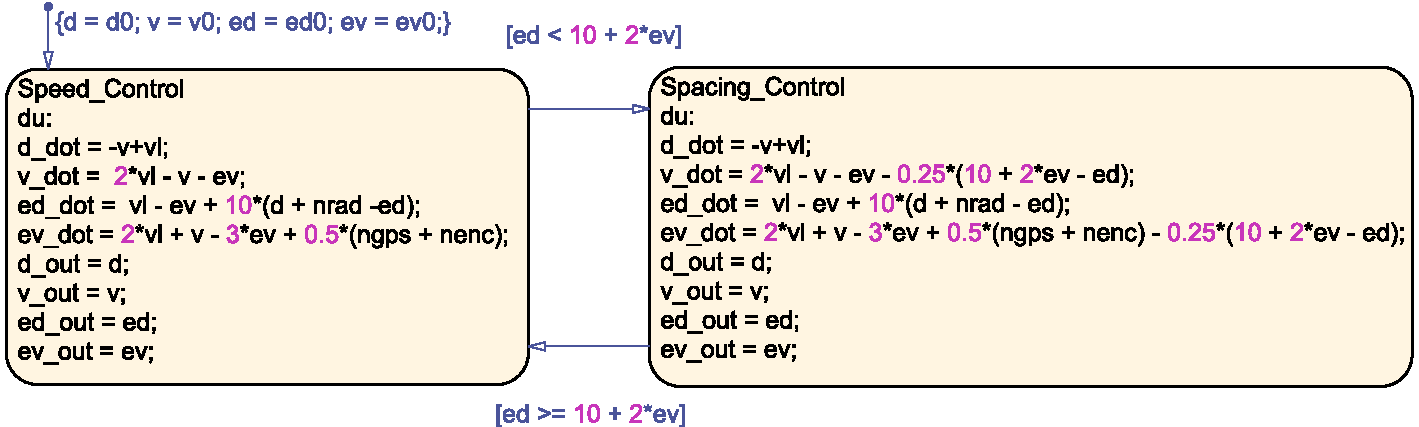
\includegraphics[width=0.48\textwidth]{image/acc_slsf_model}%\vspace{1cm}
		%\includegraphics[trim = 17mm 85mm 17mm 0mm, clip, width=0.95\textwidth]{image/spectral_signal}%
	\caption{The original SLSF model of the ACC system.}%
	\figlabel{acc_slsf_model}%
	\vspace{-1em}
\end{figure}%

\begin{figure}[t!]%
	\centering%
    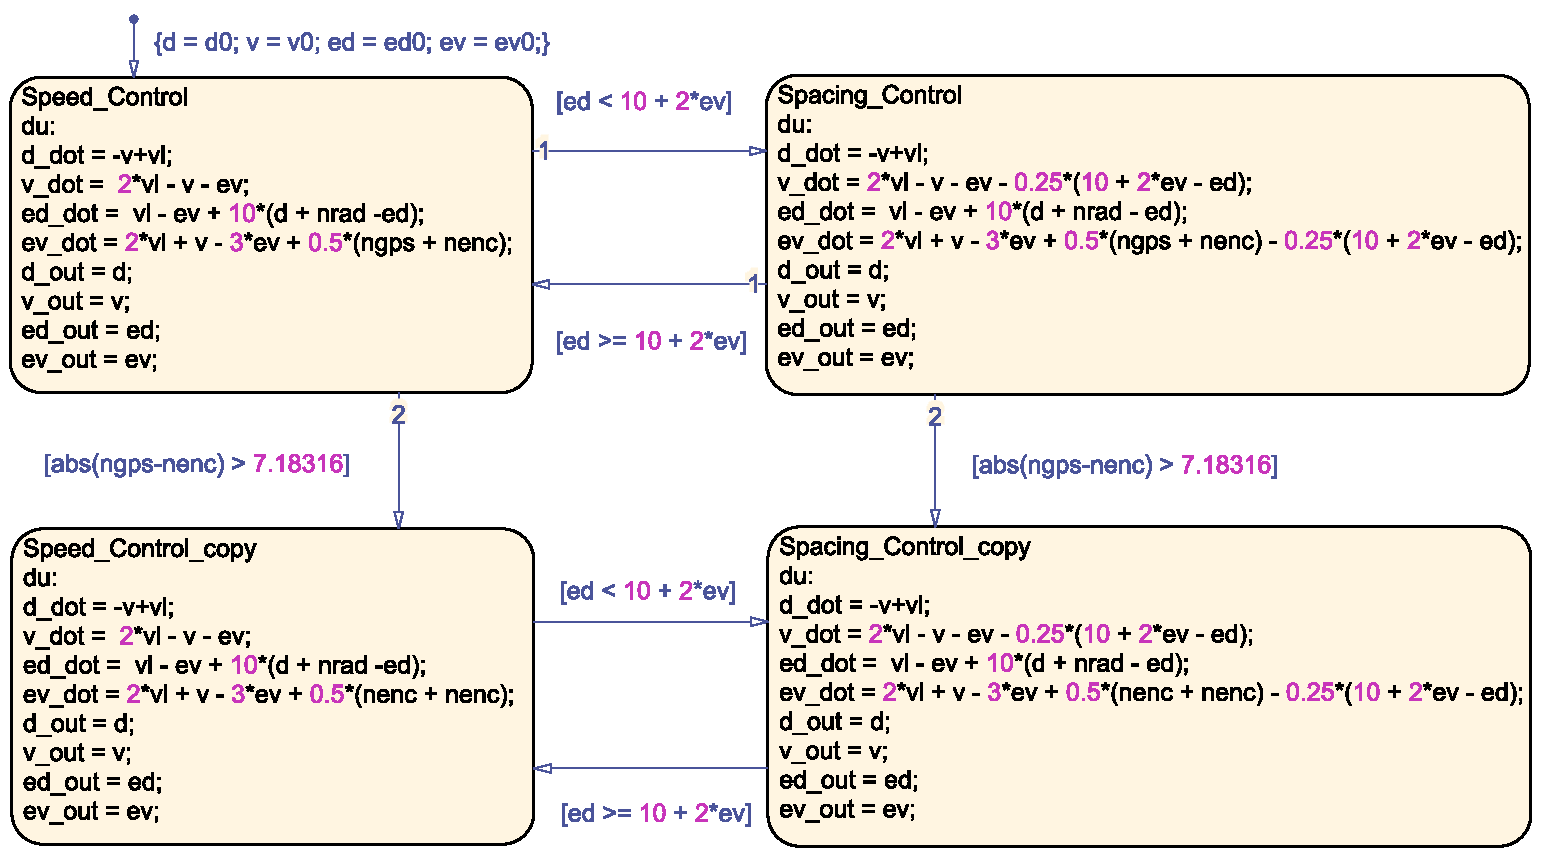
\includegraphics[width=0.48\textwidth]{image/acc_model_pat1}%\vspace{1cm}
		%\includegraphics[trim = 17mm 85mm 17mm 0mm, clip, width=0.95\textwidth]{image/spectral_signal}%
	\caption{The repaired ACC model with a synthesized value of $\theta = 7.08515$.}%
	\figlabel{acc_model_pat1}%
	\vspace{-1em}
\end{figure}%

\vspace{0.5em}
\noindent
{\bf GPS sensor attack.} To perform a spoofing attack on the GPS sensor of the  ACC model, we continuously inject false data to manipulate its measurement value. In this case, we omit the original assumption $|\ngps| \leq 0.05$, and employ the new assumption as $|\ngps| \leq 50$. Using the input generator in Breach, we can specify the GPS spoofing attack as a standard input test signal such as a constant, ramp, step, sinusoid or random signal. The following evaluations of three different resiliency patterns used to repair the ACC model are based on the same assumption that the GPS spoofing occurs at every time point, specified as a random constant signal over the range of [-50, 50] during 50 seconds.
% whose amplitude varies over the range of [-50, 50]

\vspace{0.5em}
\noindent
{\bf Model Repair for the ACC system.} Under the GPS sensor spoofing  attack, the original SLSF model does not satisfy its safety requirement and a designer needs to apply a certain resiliency pattern to repair the model. The \emph{first resiliency pattern} for repairing the ACC system has been introduced in~\secref{overview}, which makes the copy of the original model where the controller ignores the GPS reading as it can no longer be trusted. However, we need to determine the best switching condition from the original model to the copy.~\figref{acc_model_pat1} shows the completed model, where the switching condition is determined by synthesizing the value of $\theta$ over the range of [0, 50] using Breach. For the first pattern, the model transformation takes about 2 seconds, and the synthesis procedure takes approximately 88 seconds over 6 iterations of the falsification loop. %\JW{Fixed: The following figure (figure 6) is unreadable.}



The \emph{second resiliency pattern} for the ACC model is the extended version of the first one where it includes a switching-back condition from the copy to the original model when the GPS sensor attack is detected and mitigated. An example of such a switching-back condition is when the difference between the $\nenc$ and $\ngps$ are getting smaller, \ie $|\ngps -\nenc| < \theta - \epsilon$, where $\epsilon$ is a positive user-defined tolerant. For this pattern, the model transformation script can be written similar to the one shown in~\figref{examplecode} with adding the \emph{addTransition} function from the copy mode to the original mode with the guard condition labeled as $|\ngps -\nenc| < \theta - \epsilon$ in the \emph{formode} loop.
%
The performance of \toolreaffirm for the second pattern is similar to the first pattern with the same synthesized value of $\theta = 7.08515$.

%
\begin{figure}[t!]%frame=none,
\begin{lstlisting}[basicstyle=\ttfamily\footnotesize, numbers=none]

# start a transformation
formode m = model.Mode {
    m.replace(m.flow,"ngps", "2*theta*ngps")
    m.replace(m.flow,"nenc", "2*(1-theta)*nenc")
}
# end of the transformation
\end{lstlisting}
\caption{The third resiliency pattern for the ACC system based on the linear combination of $\nenc$ and $\ngps$.}%
\figlabel{acc_code_3}%
	%\vspace{-0.5em}%

\end{figure}
\begin{figure}[tbp]%
	\centering%
    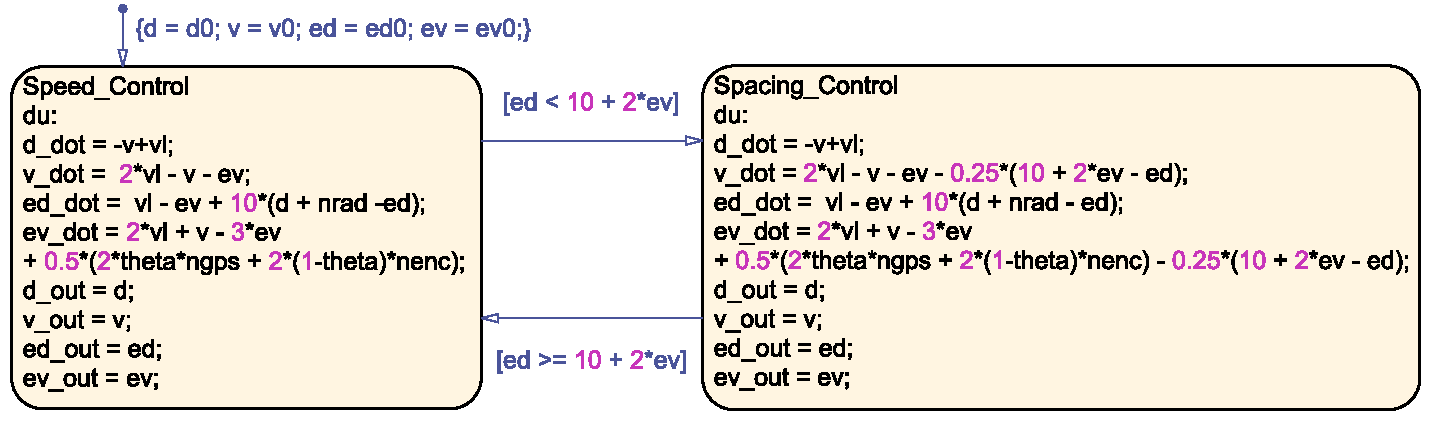
\includegraphics[width=0.48\textwidth]{image/acc_model_pat3}%\vspace{1cm}
		%\includegraphics[trim = 17mm 85mm 17mm 0mm, clip, width=0.95\textwidth]{image/spectral_signal}%
	\caption{The repaired ACC model with a synthesized value of $\theta = 0.1543$ for the resiliency pattern shown in ~\figref{acc_code_3}.}%
	\figlabel{acc_model_pat3}%
	\vspace{-1em}
\end{figure}%


Alternatively, the \emph{third resiliency pattern}, which we do not need to modify the structure of the original model, is to model the redundancy in the sensory information as a linear combination of different sensor measurements. For example, instead of taking the average of $\ngps$ and $\nenc$, we can model their relationship as $\theta\ngps + (1-\theta)\nenc$, and then synthesize the value of $\theta$ so that the safety property is satisfied. The transformation script of this resiliency pattern is given in~\figref{acc_code_3}. For this pattern, we assume that a designer still wants to use all sensor measurements even some of them are under spoofing attacks and would like to search for the value of $\theta$ over the range of [0.2, 0.8] (instead of [0, 1]). Given the same attack model for the other patterns, the synthesizer in \toolreaffirm fails to find the value of $\theta$ within the given range to ensure that the safety property is satisfied. However, if we enlarge the range of $\theta$ to [0.1, 0.9], the synthesizer successfully finds the safe value $\theta = 0.1543$ that appears in the repaired model shown in~\figref{acc_model_pat3}. In this scenario, the model transformation takes about 1.75 seconds, and the synthesis procedure takes approximately 55.78 seconds over 5 iterations of the falsification loop.
%
This result indicates that the third pattern can repair the model if the portion of the GPS measurement contributed to estimating the velocity is significantly smaller than that of the wheel encoders. However, if the GPS spoofing attack specified over a broader range (\eg $|\nenc| \leq 100$), the pattern will fail to repair the model.









\subsection{Single-Machine Infinite-Bus System}
%
\begin{figure}[t!]%
	\centering%
    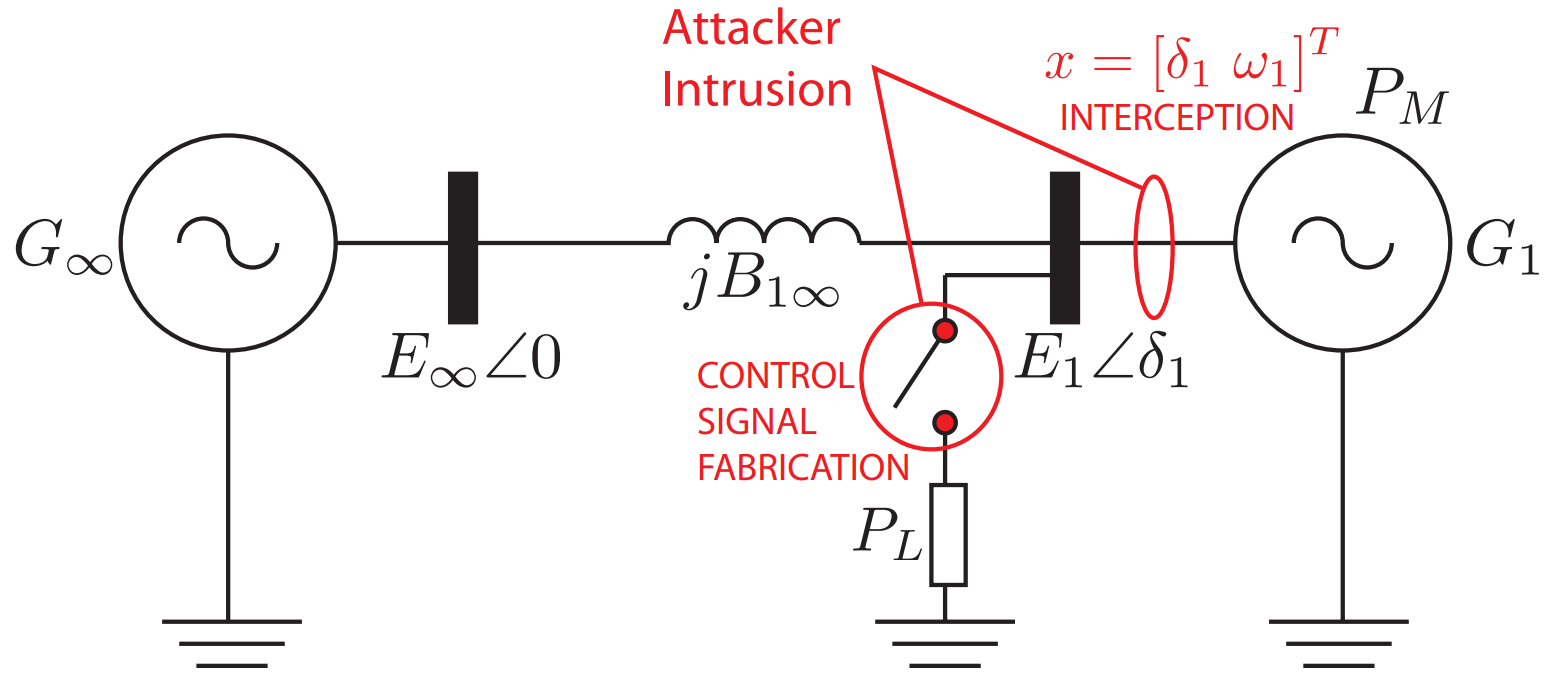
\includegraphics[width=0.42\textwidth]{image/smib}%
		%\includegraphics[trim = 17mm 85mm 17mm 0mm, clip, width=0.95\textwidth]{image/spectral_signal}%
	\caption{Single-machine infinite-bus system~\cite{farraj2014practical}.}%
	\vspace{-1em}
	\figlabel{smib}%
\end{figure}%
Next, we study a class of cyber-physical switching attacks that can destabilize a smart grid system model, and then apply \toolreaffirm to repair the model to provide resilience. A smart power grid system such as the Western Electricity Coordinating Council (WECC) 3-machine, 9-bus system~\cite{sauer1998power}, can be represented as a single-machine infinite-bus (SMIB) system shown\footnote{the figure is copied from \cite{farraj2014practical}.} in~\figref{smib}. In this system, $G_\infty$ and $G_1$ correspondingly represent the SMIB and local generators; $B_\infty$ and $B_1$ denote the infinite and local bus, respectively; $E_\infty$ is the infinite bus voltage; $E_1$ is the internal voltage of $G_1$; $B_{1\infty}$ is the transfer susceptance of the line between $B_1$ and $B_\infty$; and $P_M$ is the mechanical power of $G_1$. The local load $P_L$ is connected or disconnected to the grid by changing a circuit breaker status. The SMIB system is considered as a \emph{switched system} in which the physical dynamics are changed between two operation modes based on the position of the circuit breaker. The system has two states, $\delta_1$ and $\omega_1$, which are the deviation of the rotor angle and speed of $G_1$ respectively, and $x = [\delta_1,\omega_1]^T$ is the state vector of $G_1$.
%
The stability (safety) property of the system can be specified as the following STL formula,
%
\begin{align}
\vspace{-1em}
	\varphi_{SMIB} & = \Box_{[0, T]} (0 \leq \delta_1[t] \leq 3.5) \wedge (-2 \leq \omega_1[t] \leq 3),\formlabel{smib_stl}
		\vspace{-1em}
\end{align}
where $T$ is a simulation duration.

\vspace{0.5em}
\noindent
{\bf Original SLSF Model.} In this paper, we model the SMIB system as the SLSF model displayed in \figref{smib_plant_model}. The model contains two operation modes whose nonlinear dynamics characterize the transient stability of the local generator $G_1$ presented in~\cite{farraj2014practical}. The transitions between two operation modes depend on the status of the circuit breaker which is connected or disconnected to the load.
%
In the model, $\delta_1$ and $\omega_1$ are represented by $delta$ and $omega$, respectively; and the initial conditions are $delta0 \in [0, 1.1198]$ and $omega0 \in [0, 1]$. The discrete variable $load$ captures the open and closed status of the circuit breaker.
%

%
\begin{figure}[tbp]%
	\centering%
    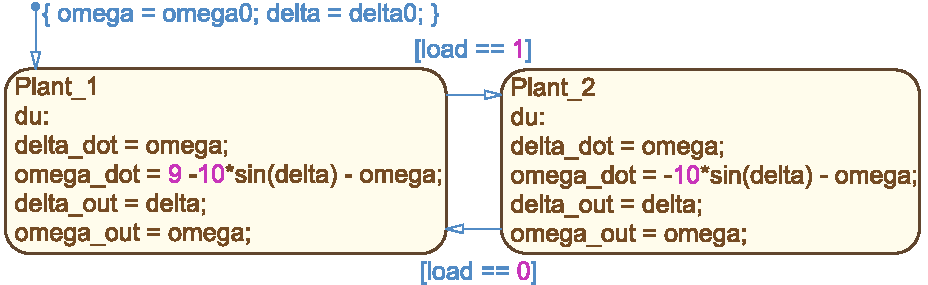
\includegraphics[width=0.48\textwidth]{image/smib_plant_model}%\vspace{1cm}
		\vspace{-1em}
		%\includegraphics[trim = 17mm 85mm 17mm 0mm, clip, width=0.95\textwidth]{image/spectral_signal}%
	\caption{The Stateflow chart models the plant of the SMIB system.}%
	\figlabel{smib_plant_model}%
	\vspace{-1em}
\end{figure}%
%
%
%For an appropriate selection of parameters~\cite{farraj2014practical}, the second-order swing equation which characterizes the transient stability of the local generator $G_1$ can be described as:
%
%\begin{align}
%\dot{\delta_1} & = \omega \nonumber \\
%\dot{\omega} & =
%\begin{cases}
    %-10sin\delta_1 - \omega_1, & \text{if $P_L$ is connected}.\\
    %9 - 10sin\delta_1 - \omega_1, & \text{if $P_L$ is disconnected},
 %\end{cases} \label{eq:smib_dynamics}
%\end{align}
%%
%where, $\delta_1$, $\omega_1$ are the deviation of the rotor angle and speed of $G_1$ respectively, and $x = [\delta_1,\omega_1]^T$ is the state vector of $G_1$.
%%
%%
%
%The swing equation of the SMIB system has an interesting property known as a \emph{sliding mode} behavior. This behavior occurs when the state of the system is attracted and subsequently stays within the \emph{sliding surface} defined by a state-dependent switching signal $s(x)\in\Real$~\cite{decarlo1988variable, liu2014coordinated}. An example of a sliding surface is $s(x) = 0$. When the system is confined on a sliding mode surface, its dynamics exhibit high-frequency oscillations behaviors, so-called a \emph{chattering} phenomenon, which is well-known in the power system design~\cite{sabanovic2004variable}.
%%
%At this moment, if the attacker conducts the fast switches between two operation modes, the system will be steered out of its desirable equilibrium position. As a result, the power system becomes unstable even if each individual subsystem is stand-alone stable~\cite{liu2014coordinated}.
%%



%


\begin{figure}[t!]%
	\centering%
    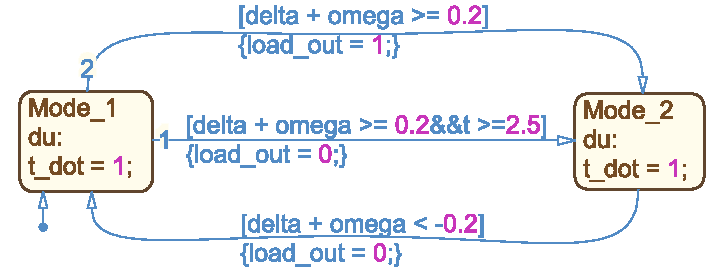
\includegraphics[width=0.42\textwidth]{image/smib_attack_model}%\vspace{1cm}
		\vspace{-1em}
		%\includegraphics[trim = 17mm 85mm 17mm 0mm, clip, width=0.95\textwidth]{image/spectral_signal}%
	\caption{The Stateflow chart models the sliding-mode attack to the SMIB system.}%
	\figlabel{smib_attack_model}%
	\vspace{-1em}
\end{figure}%


\vspace{0.5em}
\noindent
{\bf Sliding-mode attack.} The SMIB system has an interesting property known as a \emph{sliding mode} behavior. This behavior occurs when the state of the system is attracted and subsequently stays within the \emph{sliding surface} defined by a state-dependent switching signal $s(x)\in\Real$~\cite{decarlo1988variable, liu2014coordinated}. An example of a sliding surface is $s(x) = 0$. When the system is confined on a sliding mode surface, its dynamics exhibit high-frequency oscillations behaviors, so-called a \emph{chattering} phenomenon, which is well-known in the power system design~\cite{sabanovic2004variable}. At this moment, if an attacker conducts the fast switches between two operation modes, the system will be steered out of its desirable equilibrium position. As a result, the power system becomes unstable even each individual subsystem is stand-alone stable~\cite{liu2014coordinated}.
%\IL{the system is attacked?}
%To successfully perform a sliding-mode attack to a power grid system, we assume that the attack can a) gain some knowledge about the state information to mathematically construct an unstable sliding surface that can destabilize the system, and b) access to the communication channel to control the circuit breaker position. We note that a sliding-mode attack can be considered as a cyber-physical attack as it requires the attacker to manipulate both physical and cyber parts of the system. For the SMIB model with the swing equation defined as \eqref{smib_dynamics}, an attacker can use a sliding surface $s(x) = \delta_1 + \omega_1$ to calculate the value of the switching signal based on the following equation.
%%
%\begin{align}
%\dot{\delta_1} & = \omega \nonumber \\
%\dot{\omega} & =
%\begin{cases}
    %-10sin\delta_1 - \omega_1, & \text{$s(x) \geq \epsilon$}.\\
    %9 - 10sin\delta_1 - \omega_1, & \text{$s(x) < -\epsilon$},
 %\end{cases}
%\end{align},
%where $\epsilon$ represents switching delays and hysteresis~\cite{liu2011class}.
%
%
%The stages of sliding-mode attack can be summarized as follows. The attacker first switches the circuit breaker to connect the load to the grid. When $\delta_1 + \omega_1 < -\epsilon$, the attacker switches the circuit breaker to disconnect the load; and when $\delta_1 + \omega_1 \geq \epsilon$, the attacker switches the circuit breaker to connect the load. The two switching actions are repeated until the system is driven out of the stability boundary, and then the attacker permanently switches the circuit breaker to disconnect the load.
%

%\vspace{0.5em}
%\noindent
%{\bf Original SLSF model of the SMIB system.}
%In this paper, we model the sliding-mode attack to the SMIB system as an SLSF diagram including two Stateflow models, where the plant model displayed in \figref{smib_plant_model} represents the physical dynamics of the system and the attack model is shown in \figref{smib_attack_model}.
%
%In the plant model, $\delta_1$ and $\omega_1$ are represented by $delta$ and $omega$, respectively; and the initial conditions are $delta0 \in [0, 1.1198]$ and $omega0 \in [0, 1]$. The discrete variable $load$ captures the open and closed status of the circuit breaker.
%
To perform the sliding-mode attack on the original SMIB model, we model the attack as the SLSF model shown in \figref{smib_attack_model}. In this model, we assume that the attacker selects a sliding surface $s(x) = \delta_1 + \omega_1 = 0.2$, and the local variable $t$ captures a simulation duration. We note that two transitions from the first mode to the second mode are executed with priorities such that the load is permanently disconnected at some instance where $t \geq 2.5$ seconds. More details of the stages to construct the sliding-mode attack can be found in~\cite{farraj2014practical}.
%
%
\figref{smib_result} illustrates the examples of stable (\ie without an attack) and unstable (\ie a counterexample appearing under the sliding-model attack) behaviors of the SMIB system returned by running the falsifier of Breach, respectively. The red box defines the stable (safe) operation region of the SMIB system that can be formalized by the STL formula $\varphi_{SMIB}$.
%
\begin{figure}[!t]%frame=none,
\begin{lstlisting}[basicstyle=\ttfamily\footnotesize, numbers=none]
# start a transformation
model.addParam("theta") # add a new parameter theta
model.addLocalVar("clock") # add a clock variable
formode m = model.Mode {
    m.addFlow("clock_dot = 1")
}
fortran t = model.Trans {
		# a transition only triggers after theta seconds
    t.addGuardLabel("&&","clock > theta")
		# reset a clock after each transition
    t.addResetLabel("clock = 0")
}
# end of the transformation
\end{lstlisting}
	\vspace{-0.5em}
\caption{A dwell-time resiliency pattern for the SMIB system.}%
\vspace{-1em}
\figlabel{smib_code}%
	%\vspace{-0.5em}%
\end{figure}

\begin{figure}[tbp]%
	\centering%
    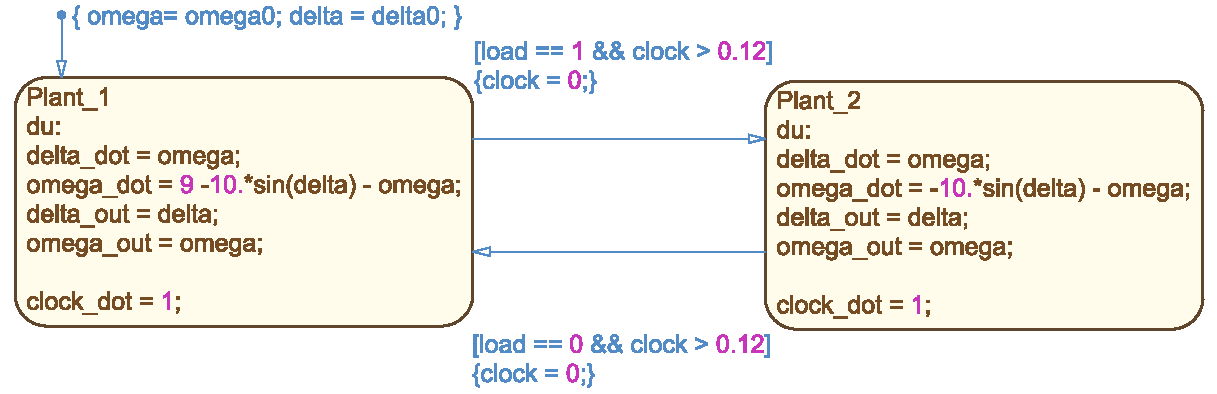
\includegraphics[width=0.48\textwidth]{image/smib_plant_model_res}%\vspace{1cm}
			\vspace{-0.5em}
		%\includegraphics[trim = 17mm 85mm 17mm 0mm, clip, width=0.95\textwidth]{image/spectral_signal}%
	\caption{The repaired SMIB model with a synthesized dwell-time.}%
	\figlabel{smib_plant_model_res}%
\vspace{-1em}
\end{figure}%



\begin{figure*}[t!]%
	\centering%
    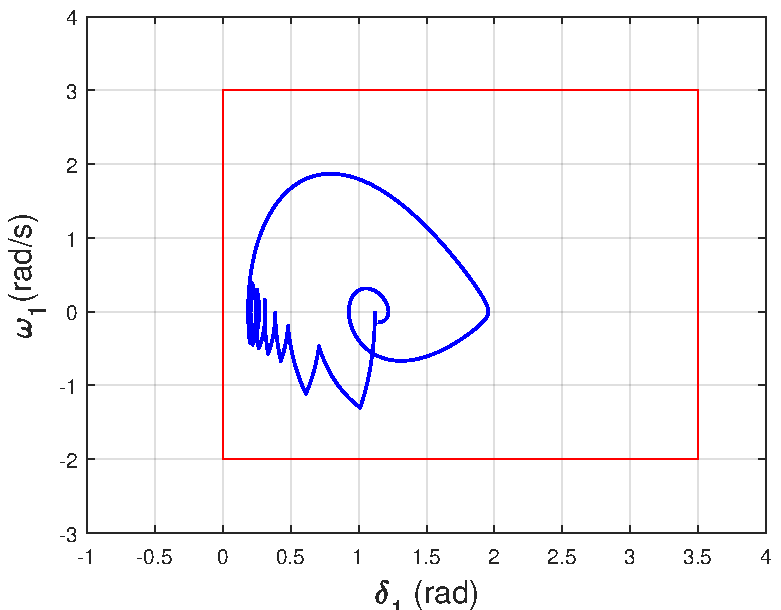
\includegraphics[width=0.31\textwidth]{image/normal}%\vspace{1cm}
		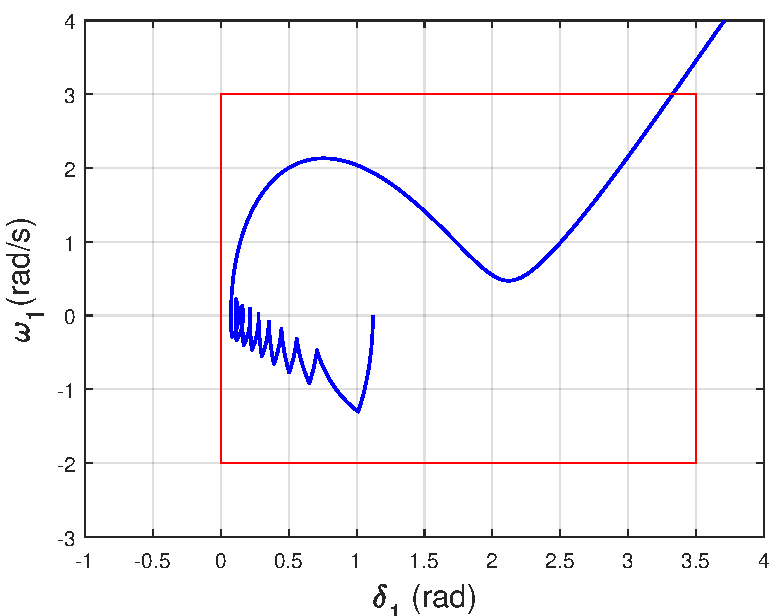
\includegraphics[width=0.307\textwidth]{image/counter}%
		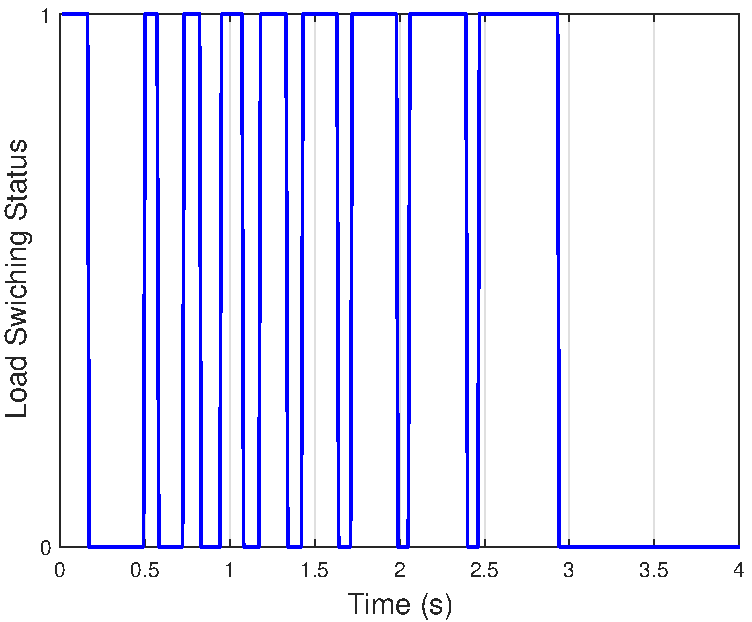
\includegraphics[width=0.294\textwidth]{image/load_v2}%
		%\vspace{-0.5em}
		%\includegraphics[trim = 17mm 85mm 17mm 0mm, clip, width=0.95\textwidth]{image/spectral_signal}%
	\caption{From left to right: 1) the stable system trajectory without an attack, 2) the counterexample represents the unstable system trajectory under the sliding-mode attack, and 3) the status of a circuit breaker during the attack, where 0 and 1 represent the disconnection and connection of the load $P_L$, respectively.}%
	\figlabel{smib_result}%
	%\vspace{-0.5em}
\end{figure*}%




\vspace{0.5em}
\noindent
{\bf Model Repair for the SMIB system.}
As a sliding-mode attack is constructed based on switching back-and-forth the circuit breaker quickly to trap the system inside the sliding surface before guiding its state variables evolving outside the stability boundary, a potential strategy to mitigate such an attack is to increase the minimum switching time of the circuit breakers. Indeed, the designer can repair the original model by including a minimum dwell time in each mode of the system to prevent rapid switching.~\figref{smib_code} shows a resiliency pattern written as a HATL script that introduces the \emph{clock} variable as a timer, and the switching time relies on the value of $\theta$.

The model transformation of \toolreaffirm takes the dwell-time pattern shown in~\figref{smib_code}, and then convert the model to a new version that integrates the pattern with the unknown parameter $\theta$.
%
Then, the model synthesis of \toolreaffirm calls Breach to search for the best (\ie minimum) value of $\theta$ over and the range of $[0, 0.3]$ that ensures the final model satisfies $\varphi_{SMIB}$ (with $T = 10$ seconds) under the sliding-mode attack. The final model, which is stable, and its simulation trajectories contain within a red box similar to the most left subfigure shown in \figref{smib_result}, is displayed in~\figref{smib_plant_model_res}, where the synthesized value of $\theta$ equals to $0.12$. Overall, the model transformation takes about 2 seconds, and the synthesis procedure takes approximately 45 seconds over 8 iterations of the falsification loop.



%\vspace{0.5em}
%\noindent
%{\bf Repaired SMIB Model.} Given a resiliency pattern shown in ~\figref{smib_code},

%!TEX root = main.tex
\section{Related Works}
\seclabel{rw}
%
%The idea of our methodologies proposed in this paper is inspired from the concept of \emph{program sketching}~\cite{solar2013program,solar2005programming}, and the recent works on completion of distributed protocols~\cite{alur2017automatic, alur2015automatic, alur2014synthesizing}. Given a model of the \emph{incomplete} distributed protocol, which is a set of communicating finite-state processes with incomplete transition relations, a model of the environment, and its correctness requirements specified in temporal logic~\cite{clarke2000model}, determine a \emph{completion} of the finite state machines (FSMs) for the processes such that the composition satisfies all the requirements. This approach can be viewed as a fruitful collaboration between the designer and the synthesis tool where a programmer needs to provide a \emph{skeleton} of the desired protocol, and some details that the programmer is unsure about, for instance, regarding corner cases and handling of unexpected messages, and the synthesizer will automatically complete it with adding transitions.
%%
%%
%Instead of synthesizing a \emph{complete} FSM, we address the problem of automatic repair of CPSs modeled as hybrid automata.%, which is an extended FSM with a set of real-valued variables evolving continuously over intervals of real-time.  
%
%
%
%In our approach, a designer needs to provide a model transformation script that transforms an initial model to a new version whose parameters values will be determined by the synthesizer to provide resilience. 
%

\vspace{0.5em}
\noindent
{\bf Model-based design of resilient CPSs.} Examples of model-based approaches to ensure resiliency include the approach proposed in~\cite{fitzgerald2012rigorous} that can be used to design a resilient CPS through co-simulation of discrete-event models, a modeling and simulation integration platform for secure and resilient CPS based on attacker-defender games proposed in~\cite{koutsoukos2018sure} with the corresponding testbed introduced in~\cite{neema2018integrated}, the resilience profiling of CPSs presented in~\cite{jackson28resilience}, and the recent works of the design, implementation, and monitor of attack-resilient CPSs introduced in \cite{weimer2018parameter,pajic2017design}.   
%
Although these approaches can leverage the modeling and testing for a resilient CPS, they do not offer a model repair mechanism as well as a generic approach to design a resiliency pattern when vulnerabilities are discovered. Our proposed method is complementary to those works as we provide a generic, programmable way for a designer to specify a potential edit that can effectively repair the model for improving resiliency.

\vspace{0.5em}
\noindent
{\bf Formal analysis of hybrid systems.} Our approach utilizes Breach to synthesize an SLSF model due to its advantages in performing  falsification, systematic testing and parameter synthesis for hybrid systems. However, Breach cannot give a formal proof of the system correctness. Depending on different types of hybrid systems, other automatic verification tools can be considered to perform a reachability analysis or formally prove whether a system satisfy a given safety property. For examples, d/dt~\cite{asarin2002d} and SpaceEx~\cite{frehse2011cav} and  are well-known verification tool for linear/affine hybrid systems; Flow*\cite{chen2013flow} and dReach\cite{kong2015dreach} can be used to compute a reachable set of nonlinear hybrid automata; and C2E2 is a verification tool for Stateflow models~\cite{duggirala2015c2e2}. 
%
However, scalability is the main factor that limits the applications of those verification approaches to the formal analysis of hybrid systems. 

  
\vspace{0.5em}
\noindent
{\bf Model transformation languages of hybrid systems.} In the context of the model transformation, GREAT is a metamodel-based graph transformation language that can be used to perform different transformations on domain-specific models~\cite{agrawal2003graph, agrawal2003end}. GREAT has been used to translate SLSF models to Hybrid Systems Interchange Format (HSIF)~\cite{agrawal2004semantic}. Such a translation scheme is accomplished by executing a sequence of translation rules described using UML Class Diagram in a specific order. %
% 
Other approaches that also perform a translation from Simulink diagrams to hybrid systems formalisms such as Timed Interval Calculus~\cite{chen2009formal}, Hybrid Communicating Sequential Processes~\cite{liu2010calculus}, Lustre~\cite{tripakis2005translating}, and SpaceEx~\cite{minopoli2016sl2sx}.  
%
HYST~\cite{bak2015hyst} is a conversion tool for hybrid automata which allows the same model to be analyzed simultaneously in several hybrid systems analysis tools. HYST takes a source input model in SpaceEx XML format~\cite{frehse2011spaceex}, parses it to an intermediate representation, and then prints a resulting output to some desired formats. HYST can automatically translate hybrid automata to \emph{trajectory-equivalent} SLSF models, which enables a \emph{correct-by-construction} compositional design for CPS with embedding hybrid automata into large-scale SLSF models~\cite{bak2017hybrid}.  
%
Unlike these approaches that focus on the translations between different hybrid system modeling frameworks, our goal is to provide a lightweight programmable model transformation language for hybrid systems in which a designer only needs to write a simple script to repair a CPS model.  
 
%




%Given an \emph{incomplete} hybrid automata contains missing variables, transition relations and operation modes, a \emph{transformation script} that repair the \emph{incomplete} model to the model with unknown parameters, and a set of correctness requirements specified in STL, search

%Our proposed model synthesis tool of \toolreaffirm keeps the given architectural model unchanged, but modifies the behavioral model to make sure the new model always satisfies a set of requirements. The overall strategy is inspired by the protocol completion tool mentioned above.


%in which the programmer need to specify an \emph{incomplete} protocol to be completed by the synthesizer so as to satisfy all the correctness requirements. This methodology for protocol specification can be viewed as a fruitful collaboration between the designer and the synthesis tool: the programmer has to describe the structure of the desired protocol, but some details that the programmer is unsure about, for instance, regarding corner cases and handling of unexpected messages, are filled in automatically by the tool.


%An alternative and potentially more feasible approach inspired by \emph{program sketching} \cite{solar2013program,solar2005programming}, is to ask the programmer to specify an \emph{incomplete} protocol to be completed by the synthesizer so as to satisfy all the correctness requirements. This methodology for protocol specification can be viewed as a fruitful collaboration between the designer and the synthesis tool: the programmer has to describe the structure of the desired protocol, but some details that the programmer is unsure about, for instance, regarding corner cases and handling of unexpected messages, are filled in automatically by the tool.


%
%Given an \emph{incomplete} hybrid automata contains missing variables, transition relations and operation modes, a transformation script that specifies the potential \emph{transformation}  of the \emph{incomplete} model to the model with unknown parameters, and a set of correctness requirements specified in STL, search
%
%
%A distributed protocol traditionally is modeled as a set of communicating finite-state processes, and both safety and liveness requirements specify its correctness. 


%given a set of finite state machines (FSMs) for communicating processes with incomplete transition functions, a model of the environment, and a set of safety and liveness requirements, find a completion of the Finite State Machines for the processes such that the composition satisfies all the requirements. 

%Next, we will describe some recent works on completion of distributed protocols that will be the basis of our approach proposed in this paper~\cite{alur2017automatic, alur2015automatic, alur2014synthesizing}. A
%
%A distributed protocol traditionally is modeled as a set of communicating finite-state processes, and both safety and liveness requirements specify its correctness. 
%
%In \emph{model checking}, a given a model of the distributed protocol is checked against its correctness requirements specified in temporal logic~\cite{clarke2000model}. In \emph{reactive synthesis}, the goal is to automatically derive a protocol from the given logical requirements, but this turns out to be computationally intractable~\cite{finkbeiner2016synthesis}. An alternative and potentially more feasible approach inspired by \emph{program sketching} \cite{solar2013program,solar2005programming}, is to ask the programmer to specify an \emph{incomplete} protocol to be completed by the synthesizer so as to satisfy all the correctness requirements. This methodology for protocol specification can be viewed as a fruitful collaboration between the designer and the synthesis tool: the programmer has to describe the structure of the desired protocol, but some details that the programmer is unsure about, for instance, regarding corner cases and handling of unexpected messages, are filled in automatically by the tool.

%The \emph{protocol synthesis problem} then reduces to the following \emph{protocol completion problem}: given a set of finite state machines (FSMs) for communicating processes with incomplete transition functions, a model of the environment, and a set of safety and liveness requirements, find a completion of the Finite State Machines for the processes such that the composition satisfies all the requirements. The computational complexity of this problem is the same as that of model checking of distributed protocols. However, now we need to cope with a search with two nested exponentials: the number of possible completions of the incomplete input model is exponential and so is the number of states of the product of all the component processes for any given completion. Advances in model checking offer a way of dealing with the latter, while \emph{counterexample-guided inductive synthesis} (CEGIS) is a new technology that is a potential solution for the former~\cite{alur2013syntax,seshia2015combining,solar2005programming}.
%\vspace{-0.5em}
\section{Conclusion and Future Work}
%\section{Conclusion}
\seclabel{conclude}
%
In this paper, we have presented a new methodology and the tool-chain \toolreaffirm that effectively assist a designer to repair CPS models under unanticipated attacks automatically. 
%
The model transformation tool takes a resilient pattern specified in the transformation language HATL and generates a new model including unknown parameters whose values can be determined by the synthesizer tool such that the safety requirement is satisfied.
%
We demonstrated the high-applicability of \toolreaffirm by using the tool-chain to efficiently repair CPS models under realistic attacks including the ACC models under the GPS sensor spoofing attack and the SMIB models under the sliding-model attack.

\vspace{0.5em}
\noindent
{\bf Future Work}

%
%\vspace{0.25em}
%\paragraph*{Future Work} %There are several directions for the future work of HyperSTL. 
%We first plan to introduce a library of HyperSTL fomulae that encapsulates different general classes of hyperproperties of CPS including those presented in this paper.
%%
%Second, the falsification algorithm of HyperSTL proposed in the paper is incomplete as it relies on self-composition (i.e. making copies of a system) and only falsifies a restricted class of hyperproperties. 
%%
%Thus, extending the falsification algorithm to bypass self-composition to falsify more interesting hyperproperties is planned. Also, the monitoring algorithms of HyperLTL recently proposed in~\cite{brett2017rewriting, agrawal2016runtime} could be applied to HyperSTL.
%%
%%On the other hand, we will also leverage the testing framework of HyperSTL to falsify a hyperproperty with finite-simulation guarantees.% and evaluate the performance of a bug-finding technique using industrial Simulink models.
%
%
%%In future work, we will improve a monitoring algorithm for HyperSTL and apply it to find falsifying traces for hyperproperties of industrial Simulink models.

%\vspace{-1em}
%\input{conclusion}
%\vspace{-1em}
%\renewcommand{\baselinestretch}{0.6}
%\scriptsize
%
\bibliographystyle{ACM-Reference-Format}
%\bibliography{sigproc} 
% \bibliographystyle{abbrv}
\bibliography{luan}  % sigproc.bib is the name of the Bibliography in this case
\end{document}
